\part{常见的心脏病、电解质紊乱及抗心律失常药物所致的心电图改变}

本篇根据先天性心脏病、后天性心脏病、各类心肌病、电解质紊乱、药物影响顺序进行编写。主要讲述先天性、后天性心脏病的病理生理改变与心电图表现的相关性及其特征,以及电解质紊乱、药物对心脏的影响所产生的心电图改变,并将心脏血管支配部位、心脏电生理特性等基础知识有机地融进各个章节之中,共6章。

\protect\hypertarget{text00049.html}{}{}

\protect\hypertarget{text00049.htmlux5cux23chapter49}{}{}

\chapter{常见的先天性心脏病的心电图改变}

\protect\hypertarget{text00049.htmlux5cux23subid580}{}{}

\section{法洛四联症}

1.病理生理改变

法洛四联症包括肺动脉狭窄、室间隔缺损、主动脉骑跨及右心室肥大。其血流动力学改变主要是由肺动脉狭窄引起右心室收缩期负荷过重,导致右心室肥厚(主要表现为右心室肥厚、肺动脉圆锥显著膨隆、室上嵴增厚及右心室内乳头肌和肉柱显著增粗)和右心房肥大,晚期可伴有右心室腔扩张。肥厚的右心室可将左心室推向左后方,右心暴露面增多,占据心尖部。通常以肺动脉瓣下2cm处右心室前壁肌层厚度>0.5cm(正常约0.3~0.4cm)作为右心室肥厚的诊断标准。

2.心电图特征

(1)先心型P波:Ⅱ、Ⅲ、aVF、V\textsubscript{1} 、V\textsubscript{2}
等导联P波高尖,肢体导联电压≥0.25mV,V\textsubscript{1}
、V\textsubscript{2} 导联电压≥0.15mV,V\textsubscript{5}
导联电压≥0.2mV,P波时间大多正常。

(2)电轴右偏:常>+110°。

(3)aVR导联QRS波群呈qR或QR型,q(Q)/R<1,R波电压>0.5mV。

(4)V\textsubscript{1}
导联QRS波形依据肥厚程度可呈qR型、R型、Rs型,R/s>1及rsR′型,R波电压显著增高等。

(5)V\textsubscript{5} 、V\textsubscript{6}
导联QRS波群可呈RS型,R/S<1或rS型等。

(6)V\textsubscript{1} 、V\textsubscript{2}
导联可伴有ST段压低、T波倒置(图\ref{fig41-1})。

\begin{figure}[!htbp]
 \centering
 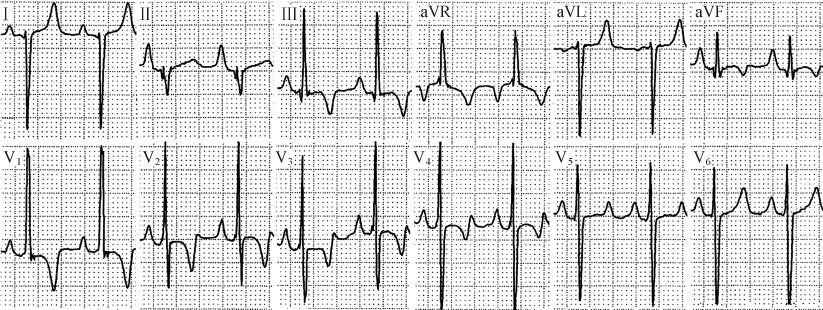
\includegraphics[width=5.5625in,height=2.09375in]{./images/Image00683.jpg}
 \captionsetup{justification=centering}
 \caption{女性,16岁,法洛四联症患者,出现右心房及右心室肥大、下壁异常Q波}
 \label{fig41-1}
  \end{figure} 

\protect\hypertarget{text00049.htmlux5cux23subid581}{}{}

\section{房间隔缺损}

房间隔缺损为最常见的先天性心脏病,包括继发孔缺损型、原发孔缺损型及高位缺损型等。

1.病理生理改变

由于右心室同时接受上、下腔静脉和左心房流入右心房的血液,导致右心室舒张期负荷过重,出现右心房、右心室肥大及扩张。原发孔缺损型房间隔缺损,大多形成部分或完全性房室通道,左束支明显向后下移位,导致左前分支相对发育不良,易出现一度房室传导阻滞及电轴左偏;若伴有二尖瓣关闭不全,则可出现左心室肥大。

2.继发孔缺损型的心电图特征(图\ref{fig41-2})

\begin{figure}[!htbp]
 \centering
 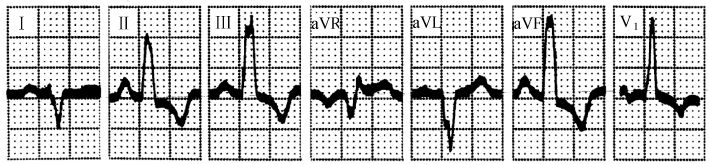
\includegraphics[width=4.79167in,height=1.10417in]{./images/Image00684.jpg}
 \captionsetup{justification=centering}
 \caption{女性,44岁,先心病、继发孔型房间隔缺损。心电图显示右心房肥大、完全性右束支阻滞、提示合并右心室肥大、钩型R波(引自陈琪)}
 \label{fig41-2}
  \end{figure} 

(1)右心房肥大:Ⅱ、Ⅲ、aVF导联P波高尖,电压≥0.25mV;V\textsubscript{1}
、V\textsubscript{2} 导联正相波高尖,电压≥0.15mV。

(2)电轴右偏:一般为轻、中度右偏。右偏越严重,表明右心室肥大越明显。

(3)不完全性或完全性右束支阻滞图形:V\textsubscript{1}
导联QRS波群呈rsR′型或rsr′型,时间多<0.12s,与右心室流出道、室上嵴及圆锥部肥厚有关,有一定的诊断意义。

(4)右心室肥大。

(5)出现钩形R波:Ⅱ、Ⅲ、aVF导联QRS波群起始后80ms内,即R波升肢或顶峰部位出现切迹呈钩形。

(6)可出现一度房室传导阻滞及各种的房性心律失常。

3.原发孔缺损型的心电图特征(图\ref{fig41-3})

\begin{figure}[!htbp]
 \centering
 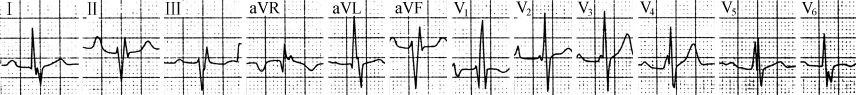
\includegraphics[width=5.78125in,height=0.63542in]{./images/Image00685.jpg}
 \captionsetup{justification=centering}
 \caption{男性,17岁,先心病、原发孔型房间隔缺损伴二尖瓣瓣裂。心电图显示右心房及右心室肥大、电轴-30°、V\textsubscript{1}Ptf值明显增大(提示左心房负荷过重)、一度房室传导阻滞(P-R间期0.24s)、提示不完全性右束支阻滞、侧壁轻度T波改变(Ⅲ、V\textsubscript{3}~V\textsubscript{5} 导联定准电压均为0.5mV)}
 \label{fig41-3}
  \end{figure} 


(1)右心房肥大。

(2)电轴左偏:约-30°,类似左前分支阻滞图形,而有别于继发孔缺损型的心电图改变。

(3)一度房室传导阻滞:P-R间期延长(≥0.24s)。

(4)不完全性或完全性右束支阻滞图形。

(5)右心室肥大或合并左心室肥大。

(6)房性心律失常。

\protect\hypertarget{text00049.htmlux5cux23subid582}{}{}

\section{室间隔缺损}

1.病理生理改变

室间隔缺损包括膜部缺损和肌部缺损两种。当缺损较小,左向右分流量少时,血流动力学变化不明显,心电图可正常;当缺损较大,左向右分流量较大时,导致左、右心室舒张期负荷过重,出现左、右心室肥大或以左心室肥大为主;当左向右分流量很大时,出现轻、中度肺动脉高压,产生双心室肥大;出现重度肺动脉高压时,右心室收缩期负荷过重,导致右心室显著肥大和右心房负荷过重及肥大,此时分流量反而减少,甚至出现逆向分流。

2.心电图特征(图\ref{fig41-4})

\begin{figure}[!htbp]
 \centering
 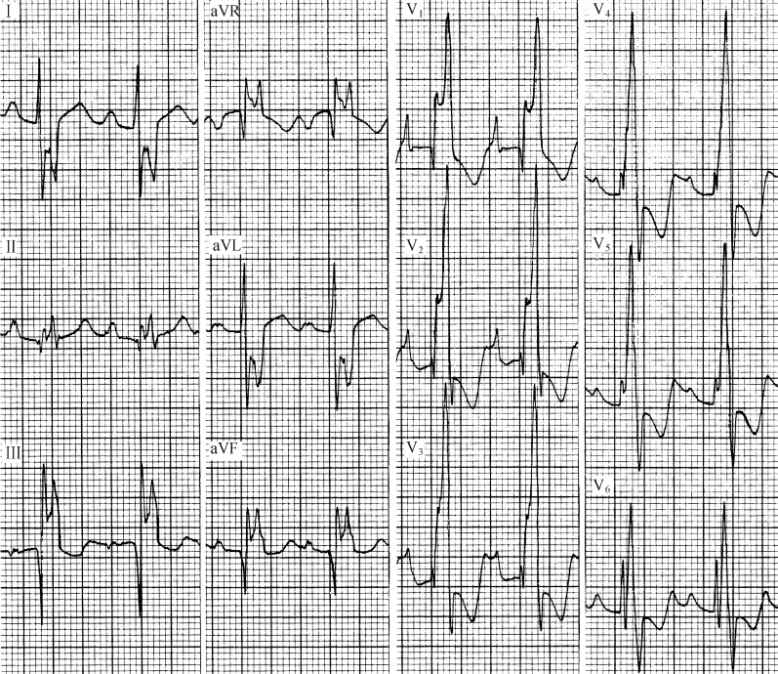
\includegraphics[width=5.38542in,height=4.65625in]{./images/Image00686.jpg}
 \captionsetup{justification=centering}
 \caption{男性,28岁,先心病、室间隔缺损。显示右心房肥大、双心室肥大、下壁异常Q波、完全性右束支阻滞、ST-T改变}
 \label{fig41-4}
  \end{figure} 

(1)心电图正常。

(2)单纯左心室肥大:呈左心室舒张期负荷过重图形,表现为V\textsubscript{5}
、V\textsubscript{6} 导联R波电压增高,ST段轻度抬高,T波高耸。

(3)双心室肥大。

(4)右心室肥大。

(5)P波高大。

(6)可出现各种心律失常

\protect\hypertarget{text00049.htmlux5cux23subid583}{}{}

\section{动脉导管未闭}

1.病理生理改变

未闭的动脉导管位于主动脉峡部和左肺动脉根部,血流从主动脉分流入肺动脉,使肺循环血流量增多,回流至左心房和左心室血流增加,导致左心室舒张期负荷过重,出现左心房、左心室肥大;当发生肺动脉压力增高时,分流量反而减少,出现右心室肥大。

2.心电图特征

(1)心电图正常:见于细小的动脉导管未闭,分流量不大,肺动脉压力不高。

(2)左心房、左心室肥大:P波增宽呈双峰切迹,V\textsubscript{1}
Ptf负值增大;QRS波群呈左心室舒张期负荷过重图形。见于中等大小的动脉导管未闭,肺动脉压力轻、中度增高者(>60mmHg)。

(3)双心房、双心室肥大:见于粗大的动脉导管未闭,肺动脉压力重度增高者(>90mmHg)。

(4)右心室肥大掩盖左心室肥大:当肺动脉压力长期重度增高时,右心室肥大更为明显,可掩盖左心室肥大的心电图改变。

\protect\hypertarget{text00049.htmlux5cux23subid584}{}{}

\section{三尖瓣下移畸形}

1.病理生理改变

三尖瓣下移畸形又称为Ebstein畸形,指部分或整个有效的三尖瓣环向下移位,使右心房增大,右心室缩小,出现右心室一部分心房化,存在三尖瓣返流,常伴有房间隔缺损。

2.心电图特征

(1)右心房扩大:Ⅱ、Ⅲ、aVF导联和V\textsubscript{1} 、V\textsubscript{2}
导联P波高尖,有学者称之为喜马拉雅P波(图\ref{fig41-5})。

\begin{figure}[!htbp]
 \centering
 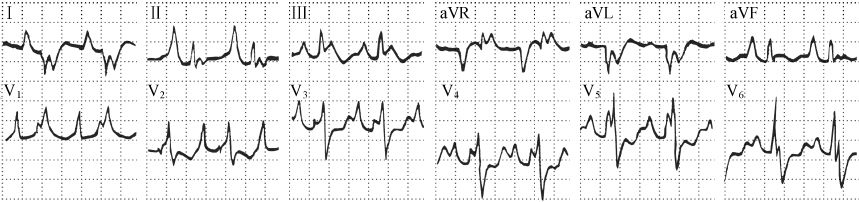
\includegraphics[width=5.80208in,height=1.36458in]{./images/Image00687.jpg}
 \captionsetup{justification=centering}
 \caption{Ebstein畸形患者,出现右心房扩大、一度房室传导阻滞(P-R间期0.24s)、完全性右束支阻滞、前侧壁ST段改变、下壁T波改变(引自临床心电学杂志)}
 \label{fig41-5}
  \end{figure} 

(2)右束支阻滞和V\textsubscript{1} 、V\textsubscript{2}
导联r(R)波和s波低小,为本病特征性的心电图改变。

(3)约25\%患者存在B型预激综合征,出现B型预激与右束支阻滞图形并存的现象(图\ref{fig41-6})。

(4)常出现房室折返性心动过速等心律失常

\begin{figure}[!htbp]
 \centering
 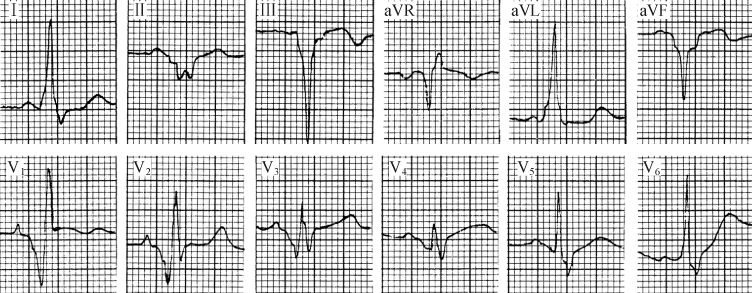
\includegraphics[width=5.08333in,height=1.97917in]{./images/Image00688.jpg}
 \captionsetup{justification=centering}
 \caption{女性,51岁,Ebstein畸形。出现V\textsubscript{1}、V\textsubscript{2} 导联P波略高尖、B型预激综合征合并完全性右束支阻滞}
 \label{fig41-6}
  \end{figure} 


\protect\hypertarget{text00049.htmlux5cux23subid585}{}{}

\section{右位心}

广义的右位心包括镜像右位心、右旋心和心脏右移(图\ref{fig41-7})。通常所说的右位心仅指镜像右位心。

\begin{figure}[!htbp]
 \centering
 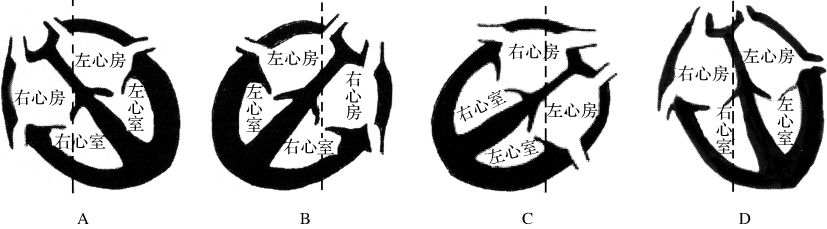
\includegraphics[width=5.58333in,height=1.54167in]{./images/Image00689.jpg}
 \captionsetup{justification=centering}
 \caption{心脏右位的解剖示意图(图A正常、图B镜像右位心、图C右旋心、图D心脏右移)}
 \label{fig41-7}
  \end{figure} 

1.镜像右位心

心脏位于右侧胸腔内,左右心房、心室的关系发生反位,宛如正常心脏的镜中像,可伴有其他内脏的转位。心电图检查对镜像右位心的诊断具有确诊价值,但需排除左、右手的导联线反接。心电图具有以下5个特征:

(1)Ⅰ导联P、QRS、T波均倒置,为正常Ⅰ导联图形的倒镜像改变。

(2)Ⅱ导联和Ⅲ导联、aVR导联与aVL导联的图形互换,而aVF导联图形不变。

(3)胸前导联V\textsubscript{1} ~V\textsubscript{6}
的R波振幅逐渐减低,而S波逐渐加深。

(4)加做右胸导联V\textsubscript{3} R、V\textsubscript{4}
R、V\textsubscript{5} R、V\textsubscript{6}
R,其R波振幅逐渐增高或者以V\textsubscript{4} R、V\textsubscript{5}
R导联R波振幅最高。

(5)将左、右手的导联线反接,用V\textsubscript{2} 、V\textsubscript{1}
、V\textsubscript{3} R、V\textsubscript{4} R、V\textsubscript{5}
R、V\textsubscript{6} R导联分别代表V\textsubscript{1}
、V\textsubscript{2} 、V\textsubscript{3} 、V\textsubscript{4}
、V\textsubscript{5} 、V\textsubscript{6}
导联,即可得到一幅和正常人完全相同的心电图波形(图\ref{fig41-8}、图\ref{fig41-9})。

\begin{figure}[!htbp]
 \centering
 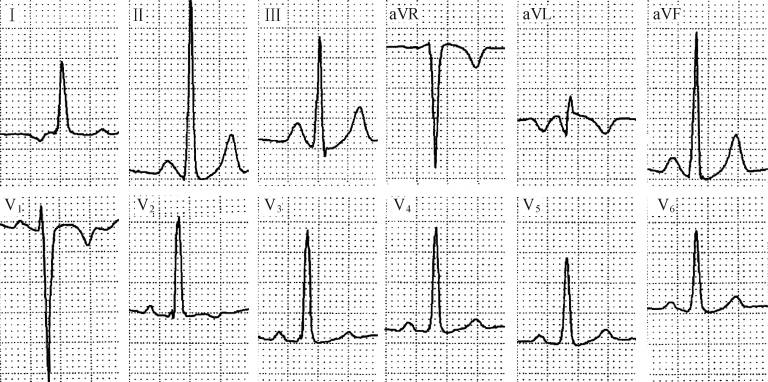
\includegraphics[width=5.1875in,height=2.58333in]{./images/Image00690.jpg}
 \captionsetup{justification=centering}
 \caption{女性,36岁,右位心、风心病、二尖瓣狭窄伴关闭不全。肢体导联心电图显示右位心特点,而胸前导联则显示正常情况下QRS-T波群特点,除此以外,尚显示P波高大、左心室高电压}
 \label{fig41-8}
  \end{figure} 

\begin{figure}[!htbp]
 \centering
 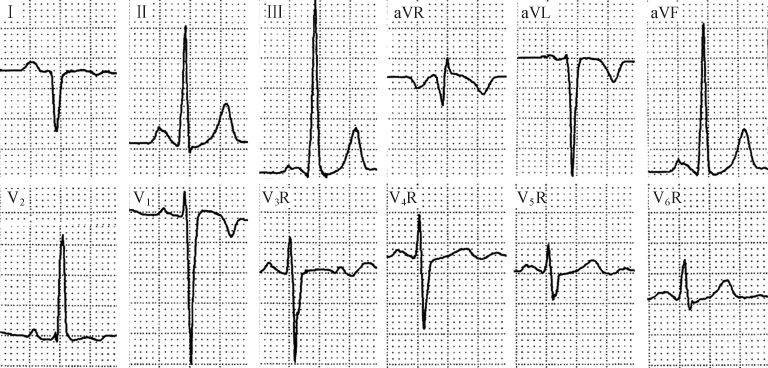
\includegraphics[width=5.1875in,height=2.47917in]{./images/Image00691.jpg}
 \captionsetup{justification=centering}
 \caption{与图\ref{fig41-8}系同一患者,对左、右手导联线反接后及右胸导联进行记录。显示肢体导联P波极性正常,但形态与上图有所不同,电轴轻度右偏,R波高电压;右胸导联显示右心室肥大,结合临床病史,提示该患者存在双心房、双心室肥大}
 \label{fig41-9}
  \end{figure} 

2.右旋心

右旋心指心脏在发育过程中下降和左旋不良,甚至右旋,使心脏不同程度地移至右侧胸腔,心尖指向右前方,但左右心房、心室的解剖关系正常,常伴有心脏其他畸形,如房间隔缺损、室间隔缺损等,不伴有内脏的转位。心电图改变有以下3个特征:

(1)各肢体导联P波极性正常。

(2)Ⅰ导联QRS、T波均倒置,而Ⅱ、Ⅲ导联QRS、T波均为正向。

(3)V\textsubscript{1} ~V\textsubscript{3}
导联QRS波群振幅增高,且呈Rs型或qR型,V\textsubscript{5}
、V\textsubscript{6} 导联R波振幅降低,且常伴有T波倒置。

\protect\hypertarget{text00050.html}{}{}

\protect\hypertarget{text00050.htmlux5cux23chapter50}{}{}

\chapter{后天性心脏病的心电图改变}

\protect\hypertarget{text00050.htmlux5cux23subid586}{}{}

\section{冠心病}

冠心病可分为隐匿型、心绞痛型、心肌梗死型、心力衰竭和心律失常型及猝死型5种类型,但这5种类型可以同时出现。

\protect\hypertarget{text00050.htmlux5cux23subid587}{}{}

\subsection{隐匿型冠心病}

隐匿型冠心病亦称为无症状型冠心病。患者虽无临床症状,但静息时或运动试验后ST段呈缺血型压低、T波低平或倒置。

\protect\hypertarget{text00050.htmlux5cux23subid588}{}{}

\subsection{心绞痛型冠心病}

有发作性胸骨后疼痛,常为一过性心肌供血不足所致。由体力劳动、运动等其他增加心肌耗氧量情况下所诱发的短暂性胸痛发作,经休息或含服硝酸甘油后,疼痛迅速缓解者,称为劳累性心绞痛;若胸痛发作与心肌耗氧量增加无明显关系,则称为自发性心绞痛,这种胸痛一般持续时间较长,程度较重,不易被硝酸甘油所缓解,但心肌酶谱正常。一般分为稳定型心绞痛、不稳定型心绞痛、变异型心绞痛及混合型心绞痛4种类型。

1.稳定型心绞痛

(1)基本概念:稳定型心绞痛又称为典型心绞痛,在3个月内,心绞痛发作的诱因、次数、疼痛性质和程度及持续时间均无明显变化者。

(2)心电图特征:心绞痛发作时,立即出现下列一项或数项改变,症状缓解后,马上恢复原状:①缺血型ST段改变:缺血部位所对应的导联ST段呈水平型、下斜型压低≥0.1mV(图\ref{fig42-1});若原有ST段压低,则在原有基础上再下降≥0.1mV;若原有ST段抬高,则ST段可回复到正常或程度减轻,出现“伪善性”改变而易被误诊;有时ST段可呈水平型延长>0.16s。②T波改变:有ST段压低的导联会出现一过性T波低平、双相或倒置,甚至出现“冠状T波”。③一过性Q-T间期延长。④U波改变:左胸导联U波倒置,偶见U波振幅增高。⑤一过性心律失常:以室性早搏多见。⑥V\textsubscript{1}
Ptf负值增大。

\begin{figure}[!htbp]
 \centering
 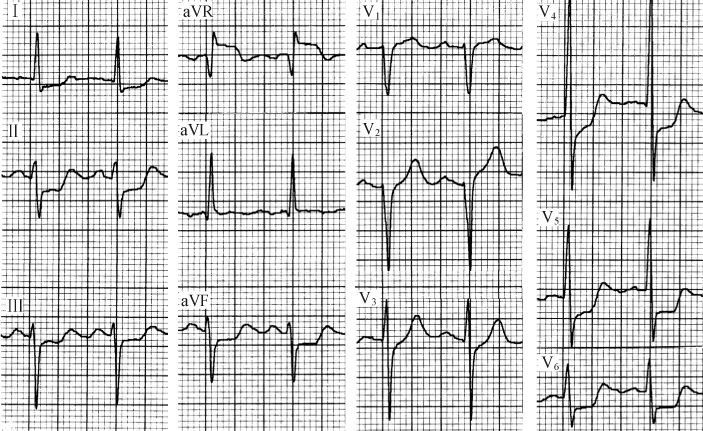
\includegraphics[width=4.75in,height=2.90625in]{./images/Image00692.jpg}
 \captionsetup{justification=centering}
 \caption{男性,69岁,胸痛发作数分钟。显示窦性心动过速、左前分支阻滞、下壁及前侧壁ST段呈缺血型改变(压低0.1~0.4mV);冠状动脉造影显示右冠状动脉近乎全部阻塞、左前降肢95\%狭窄}
 \label{fig42-1}
  \end{figure} 

2.不稳定型心绞痛

(1)基本概念:不稳定型心绞痛是指近3个月内心绞痛发作的诱因有明显变化(活动耐量减少)、发作次数增加、疼痛性质改变和持续时间延长,是介于稳定型心绞痛与急性心肌梗死之间的过渡类型。

(2)类型:①进行性心绞痛:指同等程度劳累所诱发心绞痛发作次数、程度及持续时间进行性加重,又称为恶化型劳累性心绞痛;②新发的心绞痛:指近3个月内出现的心绞痛;③中间型心绞痛:指近1个月内病情恶化,疼痛剧烈,反复发作,硝酸甘油不能缓解,但心肌酶谱正常;④心肌梗死后心绞痛:指急性心肌梗死后1个月内发生的心绞痛。

(3)心电图特征:①R波振幅可突然降低或增高,与以前图形不相符合。②ST-T改变:可出现缺血性ST-T改变,表现为ST段呈缺血型压低、T波倒置;亦可出现损伤型ST-T改变,表现为ST段呈损伤型抬高、T波高耸。③一过性心律失常:以室性早搏多见。④左胸导联U波倒置。⑤如病情进一步发展而发生急性心肌梗死,其梗死部位与原不稳定型心绞痛发作时ST-T改变的导联所反映的部位相一致。

3.变异型心绞痛

(1)基本概念:变异型心绞痛是指心绞痛发作与心肌耗氧量增加无明显关系,主要由冠状动脉一过性痉挛引起急性心肌缺血、透壁性损伤,出现损伤性ST段抬高和T波高耸。该心绞痛发作往往无明确诱因,有定时发作倾向,以夜间、凌晨多见,发作时疼痛程度较重、持续时间较长,含服硝酸甘油不能缓解,而用钙离子拮抗剂防治效果好。属自发性心绞痛范畴。

(2)心电图特征:①ST段呈损伤型抬高:面对缺血区导联ST段抬高≥0.2mV,而对应导联ST段压低;若原有ST段压低,则可出现“伪善性”改变而易误诊。②T波高耸:ST段抬高导联T波直立高耸(图\ref{fig42-2}、图\ref{fig42-3});若原有T波倒置,则可出现T波直立或倒置程度减轻而呈“伪善性”改变。③出现急性损伤阻滞图形:其特征是QRS波群时间增宽、室壁激动时间延长及R波振幅增高和S波变浅。④一过性心律失常:若急性心肌缺血、透壁性损伤发生在前壁,则以室性心律失常多见;若发生在下壁,则以房室传导阻滞多见(图\ref{fig42-4})。⑤左胸导联U波倒置,偶见U波振幅增高。⑥一部分患者可出现QRS、ST、T等波段电交替现象。⑦疼痛缓解后,上述图形改变可恢复原状,若进一步发展为心肌梗死,则梗死部位与ST段抬高、T波高耸的导联相吻合。

\begin{figure}[!htbp]
 \centering
 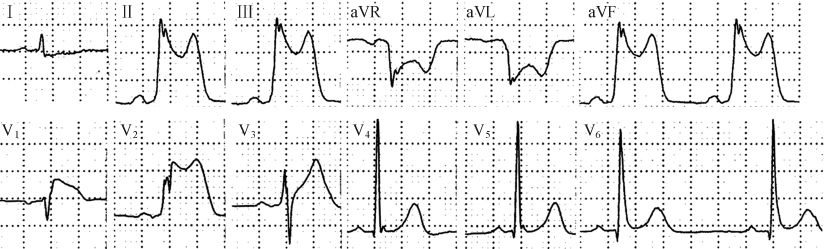
\includegraphics[width=5.5625in,height=1.67708in]{./images/Image00693.jpg}
 \captionsetup{justification=centering}
 \caption{冠心病患者,模拟12导联动态心电图显示变异型心绞痛发作时出现窦性心动过缓、下壁及前间壁ST段损伤型抬高及T波高耸、QRS波群时间增宽(0.11s)}
 \label{fig42-2}
  \end{figure} 

\begin{figure}[!htbp]
 \centering
 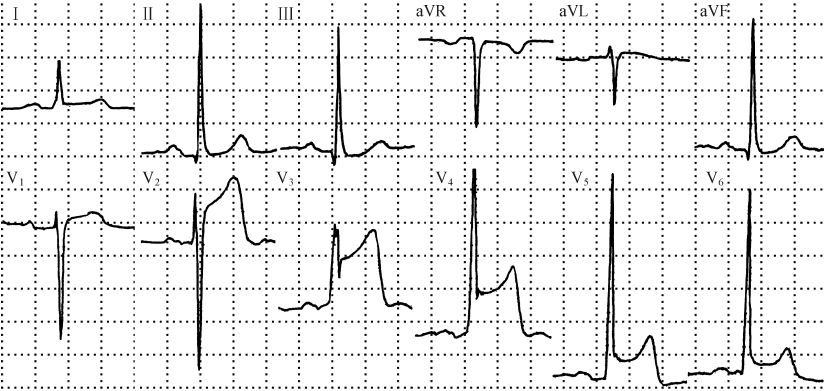
\includegraphics[width=5.5625in,height=2.63542in]{./images/Image00694.jpg}
 \captionsetup{justification=centering}
 \caption{冠心病患者,变异型心绞痛发作时出现前间壁及前侧壁ST段损伤型抬高、前间壁及前壁T波高耸、左心室高电压}
 \label{fig42-3}
  \end{figure} 

\begin{figure}[!htbp]
 \centering
 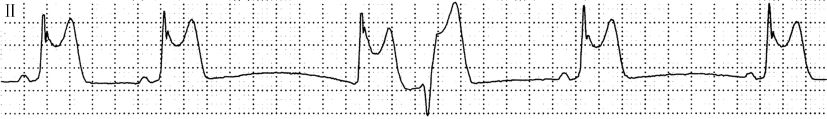
\includegraphics[width=5.58333in,height=0.80208in]{./images/Image00695.jpg}
 \captionsetup{justification=centering}
 \caption{与图\ref{fig42-2}系同一患者,除了上述改变外,尚出现窦性停搏、房室交接性逸搏、室性早搏}
 \label{fig42-4}
  \end{figure} 

4.混合型心绞痛

指患者同时存在劳累型和自发型或变异型心绞痛,即心绞痛发作时,同时存在心肌耗氧量增加和冠状动脉供血减少这两种因素参与者。

(1)劳累型合并变异型心绞痛:早已确诊为劳累型心绞痛,但近来胸痛多在夜间、凌晨发作,含服硝酸甘油不能缓解。

(2)劳累型合并自发型心绞痛:劳累后或休息时均有心绞痛发作,心电图显示缺血部位相同,白天以劳累型为主,夜间为自发型发作。

\protect\hypertarget{text00050.htmlux5cux23subid589}{}{}

\subsection{心肌梗死型冠心病}

症状多严重,由冠状动脉闭塞引起心肌急性缺血性坏死所致,心电图大多数表现为异常Q波、ST段呈损伤型抬高、T波呈缺血型倒置,其中ST-T呈动态演变是急性心肌梗死特征性改变,尤其是对非穿透性心肌梗死具有诊断价值,详见第四十四章经典的心肌梗死及其进展。

\protect\hypertarget{text00050.htmlux5cux23subid590}{}{}

\subsection{心力衰竭和心律失常型冠心病}

表现为心脏扩大、心力衰竭和心律失常,为长期心肌缺血导致心肌纤维化所致,即缺血性心肌病。详见第四十三章各类心肌病的心电图特征。

\protect\hypertarget{text00050.htmlux5cux23subid591}{}{}

\subsection{猝死型冠心病}

因原发性心脏骤停而猝死,多为缺血心肌局部发生心电紊乱,引起严重的室性心律失常所致。

\protect\hypertarget{text00050.htmlux5cux23subid592}{}{}

\subsection{平板运动试验}

1.试验方法

(1)根据年龄计算最大心率的Bruce方案,对年龄较大者采用Bruce修正方案。

(2)分极量运动试验和次极量运动试验(为最大心率的85\%~90\%)两种运动量。

2.禁忌证

(1)怀疑有急性心肌梗死。

(2)不稳定心绞痛或休息期心绞痛。

(3)已服用洋地黄类药物或低钾血症者。

(4)心电图已诊断为左心室肥大、预激综合征、左束支阻滞。

(5)严重肺部疾病、高血压者(BP>160/100mmHg)。

(6)年老体衰、行动不便者。

(7)未控制的伴有临床症状或血流动力学障碍的心律失常。

(8)临床未控制的心力衰竭。

(9)急性心肌炎、心包炎。

(10)肥厚性心肌病或其他流出道梗阻性心脏病。

(11)高度房室传导阻滞。

3.终止运动试验目标

(1)心率达到预计标准。

(2)出现典型心绞痛。

(3)ST段呈缺血型压低≥0.2mV或抬高≥0.1mV。

(4)出现严重心律失常:频发多源性及多形性室性早搏、短阵性室性心动过速、高度~三度房室传导阻滞。

(5)心率在1min内减少20次。

(6)收缩压下降10~20mmHg或收缩压上升至≥210mmHg。

(7)极度疲劳不能坚持者。

(8)出现头晕、面色苍白、步态不稳者。

4.运动过程中注意事项

(1)严格掌握好适应证、禁忌证及终止运动试验目标。

(2)必须有一定临床经验的心内科医生参与监护。

(3)配备除颤器、氧气袋(或氧气钢瓶)、注射器及相关抢救药物(肾上腺素、异丙肾上腺素、阿托品、利多卡因及硝酸甘油等。)

(4)运动过程中严密观察心电图,定期测量血压,并观察患者神态,询问患者有无不适。

(5)若出现严重反应,立即终止运动,并进行诊治或抢救。

5.运动试验阳性标准的评定

(1)运动中出现典型的心绞痛,含服硝酸甘油有效。

(2)运动中或运动后出现ST段呈缺血型压低≥0.1mV,或在原有压低基础上再下降≥0.1mV。

(3)运动中或运动后出现ST段呈损伤型抬高≥0.1mV,或在原有抬高基础上再抬高≥0.1mV。

(4)运动中或运动后出现严重心律失常:多源性室性早搏、室性心动过速、高度~三度房室传导阻滞、心房颤动、高度窦房传导阻滞。

(5)运动中或运动后出现U波倒置。

6.运动试验阳性价值的评定

(1)运动试验阳性者,约有30\%~40\%患者,经冠状动脉造影证实有病变。

(2)ST段呈缺血型压低时,若出现时间越早,则冠状动脉病变程度越严重。

(3)ST段呈缺血型压低≥0.3mV者,往往属于三支病变或左冠状动脉主干病变。

(4)ST段呈缺血型压低持续时间:运动停止后,ST段恢复时间长短亦可提示冠状动脉病变程度。若运动后立即出现ST段压低并持续时间≥8min者,多为二支、三支冠状动脉病变。

(5)运动中、后出现心绞痛、低血压,均有重要临床意义。

(6)出现U波倒置,是左冠状动脉前降支狭窄严重的标志,具有高度特异性。

7.运动试验应用价值:①冠心病的诊断;②已知或可疑冠心病患者的严重程度、危险性和预防的评价;③急性心肌梗死患者出院前早期危险性评估;④评估心脏功能。

\protect\hypertarget{text00050.htmlux5cux23subid593}{}{}

\section{高血压性心脏病}

\protect\hypertarget{text00050.htmlux5cux23subid594}{}{}

\subsection{高血压性心脏病}

1.概述

长期高血压将引起左心室收缩期负荷过重,导致左心室代偿性增厚,可显著地增加心源性猝死、心肌缺血、心力衰竭和室性心律失常等心血管意外事件的发生率和死亡率。

2.病理生理改变

长期左心室收缩期负荷过重及神经内分泌等体液因素影响,导致左心室心肌细胞增大、肌纤维增粗增长、心肌间质重构引起心肌重量和硬度增加,形成左心室代偿性肥厚,包括向心性对称性左心室肥厚、不对称性左心室肥厚及离心性左心室肥大。左心室肥厚将引起心肌缺血、室性心律失常及各种传导阻滞。

3.心电图特征

(1)左心室高电压:左胸导联或(和)肢体导联R波电压明显增高。

(2)左心室肥厚伴劳损:左胸导联、肢体导联R波电压均明显增高,QRS波群时间轻度增宽,同时伴有ST段呈缺血型压低、T波负正双相或倒置、U波负正双相或倒置(图\ref{fig42-5})。

\begin{figure}[!htbp]
 \centering
 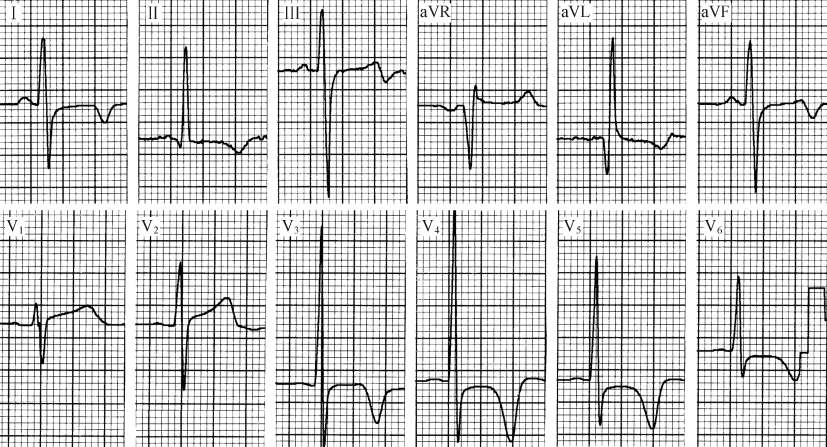
\includegraphics[width=5.58333in,height=3.02083in]{./images/Image00696.jpg}
 \captionsetup{justification=centering}
 \caption{男性,56岁,患高血压病20余年,心脏超声波显示不对称性左心室肥厚、不能排除心尖肥厚性心肌病。心电图显示左心室肥大伴劳损(V\textsubscript{1}~V\textsubscript{6} 导联定准电压均为0.5mV)}
 \label{fig42-5}
  \end{figure} 


(3)室性心律失常:以多源性室性早搏、短阵性室性心动过速多见。与下列因素有关:①左心室肥厚多伴有心内膜下心肌缺血,可强烈地刺激室性异位灶发放冲动;②心室肌不规则肥厚和局部纤维化妨碍冲动均一地传至整个心肌而引起折返活动;③肥大心肌细胞的电生理与正常细胞的电生理不同,更易引发心律失常;④交感神经系统和神经体液内分泌因子活性加强,促使心律失常的发生。

(4)传导阻滞:以左束支阻滞、左前分支阻滞及右束支阻滞多见。与左心室肥厚扩张牵拉左束支、左前分支使之受损有关,而右束支阻滞则与心室收缩时,室间隔向右侧膨出牵拉右束支使之受损有关。

\protect\hypertarget{text00050.htmlux5cux23subid595}{}{}

\subsection{高血压性心肌病}

1.基本概念

继发于高血压引起的左心室肥厚、舒张充盈受损、左心室收缩功能减退、心室电活动不稳定、冠状动脉储备下降及心肌缺血,出现以扩张型或限制型心肌病、心力衰竭为特征的特异性心肌病。

2.病理生理改变

左心室肥厚时,左心室舒张期硬度增加,心室顺应性减退,首先出现舒张功能减退,继而影响收缩功能,使左心室射血分数下降,最终导致心力衰竭,加重心肌缺血、心电紊乱和传导阻滞。

3.心电图特征

与高血压性心脏病心电图特征类似,但室性心律失常及心室内传导阻滞的发生率更高、更严重。

\protect\hypertarget{text00050.htmlux5cux23subid596}{}{}

\section{肺源性心脏病}

\protect\hypertarget{text00050.htmlux5cux23subid597}{}{}

\subsection{慢性肺源性心脏病}

1.基本概念

由支气管、肺部慢性疾病引起肺循环阻力增加、肺动脉压力升高,导致右心室肥厚、右心房扩大,最后发生右心充血性心力衰竭的一组疾病。

2.病理生理改变

长期肺动脉高压引起右心室收缩期负荷过重,首先出现右心室流出道肥厚,继之出现右心室游离壁肥厚,随着病情的发展,出现右心室和右心房扩张、心脏顺钟向转位;当病变累及传导组织时,可出现各种心律失常及传导阻滞。

3.心电图特征

(1)肺型P波:①Ⅱ、Ⅲ、aVF导联P波高耸,电压≥0.25mV;②Ⅱ、Ⅲ、aVF导联P波呈尖峰状,电压在0.20~0.24mV,P电轴>+80°;③低电压时,P波呈尖峰状,其振幅>$\frac{1}{2}$
R,P电轴>+80°。符合以上P波改变之一者,均可诊断为肺型P波(图\ref{fig42-6})。

\begin{figure}[!htbp]
 \centering
 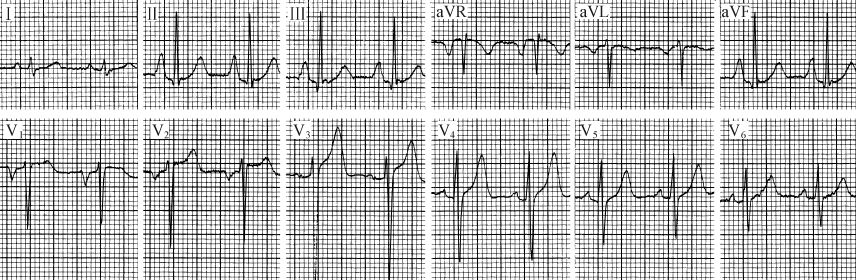
\includegraphics[width=5.78125in,height=1.88542in]{./images/Image00697.jpg}
 \captionsetup{justification=centering}
 \caption{慢性肺源性心脏病患者出现肺型P波、V\textsubscript{1}Ptf值增大、顺钟向转位}
 \label{fig42-6}
  \end{figure} 


(2)V\textsubscript{1}
导联P波呈正负双相型或直立尖角型:呈正负双相型时,正相波振幅乘以时间,代表右心房除极向量面积,主要反映右心房结构和功能。当该面积≥+0.03mm·s时,肺心病诊断的敏感性约57\%,特异性90\%;部分患者负相波表现为深而窄,V\textsubscript{1}
Ptf值增大≥|-0.04mm·s|。

(3)心电轴右偏≥+90°或出现S\textsubscript{Ⅰ} S\textsubscript{Ⅱ}
S\textsubscript{Ⅲ} 综合征,呈假性电轴左偏。

(4)aVR导联QRS波群R/S或R/Q>1。

(5)胸前导联出现重度顺钟向转位:V\textsubscript{1} ~V\textsubscript{6}
导联QRS波群均呈rS型,r/S<1,或V\textsubscript{5} 、V\textsubscript{6}
导联呈RS型,R/S<1或S>$\frac{1}{2}$ R。

(6)右胸导联出现异常Q波:有时V\textsubscript{1} ~V\textsubscript{3}
导联QRS波群呈QS、Qr、qr或qR型,约占12\%。

(7)V\textsubscript{1} 导联R/S>1,R波电压>1.0mV或呈qR型。

(8)R\textsubscript{V\textsubscript{1}}
+S\textsubscript{V\textsubscript{5}}
≥1.2mV:R\textsubscript{V\textsubscript{1}}
电压增高反映了右心室游离壁肥厚引起的向前向量增大,而S\textsubscript{V\textsubscript{5}}
增深,则反映了右心室流出道肥厚引起的向右后向量增大。这一诊断指标,敏感性约为27\%,而特异性高达100\%。

(9)QRS波群低电压:每个肢体导联QRS波群R+S电压<0.5mV或每个胸前导联R+S电压<1.0mV。

(10)心律失常:以窦性心动过速、多源性房性早搏、短阵性房性心动过速及室性早搏多见。

(11)右束支阻滞。

(12)非特异性ST-T改变:多见于下壁导联与右胸导联。

慢性肺源性心脏病除了右心室肥厚外,还兼有右心房扩大、顺钟向转位及肺气肿。故除了一般右心室肥厚心电图特征外,肺型P波、重度顺钟向转位、低电压是其特征性改变,可根据这3个特征性改变加上右心室肥厚图形,便可确立其诊断。

4.预后判断的心电图指标

(1)心率、Ⅱ导联及aVF导联P波振幅:这三项指标的数值越大,预后越差。

(2)V\textsubscript{1}
导联QRS波群呈qR型,是严重肺心病的特征性改变,提示预后不良。

\protect\hypertarget{text00050.htmlux5cux23subid598}{}{}

\subsection{肺栓塞(急性肺源性心脏病)}

1.基本概念

急性肺栓塞是指肺动脉某支血管内突然发生血源性阻塞,引起肺动脉反射性痉挛,导致右心室急剧扩张和急性右心衰竭,严重者可发生休克或猝死,又称为急性肺源性心脏病。临床上约50\%患者出现具有诊断意义的心电图特征,但应密切结合临床。

2.病理生理改变

肺动脉突然栓塞及同时出现的神经体液异常,导致肺动脉压力骤然升高,引起急性右心室收缩期负荷增加,右心室和右心房扩张,心脏顺钟向转位,出现右心室劳损和右心房扩大图形。此外,右心室壁张力增高可引起局部心肌缺血,出现ST-T改变。

3.心电图特征(图\ref{fig42-7})

\begin{figure}[!htbp]
 \centering
 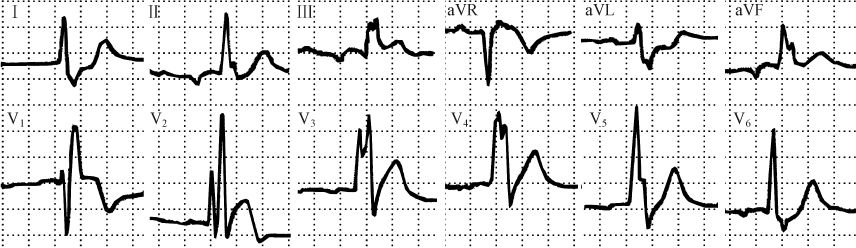
\includegraphics[width=5.78125in,height=1.67708in]{./images/Image00698.jpg}
 \captionsetup{justification=centering}
 \caption{多发性骨折、急性肺栓塞患者出现加速的房性逸搏心律、新发的完全性右束支阻滞、S\textsubscript{Ⅰ}Q\textsubscript{Ⅲ} 型、非特异性ST-T改变(引自刘子荣)}
 \label{fig42-7}
  \end{figure} 


(1)窦性心动过速:为最常见的心律失常,心率多在100~125次/min,临床上若心率>90次/min,即对诊断有帮助。

(2)肺型P波、PR段压低:Ⅱ导联P波电压≥0.25mV,可能与右心房负荷过重、右心房扩大及心动过速有关。约1/3患者出现PR段压低。

(3)S\textsubscript{Ⅰ} Q\textsubscript{Ⅲ} T\textsubscript{Ⅲ}
型或S\textsubscript{Ⅰ} Q\textsubscript{Ⅲ}
型:即Ⅰ导联出现较明显的S波(>0.15mV),Ⅲ导联出现较明显的Q波(多呈QR型、qR型,其时间多<0.04s,深度<
$\frac{1}{4}$
R)伴T波倒置,为常见而重要的心电图特征。反映了急性右心室扩张和(或)一过性左后分支阻滞。

(4)电轴偏移:可发生右偏(+90°~+100°或较发病前右偏20°以上)或左偏。

(5)重度顺钟向转位:移行区左移至V\textsubscript{5}
导联或V\textsubscript{1} ~V\textsubscript{6} 导联均呈rS型。

(6)新出现的右束支阻滞:呈不完全性或完全性右束支阻滞图形。

(7)非特异性ST-T改变:Ⅰ、Ⅱ、V\textsubscript{5} 、V\textsubscript{6}
导联ST段轻度压低,Ⅲ、aVR、V\textsubscript{1} ~V\textsubscript{3}
导联ST段呈弓背向上型轻度抬高;V\textsubscript{1} ~V\textsubscript{3}
导联T波倒置,若呈对称性倒置,则见于大块肺栓塞的早期(24h内)。

(8)可出现各种房性心律失常:以心房颤动、扑动多见,常为一过性。

4.鉴别诊断

因急性肺栓塞临床上可出现胸痛、呼吸困难,心电图出现S\textsubscript{Ⅰ}
Q\textsubscript{Ⅲ} T\textsubscript{Ⅲ} 型及V\textsubscript{1}
~V\textsubscript{3}
导联ST段抬高、T波倒置,应与急性下壁、前间壁心肌梗死相鉴别。

\protect\hypertarget{text00050.htmlux5cux23subid599}{}{}

\section{风湿性心脏病}

\protect\hypertarget{text00050.htmlux5cux23subid600}{}{}

\subsection{二尖瓣狭窄}

1.病理生理改变

正常成人二尖瓣口直径约为3~3.5cm,面积约为4~6cm\textsuperscript{2}
。当二尖瓣口狭窄到一定程度时(约1/2),可引起左心房压力增高、代偿性扩大,继之出现肺静脉、肺毛细血管压力升高导致肺淤血和肺动脉压力增高,从而引起右心室肥大、扩张。

2.心电图表现

(1)二尖瓣型P波及V\textsubscript{1}
Ptf负值增大:与左心房扩大及心房内传导延缓有关。

(2)右心室肥大的心电图特征。

(3)可出现肺型P波:与右心房负荷过重、扩大有关。

(4)心律失常:①房性心律失常:早期以多源性房性早搏、短阵性房性心动过速多见,晚期几乎都有心房扑动、颤动发作,且以后者多见;②室性心律失常:以多源性、多形性室性早搏多见,可见短阵性室性心动过速,多与洋地黄毒性作用、低钾血症等因素有关。

(5)传导阻滞:以房室传导阻滞、束支阻滞多见。

\protect\hypertarget{text00050.htmlux5cux23subid601}{}{}

\subsection{二尖瓣关闭不全}

1.病理生理改变

二尖瓣关闭不全时,部分血液在左心室收缩时返流到左心房,引起左心房和左心室的容量增大,从而导致左心房、左心室肥大或扩张。

2.心电图表现

(1)二尖瓣型P波及V\textsubscript{1} Ptf负值增大。

(2)左心室肥大:左胸导联R波电压增高,T波高耸,表现为舒张期负荷过重的心电图特征。

(3)可出现各种心律失常及传导阻滞。

\protect\hypertarget{text00050.htmlux5cux23subid602}{}{}

\subsection{二尖瓣狭窄伴关闭不全}

二尖瓣狭窄伴关闭不全,表现为左心房和左心室的舒张期容量负荷增大及右心室的收缩期负荷过重,严重者可出现双心房、双心室肥大的心电图特征(图\ref{fig42-8})。

\begin{figure}[!htbp]
 \centering
 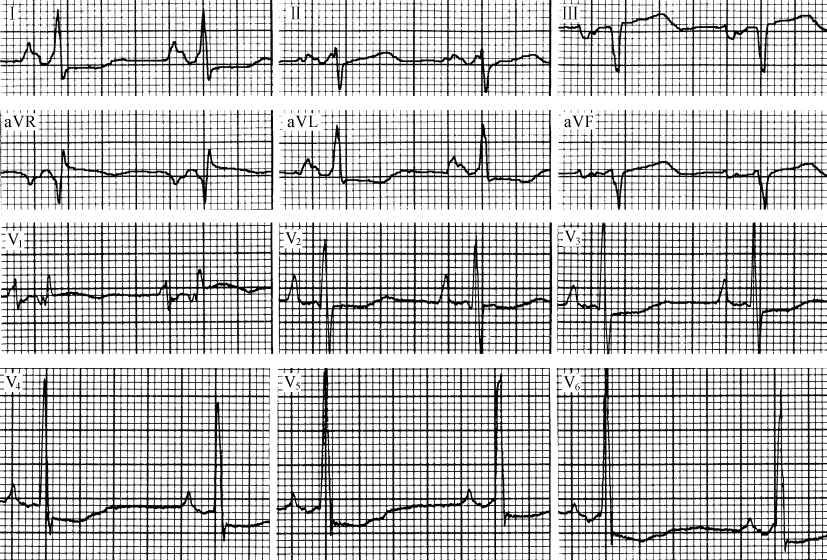
\includegraphics[width=5.58333in,height=3.78125in]{./images/Image00699.jpg}
 \captionsetup{justification=centering}
 \caption{风心病、二尖瓣狭窄伴关闭不全患者,出现双心房肥大、局限性前间壁异常Q波、电轴左偏、提示双心室肥大伴劳损、高侧壁及前侧壁ST-T改变}
 \label{fig42-8}
  \end{figure} 

\protect\hypertarget{text00050.htmlux5cux23subid603}{}{}

\subsection{主动脉瓣狭窄}

正常主动脉瓣口面积为3cm\textsuperscript{2}
。当瓣口面积<1cm\textsuperscript{2}
时,左心室射血受阻,收缩期负荷过重,心搏出量减少,收缩期末左心室残余血量增加,舒张期血液充盈量增加,出现代偿性肥厚,最后发生左心衰竭。心电图上可出现左心室肥厚伴劳损改变及室性心律失常、左前分支阻滞或左束支阻滞(可掩盖左心室肥厚图形)。

\protect\hypertarget{text00050.htmlux5cux23subid604}{}{}

\subsection{主动脉瓣关闭不全}

主动脉瓣关闭不全时,左心室舒张期同时接受来自左心房流入的血液和从主动脉返流回来的血液,故左心室舒张期容量负荷明显增加,导致左心室肥大、扩张。心电图表现为左心室肥大、电轴左偏、T波高耸,呈现舒张期负荷过重的特征。

\protect\hypertarget{text00050.htmlux5cux23subid605}{}{}

\section{甲状腺功能紊乱性心脏病}

\protect\hypertarget{text00050.htmlux5cux23subid606}{}{}

\subsection{概述}

甲状腺功能紊乱性心脏病包括功能亢进引起的心脏病和功能减退引起的心脏病。

\protect\hypertarget{text00050.htmlux5cux23subid607}{}{}

\subsection{甲状腺功能亢进性心脏病}

1.病理生理改变

甲状腺功能增强,分泌甲状腺素过多,一方面引起代谢亢进,增加心脏负荷,另一方面甲状腺素直接作用于心肌和周围血管,并加强儿茶酚胺作用,导致心率加快、心脏肥大、心肌耗氧量增加及心房肌兴奋性增高、不应期缩短。

2.心电图表现

(1)窦性心动过速:心率多在120次/min左右,系甲状腺素毒性作用和交感神经兴奋性增高所致。

(2)心脏肥大:可表现为右心房、右心室、左心室或全心肥大的心电图特征。

(3)非特异性ST-T改变。

(4)心律失常:以房性早搏、短阵性房性心动过速及心房颤动多见,与甲状腺素使心房肌兴奋性增高,不应期缩短有关。尚可出现房室传导阻滞、束支阻滞,与低钾血症、传导组织局灶性坏死和纤维化有关。

3.甲状腺功能亢进性心肌病

(1)基本概念:当甲状腺功能亢进患者出现以心脏扩大、心力衰竭和心房颤动为主要特征时,便可称为甲状腺功能亢进性心肌病。与甲状腺素毒性作用、长期心动过速或心房颤动有关。经治疗后,上述心脏异常可消失或明显好转。

(2)诊断标准:①甲状腺功能亢进诊断明确;②有心脏扩大或心力衰竭或心绞痛或明显心律失常或二尖瓣脱垂伴杂音之一者;③经治疗后,心脏异常改变消失或明显好转;④除外其他器质性心脏病。

4.可能由甲状腺功能亢进引起的心血管异常改变

(1)原因不明的阵发性或持续性心房颤动,心室率快而不易被洋地黄类药物所控制。

(2)原因不明的右心衰竭,但患者无贫血、发热或脚气病等,洋地黄类药物疗效不佳。

(3)无法解释的心动过速。

(4)血压波动而脉压差增大者。

(5)器质性心脏病患者发生心力衰竭时,常规治疗疗效不佳或心率增快难以控制者。

\protect\hypertarget{text00050.htmlux5cux23subid608}{}{}

\subsection{甲状腺功能减退性心脏病}

1.病理生理改变

甲状腺素分泌不足,机体基础代谢率低下,心肌能量代谢及心肌对儿茶酚胺敏感性均降低,心肌可发生非特异性病理改变,导致心率减慢,心搏出量减少及心脏扩大;毛细血管通透性增加、嗜水性粘多糖和粘蛋白堆积,出现心包积液;血中胆固醇增高,易发生动脉粥样硬化。

2.心电图表现

(1)窦性心动过缓。

(2)出现各种传导阻滞:房室传导阻滞、束支阻滞及不定型心室内传导阻滞。

(3)QRS波幅低电压。

(4)非特异性ST-T改变及Q-T间期延长。

\protect\hypertarget{text00050.htmlux5cux23subid609}{}{}

\section{心肌炎}

1.概述

心肌炎可由感染性(病毒、细菌、支原体等微生物感染)、过敏或变态反应、化学、物理或药物等因素引起心肌内局部性或弥漫性炎症性病变。以病毒性心肌炎多见,临床上诊断比较困难,需要心肌活检才能确诊。心电图检查对心肌炎的诊断具有一定的价值,并能指导制订治疗方案和判断预后。

2.分型

临床上最常见的病毒性心肌炎可分为3型。

(1)急性心肌炎:以心肌炎症、损伤为主,无或仅有轻微纤维化;临床上短时间内发生心力衰竭和各种心律失常、传导阻滞,多在6个月内死亡或痊愈。

(2)亚急性心肌炎:有少量心肌损害灶,出现广泛的心肌纤维化和愈合性心肌损害灶;临床上可交替出现心功能代偿和心力衰竭,多伴心律失常及传导阻滞,病程6个月至数年。

(3)慢性心肌炎:病程缓慢,达3~5年以上;临床上表现为心脏肥大、扩张,可遗留程度不等的心力衰竭症状及各种心律失常、传导阻滞。

3.心电图表现

(1)窦性心律失常:以窦性心动过速多见,若炎症累及窦房结,则可出现显著的窦性心动过缓、窦房传导阻滞、窦性停搏,表现为病窦综合征。

(2)传导阻滞:以一度、二度房室传导阻滞、心室内传导阻滞多见,大多数是可逆性的,约有30\%患者迅速发展为三度房室传导阻滞。

(3)心律失常:以房性、室性早搏及短阵性房性、室性心动过速多见。

(4)QRS波幅低电压:约占12\%。

(5)Q-T间期延长:约占30\%。

(6)非特异性ST-T改变。

(7)少数重症心肌炎患者可出现异常Q波、ST段呈损伤型抬高酷似急性心肌梗死图形,预示心肌损害较严重。

4.急性病毒性心肌炎心电图诊断标准

急性上呼吸道、消化道感染后1~3周内新出现下列心电图改变:

(1)房室或窦房传导阻滞、束支阻滞。

(2)两个以上导联ST段呈缺血性压低>0.05~0.1mV或多个导联ST段异常抬高或有异常Q波。

(3)频发多形性、多源性、成对早搏或并行性早搏,短阵性房性、室性心动过速等。

(4)两个以上以R波为主的导联T波低平或倒置。

(5)频发房性早搏或室性早搏。

具有(1)~(3)任何一项,即可考虑诊断急性病毒性心肌炎;具有(4)或(5)项,无明显病毒感染史者,要补充左心室收缩功能减弱、病程早期有心肌酶谱增高这两个条件。

\protect\hypertarget{text00050.htmlux5cux23subid610}{}{}

\section{心包炎}

\protect\hypertarget{text00050.htmlux5cux23subid611}{}{}

\subsection{急性心包炎}

急性心包炎除了心包脏层和壁层间的渗出性炎症外,心包下的心外膜心肌也受到波及而发生弥漫性炎症性反应,出现损伤性改变和缺血性改变;若心包内有积液,则心肌产生的电流会发生短路现象。

1.心电图特征

(1)窦性心动过速。

(2)广泛导联ST段呈凹面向上型抬高:发病早期,即胸痛发生后数小时,Ⅰ、Ⅱ、aVF、V\textsubscript{2}
~V\textsubscript{6}
导联ST段呈凹面向上型抬高,一般<0.5mV,以Ⅱ、V\textsubscript{5}
、V\textsubscript{6} 导联为明显,aVR、V\textsubscript{1}
导联ST段压低,持续数小时至数天,便回到等电位线。与炎症累及心外膜下浅层心肌产生损伤性电流有关(图\ref{fig42-9})。

\begin{figure}[!htbp]
 \centering
 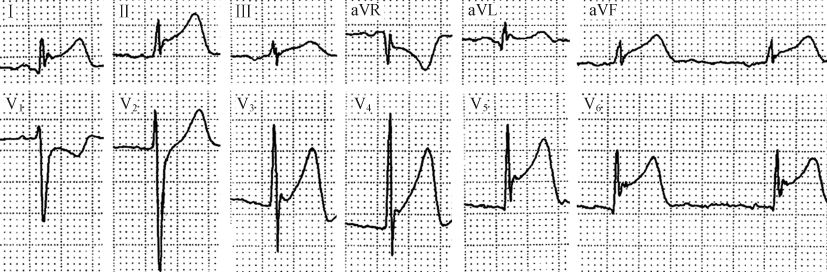
\includegraphics[width=5.58333in,height=1.83333in]{./images/Image00700.jpg}
 \captionsetup{justification=centering}
 \caption{男性,17岁,发热、胸痛,临床诊断为急性心包炎、心肌炎。显示窦性心动过缓伴P电轴左偏、P波低电压、高侧壁及下壁和前侧壁ST段抬高伴T波高耸酷似变异型心绞痛的心电图改变}
 \label{fig42-9}
  \end{figure} 

(3)T波改变:以R波为主的导联T波低平或倒置(<0.5mV),多发生在ST段回到等电位线后。与心外膜下心肌缺血有关。

(4)PR段偏移:PR段偏移方向与ST段偏移方向相反,即ST段抬高导联,其PR段多呈水平型压低0.05~0.15mV。PR段偏移发生在急性心包炎早期,可早于ST段抬高,甚至是唯一表现,具有早期特异性诊断价值。与心房肌较薄,较易损伤引起心房复极异常有关。

(5)QRS波幅低电压:与心包积液有关。

(6)偶尔可见QRS、ST、T等波段电交替现象。

2.分期

急性心包炎典型的心电图改变,可分为4期:①Ⅰ期:主要是PR段压低和ST段抬高,这两者具有特征性改变,具有诊断价值;②Ⅱ期:ST段回到基线;③Ⅲ期:T波倒置;④Ⅳ期:T波回到基线(表42-1)。

\begin{table}[htbp]
\centering
\caption{急性心包炎心电图改变}
\label{tab42-1}
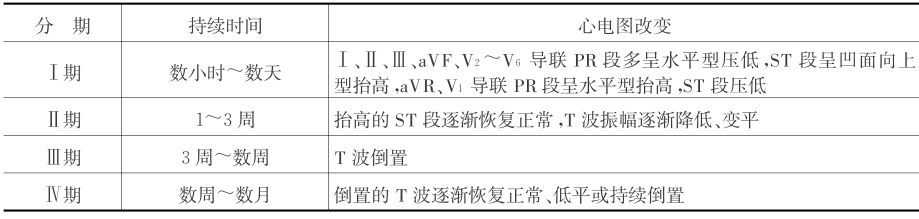
\includegraphics[width=6.20833in,height=1.47917in]{./images/Image00701.jpg}
\end{table}

3.鉴别诊断

急性心包炎患者早期有胸痛、ST段呈凹面向上型抬高,需与急性心肌梗死、早复极综合征相鉴别(表42-2)。

\begin{table}[htbp]
\centering
\caption{急性心包炎与急性心肌梗死、早复极综合征的心电图鉴别}
\label{tab42-2}
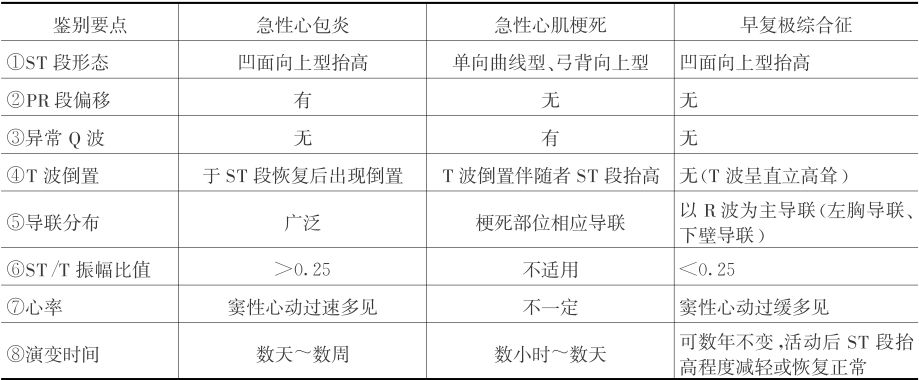
\includegraphics[width=6.20833in,height=2.5625in]{./images/Image00702.jpg}
\end{table}

\protect\hypertarget{text00050.htmlux5cux23subid612}{}{}

\subsection{慢性心包炎}

1.病理生理改变

心包膜纤维组织广泛增生、增厚及粘连,妨碍心脏收缩和舒张功能,尤其是左心室舒张受限,导致左心房、肺静脉压力增高,引起肺动脉高压和右心室肥大;心包腔内积液,造成心脏电流传导短路现象及受压的心肌细胞萎缩,可出现QRS波幅低电压;心包炎可引起心肌病变及缺血,出现ST-T改变。

2.心电图表现

(1)窦性心动过速:心率100~160次/min多见,与心脏收缩和舒张功能受限,心排出量减少后一种代偿性反应有关。

(2)QRS波幅低电压。

(3)广泛导联ST-T改变:以R波为主的导联ST段压低、T波低平或倒置。

(4)P波改变:可出现P波增高、增宽及双峰切迹,与心房肌受累、心房扩大或心房内传导阻滞有关。

(5)房性心律失常:可出现房性早搏、短阵性房性心动过速、心房颤动等,与心房肌受累及心房内压力长期增高有关。

(6)病程较长者,可出现右心室肥大、右束支阻滞(图\ref{fig42-10})。

\begin{figure}[!htbp]
 \centering
 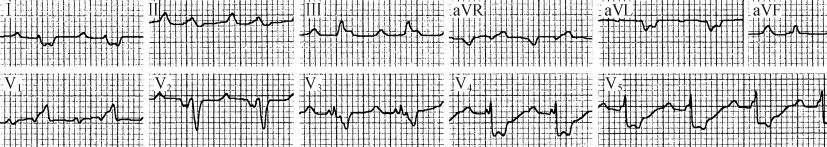
\includegraphics[width=5.58333in,height=0.98958in]{./images/Image00703.jpg}
 \captionsetup{justification=centering}
 \caption{慢性心包炎患者出现窦性心动过速、肺型P波、低电压、完全性右束支阻滞、前间壁异常Q波、顺钟向转位、右心室肥大}
 \label{fig42-10}
  \end{figure} 

\protect\hypertarget{text00050.htmlux5cux23subid613}{}{}

\subsection{心包积液}

大量心包积液时,心电图上可出现窦性心动过速、低电压、广泛导联T波改变及P、QRS、T各波段电交替现象。在肯定有心包积液情况下,电交替现象提示有大量心包积液或心包填塞。

\protect\hypertarget{text00051.html}{}{}

\protect\hypertarget{text00051.htmlux5cux23chapter51}{}{}

\chapter{各类心肌病的心电图改变}

\protect\hypertarget{text00051.htmlux5cux23subid614}{}{}

\subsection{基本概念和分类}

1996年世界卫生组织(WHO)和国际心脏病学会(FSH)将心肌病定义为心肌病变伴心功能障碍的疾病,并将其分为原发性心肌病和特异性(继发性)心肌病两种,前者包括扩张型、肥厚型、限制型、致心律失常性右室心肌病和未分类心肌病,后者指继发于已明确病因的心肌疾病,如缺血性心肌病、瓣膜性心肌病、高血压性心肌病、炎症性心肌病、代谢性心肌病、酒精性心肌病、围生期心肌病、糖尿病性心肌病、克山病、家族遗传性心肌病、心动过速性心肌病等。这类患者临床特征为进行性心脏扩大、心功能减退及各种心律失常和传导障碍,病理特征为弥漫性心肌退行性变及纤维化,心室肥厚扩张。临床上以扩张型心肌病最为常见,其次为肥厚型心肌病;而心电图改变以肥厚型心肌病最具特征性,其次为致心律失常性右室心肌病。

2006年美国心脏病协会对心肌病重新进行了定义和分类,将离子通道疾病如长Q-T间期综合征、短Q-T间期综合征、Brugada综合征、异常J波、Lenegre综合征及儿茶酚胺介导的心动过速等原发性心电活动异常疾病归入心肌病范畴;把由其他心血管疾病所致的心肌病理改变不包括在心肌病范畴,如心脏瓣膜病、高血压性心脏病、先天性心脏病、冠心病等所致心肌病,建议不再使用“缺血性心肌病”这一命名。仍将心肌病分为原发性心肌病和继发性心肌病两大类。原发性心肌病是指病变仅局限在心肌,根据发病机制可分为遗传性、混合性及获得性3种。遗传性心肌病包括肥厚型心肌病、致心律失常性右室心肌病、左心室致密化不全、线粒体肌病和离子通道病等;混合性心肌病包括扩张型和限制型心肌病;获得性心肌病包括炎症性心肌病、应激性心肌病、围生期心肌病、心动过速性心肌病、酒精性心肌病等。继发性心肌病是指心肌的病变为全身多器官病变的一部分,心脏受累的程度变化很大,包括淀粉样变性心肌病、糖尿病性心肌病、糖原蓄积所致的心肌病、脚气病性心肌病等。

\protect\hypertarget{text00051.htmlux5cux23subid615}{}{}

\subsection{扩张型心肌病}

1.基本概念

扩张型心肌病是指由原发性或混合性心肌疾病导致一侧或双侧心腔扩大,继以心室收缩功能减退的原因不明的心肌病,约30\%~50\%患者具有家族遗传特点,常伴有骨骼肌和神经肌肉病变。

2.病理生理改变

心肌细胞肥大、纤维组织增生,并出现非特异性退行性改变及间质纤维化;病变弥散,波及全心,但以左心室扩张为主,心室壁肥厚相对不明显甚至变薄;心脏收缩功能减退,心排血量减少引起心力衰竭。病变累及传导组织可引起各种心律失常和传导障碍。附壁血栓脱落可引起心、脑、肾等重要器官栓塞。

3.心电图改变

几乎所有病例都有心电图异常改变,以异位搏动和异位心律最为常见,其次为传导阻滞和STT改变(图\ref{fig43-1}、图\ref{fig43-2})。

\begin{figure}[!htbp]
 \centering
 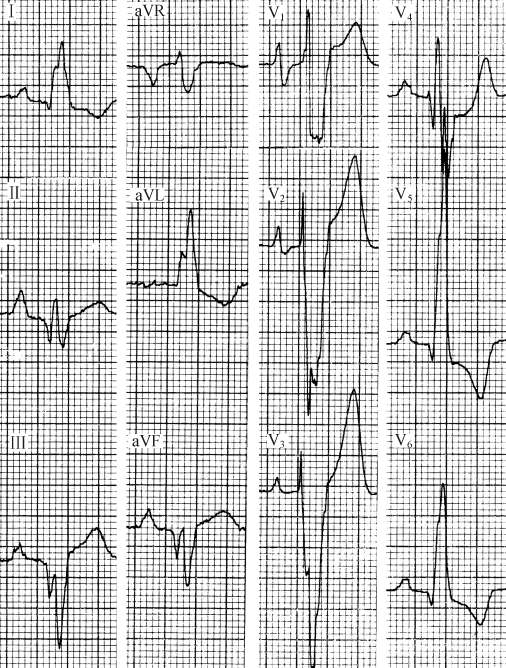
\includegraphics[width=3.41667in,height=4.51042in]{./images/Image00704.jpg}
 \captionsetup{justification=centering}
 \caption{男性,38岁,扩张型心肌病。心电图显示右心房肥大、V\textsubscript{1}Ptf增大(提示左心房负荷过重)、左心室肥大伴劳损、不定型心室内传导阻滞(QRS时间0.20s)、下壁异常Q波}
 \label{fig43-1}
  \end{figure} 


\begin{figure}[!htbp]
 \centering
 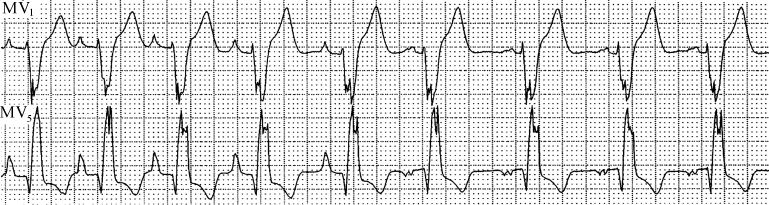
\includegraphics[width=5.19792in,height=1.38542in]{./images/Image00705.jpg}
 \captionsetup{justification=centering}
 \caption{男性,68岁,扩张型心肌病。显示非阵发性房性心动过速(70~85次/min)、右心房肥大、完全性左束支阻滞、异常Q波(MV\textsubscript{1}导联定准电压0.5mV)}
 \label{fig43-2}
  \end{figure} 


(1)异位搏动和异位心律:90\%的患者有复杂性室性心律失常,如多源性和(或)多形性室性早搏、成对室性早搏、短阵性室性心动过速等,10\%~20\%的患者出现房性心律失常,如房性早搏、短阵性房性心动过速及心房颤动等。有时,一些顽固性、难治性心律失常可能是扩张性心肌病早期诊断的重要线索。

(2)传导阻滞:最常见的是房室传导阻滞,以二度、三度阻滞多见,阻滞部位多在希氏束分叉以下,其次为不定型心室内传导阻滞、束支阻滞、双分支或三分支阻滞。传导阻滞的出现与病变累及传导系统及继发于心脏扩大,导致希-浦系统广泛受损有关。

(3)左心室高电压:约10\%的患者出现左心室高电压,其发生率低与心室以扩张为主而心室壁增厚不明显有关。

(4)QRS波幅低电压:约占15\%,与心肌细胞退行性变、坏死、纤维化导致心室除极时所产生的电位减少有关。

(5)异常Q波:约占11\%~20\%,常见于左胸导联及肢体导联,与心肌细胞片状坏死、疤痕形成(纤维化)有关。出现异常Q波,意味着心肌有较严重的病理学改变。

(6)非特异性ST-T改变:约占40\%~50\%,以R波为主导联ST段呈水平型或下斜型压低,T波低平、负正双相或倒置。

(7)Q-T间期延长:约占20\%,与心室除极、复极时间延长有关。

(8)P波时间增宽:约占20\%,与左心房负荷过重、扩大及左心房传导延缓有关。

4.易引发猝死的心电图表现

(1)多源性成对室性早搏、短阵性或持续性室性心动过速伴心室晚电位阳性者。

(2)不定型心室内传导阻滞、双分支阻滞及三分支阻滞。

\protect\hypertarget{text00051.htmlux5cux23subid616}{}{}

\subsection{肥厚型心肌病}

1.基本概念

肥厚型心肌病是指原因不明的左心室心肌不对称、不均匀性肥厚,心室腔变小,以左心室血液充盈受阻及舒张期顺应性降低为基本病变的心肌病。约50\%的患者具有家族遗传特点,由基因突变导致肌节功能异常所致,为常染色体显性遗传的家族遗传性疾病。

2.病理生理改变

心室肌纤维肥大,排列紊乱,病变主要累及室间隔和左心室,导致室间隔呈显著不对称性肥厚、左心室游离壁部分或全部非对称性或弥漫性肥厚,前者出现左心室流出道狭窄而成为梗阻型心肌病。心肌细胞间质纤维化、结缔组织增生,心室僵硬度增高,左心室舒张功能受损导致舒张期顺应性明显降低。由于心室腔变小,舒张期顺应性降低,左心室充盈受阻,心搏出量下降,将引发心肌缺血或心绞痛。若病变累及传导组织可引起各种心律失常和传导障碍,严重者可导致猝死。

3.分型

根据病理解剖所见,可分为4型:室间隔肥厚型、心尖部肥厚型、室间隔后部肥厚型及左心室侧壁肥厚型。

4.心电图特征(图\ref{fig43-3})

\begin{figure}[!htbp]
 \centering
 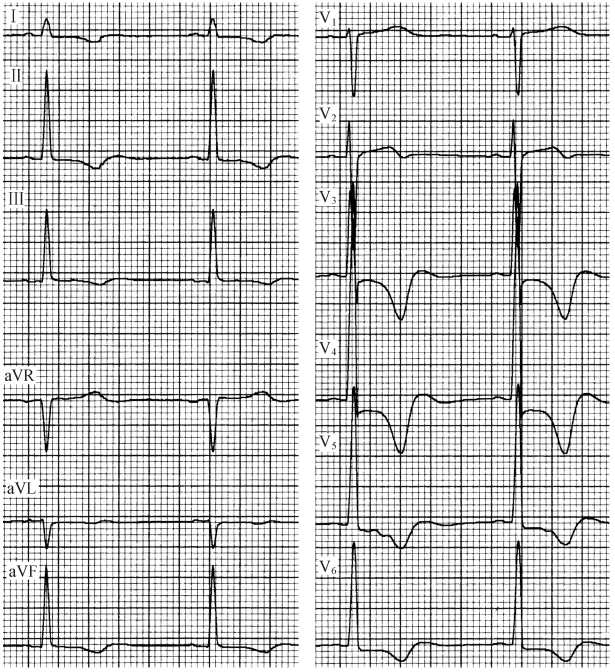
\includegraphics[width=4.15625in,height=4.54167in]{./images/Image00706.jpg}
 \captionsetup{justification=centering}
 \caption{男性,46岁,心尖部肥厚型心肌病(心尖厚度2.3cm),定准电压均为0.5mV。显示窦性心动过缓、左心室肥大伴劳损、前壁巨倒T波}
 \label{fig43-3}
  \end{figure} 

(1)持续性ST-T改变:最常见且最具特征性。ST段呈水平型或下斜型压低0.1~0.3mV,T波常呈对称性倒置,深度≥0.5~1.0mV,酷似“冠状T波”,以胸前导联尤其是V\textsubscript{3}
、V\textsubscript{4} 导联最为明显,多见于心尖部肥厚型心肌病。

(2)左心室高电压或左心室肥厚:R\textsubscript{V\textsubscript{5}}
及R\textsubscript{V\textsubscript{5}}
+S\textsubscript{V\textsubscript{1}}
电压均明显增高,有时V\textsubscript{1}
导联QRS波群呈Rs型,R波电压>1.0mV,这不是右心室肥大的表现,而是异常增厚的室间隔左侧面除极时所产生的向右前向量增大所致。

(3)窄而深的异常Q波:具有特征性改变,常见于Ⅱ、Ⅲ、aVF导联或V\textsubscript{5}
、V\textsubscript{6}
导联,同时这些导联R波电压增高,T波常直立,而有别于心肌梗死的异常Q波,多见于室间隔肥厚型心肌病。

(4)心电轴左偏。

(5)P波时间增宽:P波时间增宽与左心房肥大、左心房内传导障碍有关,因左心室顺应性降低,左心室舒张期末压增高,导致左心房负荷过重,久之将引起左心房肥大和左心房内传导障碍。

(6)心律失常:可见房性心律失常(房性早搏、房性心动过速、心房颤动)、传导阻滞(房室传导阻滞、束支阻滞)及室性心律失常(多源、多形性室性早搏、短阵性室性心动过速),以室性心律失常多见且易引发恶性心律失常而猝死。

(7)部分患者可出现预激综合征的图形。

5.诊断线索

(1)年轻男性患者,无高血压病史,出现左胸导联R波电压增高伴ST段压低、胸前导联T波倒置,应高度怀疑心尖部肥厚型心肌病。

(2)年轻男性患者,无高血压病史,出现左胸导联窄而深的异常Q波伴R波电压增高,T波直立,应高度怀疑室间隔肥厚型心肌病。

\protect\hypertarget{text00051.htmlux5cux23subid617}{}{}

\subsection{致心律失常性右室心肌病}

1.基本概念

致心律失常性右室心肌病是指右室心肌被脂肪浸润及纤维组织所替代,导致右心室弥漫性扩张、心室壁变薄变形、心肌萎缩、收缩运动进行性减弱,出现右室心力衰竭、右室源性心律失常及发作性晕厥为特征的原因不明的心肌病。主要见于青少年,约30\%有家族史,为常染色体显性遗传,是年轻人猝死的常见原因之一。

2.病理生理改变

右室心肌被脂肪浸润及纤维组织所替代,导致右心室扩张、收缩性减弱及右室心力衰竭,出现右心房负荷过重、扩大;病变累及传导组织,出现右心室内传导障碍及室性心律失常。

3.心电图特征

(1)P波高尖:系右心房负荷过重、肥大或扩张所致。

(2)局限性QRS波群时间增宽:右心室部分心肌除极延迟,导致局限性V\textsubscript{1}
~V\textsubscript{3}
导联QRS波群时间≥0.11s,其特异性为100\%,敏感性为55\%;如(V\textsubscript{1}
+V\textsubscript{2} +V\textsubscript{3}
)QRS波群时限/(V\textsubscript{4} +V\textsubscript{5}
+V\textsubscript{6}
)QRS波群时间≥1.2,则特异性为100\%,敏感性为93\%,反映了右心室部分心肌除极延迟,同时V\textsubscript{1}
~V\textsubscript{3} 导联的Q-T间期相应延长。

(3)右束支阻滞图形:约33\%的患者出现不同程度右束支阻滞图形,但阻滞部位并非真正地发生在右束支主干,而是发生在右心室壁内的传导障碍。如在右束支传导阻滞基础上,V\textsubscript{1}
~V\textsubscript{3} 导联QRS波群时间比V\textsubscript{6}
导联延长0.05s以上,则具有非常诊断意义。

(4)Epsilon波:V\textsubscript{1} 、V\textsubscript{2}
导联QRS波群终末部或ST段起始处出现向上小棘波,偶呈凹缺状,约持续0.02s,有时出现在右胸V\textsubscript{3}
R、V\textsubscript{4}
R导联。放大定准电压(20mm/mV),加快纸速(50mm/s),可提高检出率,或者用双极胸前导联(将右上肢导联用吸球吸在胸骨柄处作为阴极,左上肢导联用吸球吸在剑突处作为阳极,左下肢导联用吸球吸在V\textsubscript{4}
导联位置作为阳极,选择在Ⅰ、Ⅱ、Ⅲ导联进行记录),可提高检出率2~3倍。Epsilon波是致心律失常性右室心肌病一个特异性较强的心电图指标,具有诊断价值,是右心室被脂肪组织包绕的岛样有活性心肌细胞延迟除极所致(图\ref{fig43-4}、图\ref{fig43-5})。

\begin{figure}[!htbp]
 \centering
 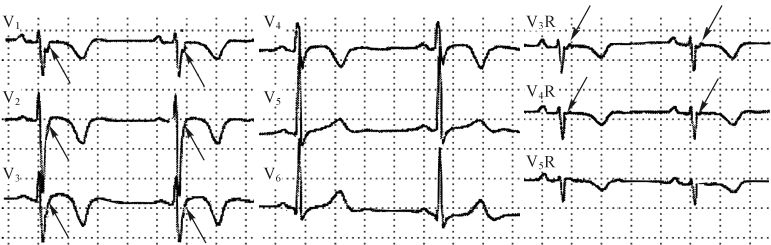
\includegraphics[width=5.20833in,height=1.65625in]{./images/Image00707.jpg}
 \captionsetup{justification=centering}
 \caption{女性,53岁,家族性致心律失常性右室心肌病。右胸导联出现Epsilon波及T波倒置(引自蔡海鹏)}
 \label{fig43-4}
  \end{figure} 

\begin{figure}[!htbp]
 \centering
 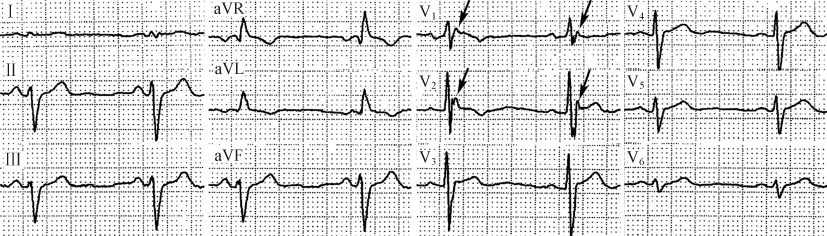
\includegraphics[width=5.58333in,height=1.59375in]{./images/Image00708.jpg}
 \captionsetup{justification=centering}
 \caption{男性,28岁,致心律失常性右室心肌病。显示V\textsubscript{1}导联有Epsilon波及间歇性T波倒置、QRS波群及部分T波电交替现象、假性电轴左偏-90°、顺钟向转位、右心室肥大?}
 \label{fig43-5}
  \end{figure} 
、V\textsubscript{2}


(5)心律失常:主要表现为起源于右心室的室性早搏和室性心动过速,其QRS波群呈类似左束支阻滞图形,其次为房性心律失常,如房性早搏、房性心动过速、心房扑动及颤动等。

(6)胸前导联T波倒置:为该心肌病的特征性表现之一,绝大多数发生在V\textsubscript{1}
~V\textsubscript{3} 导联,偶尔发生在V\textsubscript{1}
~V\textsubscript{6} 导联。

(7)心室晚电位阳性。

4.心电图诊断标准

Fisher提出致心律失常性右室心肌病的心电图诊断标准为:①V\textsubscript{1}
~V\textsubscript{3} 导联T波倒置;②出现V\textsubscript{1}
~V\textsubscript{3}
导联局限性QRS波群时限≥0.11s;③Epsilon波;④频发类似左束支阻滞型的室性早搏(>1000次/24h);⑤反复出现类似左束支阻滞型的室性心动过速;⑥心室晚电位阳性。

\protect\hypertarget{text00051.htmlux5cux23subid618}{}{}

\subsection{缺血性心肌病}

1.基本概念

缺血性心肌病是指由冠心病或冠状动脉末梢弥漫性病变引起心肌长期缺血缺氧,导致心肌纤维化,出现充血性心力衰竭为主的综合征,而不能用冠状动脉病变或缺血损伤程度来解释的收缩功能障碍。2006年美国心脏病协会建议不再使用“缺血性心肌病”这一命名。

2.病理生理改变

心脏肥大呈球形结构,心室壁厚薄交错不均匀,被大片疤痕组织代替,可累及右心室;心肌收缩力减退、心室顺应性降低,出现心力衰竭,并且反复发作。若累及传导组织,可出现各种心律失常及传导阻滞。

3.心电图改变

(1)异常Q波:反映心肌坏死、纤维化。

(2)缺血性ST-T改变。

(3)左心室高电压:V\textsubscript{5} 、V\textsubscript{6}
导联R波电压增高。

(4)Q-T间期延长。

(5)心律失常:以窦性心动过速、房性心律失常、室性心律失常等多见。

(6)传导阻滞:房室传导阻滞、束支阻滞、不定型心室内传导阻滞等。

4.诊断

诊断缺血性心肌病,必须具备3个肯定条件和2个否定条件。

(1)3个肯定条件为:①有明确的冠心病史,至少有≥1次心肌梗死或冠状动脉造影阳性;②心脏明显扩大;③顽固性心力衰竭。

(2)2个否定条件为:①排除冠心病并发症引起的室壁瘤、室间隔穿孔、乳头肌功能不全;②排除其他心脏病和其他原因引起的心脏扩大和心力衰竭。

\protect\hypertarget{text00051.htmlux5cux23subid619}{}{}

\subsection{围生期心肌病}

1.基本概念

围生期心肌病是指在妊娠过程中,特别是在妊娠末3个月至产后6个月内首次发生的以累及心肌为主的一种与妊娠有密切关系的心肌病。多发生在产后,以急性心力衰竭起病。

2.病理生理改变

与扩张型心肌病病理生理改变类似,4个心腔均有不同程度的扩张,但以左心室扩张最为显著。若病变累及传导系统,可出现各种心律失常和传导阻滞。

3.心电图改变

与扩张型心肌病心电图改变类似,主要表现为室性和房性心律失常、传导阻滞、非特异性STT改变及心房、心室扩大的心电图改变。

4.诊断

在确定围生期心肌病诊断之前,必须明确心力衰竭的原因,排除其他心脏病。Silber提出3条诊断标准:①既往无任何心脏病证据;②妊娠末3个月至产后6个月内出现心脏病及心力衰竭;③心脏病和心力衰竭不能用其他病因来解释。

\protect\hypertarget{text00051.htmlux5cux23subid620}{}{}

\subsection{心动过速性心肌病}

1.基本概念

各种长期反复发作的心动过速引起心脏进行性扩大、心功能减退,经积极治疗控制心动过速后,扩大的心脏会逐渐缩小,心功能部分或完全恢复正常,这种继发于心动过速性心肌疾病,称为心动过速性心肌病。

2.病因

心动过速是引起心肌病的直接原因。心动过速可分为阵发性室上性心动过速、心房扑动、心房颤动、室性心动过速、起搏器介导性心动过速及不适当性窦性心动过速等。心动过速持续时间越长,频率越快,则心肌受损越严重,病变越广泛。心动过速性心肌病的形成需要数年或更长时间。

3.分型

(1)单纯型:心动过速是导致心脏扩大、心功能异常的唯一因素,心脏无其他异常改变。

(2)混合型:除了心动过速外,尚合并其他导致心功能异常的病因。

4.病理生理改变

持续性心动过速或心动过速每天发作总时间超过10\%~15\%,将会导致心脏扩大,尤其是心室腔扩张,心室壁变薄,心脏收缩功能、舒张功能均减退,出现心力衰竭;若病变累及传导系统,还可出现各种心律失常和传导阻滞。

5.心电图改变

在原有心动过速基础上,可出现其他心律失常,如早搏、传导阻滞及非特异性ST-T改变等。

6.诊断

病史和临床表现是目前诊断心动过速性心肌病的唯一可靠手段,有心脏扩大或心力衰竭和持续性心动过速或反复发作心动过速的患者应高度怀疑此病。其诊断要点为:①心动过速发作前心功能正常;②在频繁发作或持续性心动过速后出现心功能进行性损害,并能排除其他因素影响;③心动过速治愈或控制后,扩大的心脏改善或恢复正常。

\protect\hypertarget{text00051.htmlux5cux23subid621}{}{}

\subsection{应激性心肌病}

1.基本概念

应激性心肌病由精神刺激所引发的左心室功能不全、影像学与心电图呈一过性改变的一组症候群。表现为:①发病初期患者胸痛,左心室造影及心脏超声心动图均有左心室心尖和前壁下段运动减弱或消失,基底部心肌运动代偿性增强;②左心室平均射血分数降低;③冠状动脉造影正常。

2.发病机制

与体内过高的儿茶酚胺对心肌细胞的直接毒性作用引起的心肌顿抑有关。

3.心电图改变

(1)类似急性心肌梗死,一般出现在发病后4~24h。

(2)发病急性期,绝大多数患者胸前导联出现ST段抬高(0.2~0.6mV)。

(3)半数患者在急性期和亚急性期(2~18d)T波逐渐转为倒置,T波出现深倒置是患者处于恢复期的心电图特征性表现。

(4)约1/3患者出现病理性Q波,常见于V\textsubscript{1}
~V\textsubscript{4} 导联。

(5)Q-T间期延长出现在发病后48h内,但很快恢复正常。

(6)可出现各种心律失常。

4.诊断依据

(1)发病年龄与性别:多发生于老年绝经期后的女性,女性发病率是男性的7倍。

(2)病史:发病前有强烈的心理或躯体应激状态。

(3)症状:绝大多数患者出现类似急性心肌梗死胸痛和呼吸困难。

(4)辅助检查:①心电图异常;②左心室造影及心脏超声心动图均提示一过性心室壁运动异常,左心室心尖和前壁下段运动减弱或消失,基底部心肌运动代偿性增强;③左心室平均射血分数降低;④冠状动脉造影正常;⑤心肌酶谱正常或轻度增高。

(5)转归:心功能常在短时间内恢复正常,预后一般良好。

\protect\hypertarget{text00052.html}{}{}

\protect\hypertarget{text00052.htmlux5cux23chapter52}{}{}

\chapter{经典的心肌梗死及其进展}

\protect\hypertarget{text00052.htmlux5cux23subid622}{}{}

\subsection{心脏的血液供应}

1.心肌的血液供应

左冠状动脉(左心室80\%的血液由其供应):起源于主动脉根部的左后主动脉窦,长约0.5~1.0cm,很快分为前降支、回旋支(左旋支),少数人还有对角支。

(1)前降支(左心室50\%的血液由其供应):①左心室前支,供应左心室前壁、前乳头肌;②右心室前支,供应右心室前壁;③前室间隔支(又称为前穿支),供应室间隔前上2/3部分、希氏束、左右束支及左前分支、左中隔支等。

(2)回旋支(左旋支):①左心室前支,供应左心室前壁;②左心室后支,供应左心室侧壁、后壁、后乳头肌;③左心房支,供应左心房;④左缘支,供应左心室的最外侧缘。

(3)对角支:供应左心室前壁的上部。

右冠状动脉(左心室20\%的血液由其供应):起源于右主动脉窦,在房室交接处作“U”字形弯曲,称为U袢,并延伸为后降支,分为右心房支、右心室支、后降支等。

(1)右心房支:供应右心房。

(2)右心室支:供应右心室前壁、侧壁。

(3)后降支:发出后室间隔支、右缘支,供应室间隔后下1/3部分、下壁、后壁、左后分支、窦房结、房室结等。

2.传导系统的血液供应

(1)窦房结:绝大多数由单支血管供应,即由窦房结动脉供血,约2/3发自右冠状动脉的近端,1/3发自左冠状动脉回旋支近端。窦房结动脉亦供应心房肌、房间隔的大部分及心房内传导组织。

(2)房室结:由多支血管供血,血源丰富,主要由房室结动脉供血,绝大部分起源于右冠状动脉远端的U袢,少部分发自左冠状动脉的回旋支;此外,房室结尚接受回旋支等动脉的血供。

(3)希氏束、束支:由房室结动脉、前室间隔支双重血管供应。急性心肌梗死时如发生左束支阻滞,提示左、右冠状动脉均有病变。

(4)分支:左前分支、左中隔支由前室间隔支供应,若前室间隔支发生阻塞,则可引起左前分支、左中隔支阻滞;左后分支由前室间隔支、后降支双重供血,故单纯性左后分支阻滞或右束支合并左后分支阻滞少见。

\protect\hypertarget{text00052.htmlux5cux23subid623}{}{}

\subsection{定位诊断与相关动脉病变部位的判断}

根据心电图相关导联出现的异常Q波、ST段改变、T波改变及传导阻滞类型,来推测可能是哪一支相关动脉发生病变。

(1)高侧壁心肌梗死及其相关病变的动脉:Ⅰ、aVL导联面对左心室高侧壁,该部位由回旋支的左缘支、左心室后支供血。若高侧壁发生心肌梗死,则其病变动脉为回旋支的左缘支、左心室后支部位。

(2)下壁心肌梗死及其病变的动脉:Ⅱ、Ⅲ、aVF导联面对左心室下壁,该部位多数患者由右冠状动脉的后降支和左心室后支供血(右冠状动脉优势)。若出现下壁、右心室心肌同时梗死,则其病变动脉为右冠状动脉近端、锐缘支发出前的部位(图\ref{fig44-1}A的A点);若仅为单纯的下壁心肌梗死,则为右冠状动脉锐缘支的远端(图\ref{fig44-1}A的B点)。而对左冠状动脉优势型患者,该部位由回旋支的左心室后支供血,若同时并发侧壁、正后壁、下壁心肌梗死,则其病变动脉为回旋支近端部位(图\ref{fig44-1}B的A点);若为单纯的下壁心肌梗死,则其病变动脉为左心室后支(图\ref{fig44-1}B的B点)。下壁心肌梗死易并发房室传导阻滞,且提示阻塞部位在U袢之前。

\begin{figure}[!htbp]
 \centering
 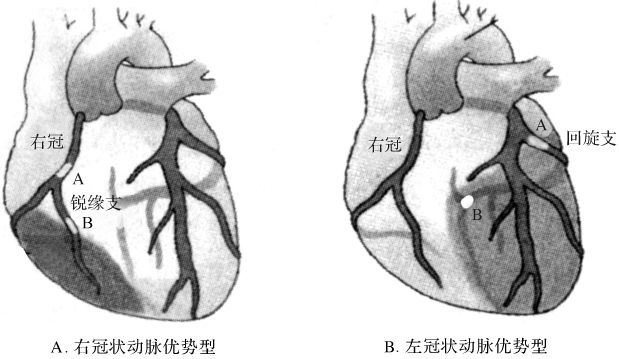
\includegraphics[width=4.17708in,height=2.42708in]{./images/Image00709.jpg}
 \captionsetup{justification=centering}
 \caption{下壁心肌梗死相关的病变动脉}
 \label{fig44-1}
  \end{figure} 

(3)前间壁心肌梗死及其病变的动脉:V\textsubscript{1}
、V\textsubscript{2} 、(V\textsubscript{3}
)导联面对左心室间隔的前部,该部位还含有希氏束、束支,由前室间隔支供血。若梗死部位局限在前间壁,则为间隔支近端发生阻塞(图\ref{fig44-2}的A点),且常合并右束支阻滞;若同时累及左心室前壁,则病变的动脉是前降支的间隔支发出之前(图\ref{fig44-2}的B点)。

\begin{figure}[!htbp]
 \centering
 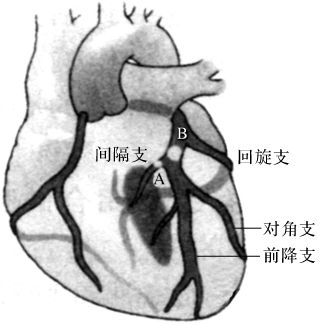
\includegraphics[width=2.15625in,height=2.19792in]{./images/Image00710.jpg}
 \captionsetup{justification=centering}
 \caption{前间壁心肌梗死相关的病变动脉}
 \label{fig44-2}
  \end{figure} 

(4)前壁心肌梗死及其病变的动脉:V\textsubscript{3} 、V\textsubscript{4}
、(V\textsubscript{5}
)导联面对左心室前壁,该部位由左前降支供血。若心肌梗死仅局限在V\textsubscript{3}
、V\textsubscript{4} 、(V\textsubscript{5}
)导联部位,则其病变动脉为左前降支中段(图\ref{fig44-3}的A点);若扩展到V\textsubscript{1}
、V\textsubscript{2} 导联,即V\textsubscript{1} ~V\textsubscript{5}
导联,则其病变动脉为左前降支近端(图\ref{fig44-3}的C点),易发生双束支阻滞或完全性房室传导阻滞。

\begin{figure}[!htbp]
 \centering
 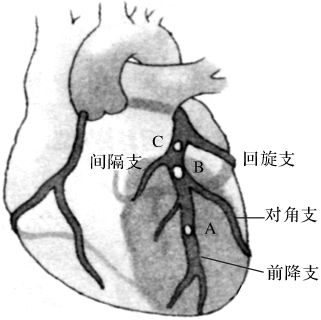
\includegraphics[width=2.16667in,height=2.15625in]{./images/Image00711.jpg}
 \captionsetup{justification=centering}
 \caption{前壁心肌梗死相关的病变动脉}
 \label{fig44-3}
  \end{figure} 

(5)前侧壁心肌梗死及其病变的动脉:V\textsubscript{4}
、V\textsubscript{5} 、V\textsubscript{6}
导联面对左心室前侧壁,该部位由左前降支供血。若前侧壁发生心肌梗死,则其病变动脉为左前降支发出对角支之前的B点部位(图\ref{fig44-3}的B点)。

(6)侧壁心肌梗死及其相关病变的动脉:Ⅰ、aVL、(V\textsubscript{5}
)和V\textsubscript{6}
导联面对左心室侧壁,该部位由回旋支、前降支和右冠状动脉右心室支供血。若侧壁发生心肌梗死,则其病变动脉为回旋支近端或对角支及前降支的近端部位(图\ref{fig44-4}的A、B点)。

\begin{figure}[!htbp]
 \centering
 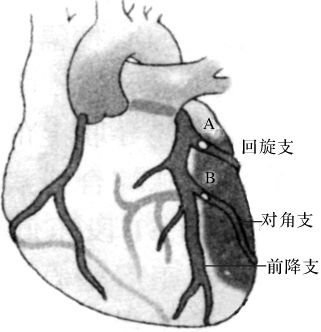
\includegraphics[width=2.16667in,height=2.23958in]{./images/Image00712.jpg}
 \captionsetup{justification=centering}
 \caption{侧壁心肌梗死相关的病变动脉}
 \label{fig44-4}
  \end{figure} 

(7)正后壁心肌梗死及其病变的动脉:V\textsubscript{7}
、V\textsubscript{8} 、(V\textsubscript{9}
)导联面对左心室正后壁,该部位多数患者由回旋支的左心室后支供血,少数由右冠状动脉后降支供血或由这两者共同供血。右冠状动脉优势患者,若同时并发下壁、正后壁心肌梗死,则其病变动脉为右冠状动脉近端;左冠状动脉优势型患者,若仅出现正后壁心肌梗死,则其病变动脉为钝缘支(图\ref{fig44-5})。

\begin{figure}[!htbp]
 \centering
 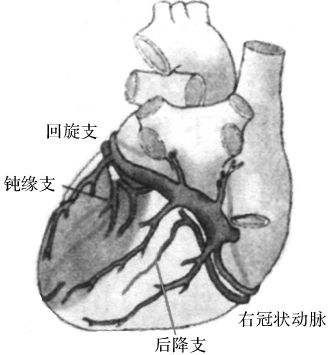
\includegraphics[width=2.21875in,height=2.39583in]{./images/Image00713.jpg}
 \captionsetup{justification=centering}
 \caption{正后壁心肌梗死相关的病变动脉}
 \label{fig44-5}
  \end{figure} 

(8)广泛前壁心肌梗死及其病变的动脉:Ⅰ、aVL、V\textsubscript{1}
~V\textsubscript{6}
导联面对左心室高侧壁、前间壁、前侧壁,称为广泛前壁。该部位由左冠状动脉前降支、回旋支及右冠状动脉后降支供血。若发生广泛前壁心肌梗死,表明上述冠状动脉发生病变,并且易出现双束支阻滞或完全性房室传导阻滞。

(9)右心室心肌梗死及其病变的动脉:需要加做右胸V\textsubscript{3}
R、V\textsubscript{4} R、V\textsubscript{5} R、V\textsubscript{6}
R导联,该部位由右冠状动脉的右心室支、左冠状动脉的前降支的右心室前支供血。单纯性右心室梗死少见,由右冠状动脉的锐缘支起始部阻塞所致(图\ref{fig44-6}的B点);右心室梗死往往伴发下壁梗死,由右冠状动脉近端、锐缘支发出前的部位发生阻塞所致(图\ref{fig44-6}的A点)。故下壁心肌梗死时,一定要注意是否同时伴发了右心室梗死,应当加做右胸导联。

\begin{figure}[!htbp]
 \centering
 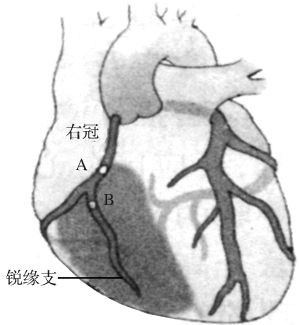
\includegraphics[width=2.02083in,height=2.19792in]{./images/Image00714.jpg}
 \captionsetup{justification=centering}
 \caption{右心室心肌梗死相关的病变动脉}
 \label{fig44-6}
  \end{figure} 

(10)心房梗死及其病变的动脉:心房的血液由回旋支的左心房支和右冠状动脉的右心房支供应。单纯性心房梗死少见,并且易并发房性心律失常。

\protect\hypertarget{text00052.htmlux5cux23subid624}{}{}

\subsection{心肌梗死的基本心电图改变}

冠状动脉粥样硬化引起管腔狭窄、斑块脱落、血栓形成而导致某一支冠状动脉突然阻塞或冠状动脉发生严重而持久痉挛性闭塞引起心肌急性缺血、损伤直至坏死,产生一系列特征性的心电图改变:中心区表现为坏死型异常Q波,中间区表现为损伤型ST段抬高,外侧区表现为缺血型T波倒置。

(一)缺血型T波改变

缺血型T波改变是冠状动脉急性闭塞后最早出现的改变,首先表现为T波直立高耸,两肢基本对称,呈帐篷状,振幅可高达2.0mV,对早期诊断急性心肌梗死具有重要的临床意义。数分钟至数小时后,T波很快由高耸转为倒置。

(1)心内膜下心肌缺血:通常缺血最早发生在心内膜下心肌层,面对缺血区导联出现T波直立高耸,两肢基本对称,基底部变窄,呈帐篷状,类似高钾血症的T波改变。

(2)心外膜下心肌缺血:随着缺血的进一步加重,出现心外膜下心肌缺血,面对缺血区导联的T波两肢呈对称性倒置,表现为冠状T波。

(3)穿壁性心肌缺血:倒置的T波进一步加深,伴Q-T间期延长。

(二)损伤型ST段改变

随着心肌缺血进一步加重,将出现损伤型ST段改变,表现为面对损伤区导联出现ST段抬高或压低,为急性心肌梗死早期的另一种心电图表现。ST段抬高的形态、程度及其动态演变对诊断急性心肌梗死和预后判断都具有重要的临床意义。

(1)心内膜下心肌损伤:面对损伤区导联出现ST段呈水平型、下斜型压低≥0.1mV。

(2)心外膜下心肌损伤:面对损伤区导联ST段呈斜直型、弓背向上型、单相曲线型、墓碑型、巨R型抬高≥0.1mV。

(3)穿壁性心肌损伤:ST段抬高更加明显,多>0.5mV。

(三)坏死型QRS波群改变

持续而严重的心肌缺血、损伤,将导致心肌坏死,出现异常Q波,包括组织学上的坏死和电学上的“电静止”,后者是由于心肌细胞膜电位负值降至阈电位以下,暂时丧失了电活动能力,即出现心肌顿抑现象,供血改善后,异常Q波可消失。多数患者在急性心肌梗死发生后6~14h出现异常Q波。

1.异常Q波(病理性Q波)的诊断标准

(1)旧标准:①Q波时间≥0.04s;②Q波深度≥$\frac{1}{4}$
R;③呈QS型,起始部错折;④出现胚胎型r波,即呈qrS型或QrS型。

(2)新标准:相邻两个导联的Q波时间≥0.03s、深度≥0.1mV,但不包括Ⅲ、aVR导联。

2.异常Q波形成的条件

(1)心肌梗死范围:梗死区直径>2.0~3.0cm时,将产生异常Q波。若梗死区直径<2.0cm,累及左心室≤10\%,则不会出现异常Q波,仅出现q波或等位性Q波。

(2)心肌梗死深度:梗死厚度>0.5~0.7cm,累及左心室厚度的50\%以上时,将产生异常Q波。人的心内膜厚度约占心室壁的50\%,若梗死厚度<50\%,则不会出现异常Q波,仅引起QRS波形改变,如顿挫、切迹、R波电压降低等。

(3)心肌梗死部位:出现异常Q波,除了心肌梗死范围足够大、深度足够深外,梗死区还必须是在QRS起始0.04s部位。否则,不会出现异常Q波,如基底部梗死,仅引起QRS终末0.04s处切迹、顿挫或S波加深。

3.等位性Q波(或相当性Q波)

等位性Q波是指因梗死面积较少或局限于基底部、心尖部或梗死极早期尚未充分发展等原因,未形成典型的异常Q波,仅产生各种特征性QRS波形改变,这些伴随临床症状出现的特征性QRS波形改变与异常Q波有等同的诊断价值,称为等位性Q波或相当性Q波,但必须结合临床及同导联ST-T改变情况。

(1)部分q波:当梗死面积较小,虽位于QRS起始0.04s除极部位,但不能形成典型的异常Q波,仅出现q波:①V\textsubscript{1}
~V\textsubscript{6} 导联均出现q波;②V\textsubscript{3}
~V\textsubscript{6}
导联q波宽于和深于下一个胸前导联q波,即qV\textsubscript{3}
>qV\textsubscript{4} >qV\textsubscript{5} >qV\textsubscript{6}
;③右胸导联出现q波,而左胸导联q波消失,能排除右心室肥大、左前分支阻滞,即V\textsubscript{1}
、V\textsubscript{2} 导联出现q波而V\textsubscript{5}
、V\textsubscript{6}
导联未见q波;④下壁导联Ⅱ导联有q波,Ⅲ导联呈Q波,aVF导联q波时间0.03s左右,深度接近$\frac{1}{4}$
R。

(2)QRS波群起始部切迹、顿挫:V\textsubscript{4} ~V\textsubscript{6}
导联QRS起始部出现≥0.05mV负相波,即呈rsR′型,与心尖部心肌梗死或前壁小面积心肌梗死有关。

(3)进展性Q波:同一患者在相同体位、部位进行动态观察,原有q波进行性增宽、加深,或原无q波的导联出现新的q波。

(4)存在病理性Q波区:某个胸前导联q波虽未达到病理性Q波的诊断标准,但在其导联周围(上、下或左、右)均可记录到Q波,表明存在病理性Q波区域,为诊断心肌梗死有力佐证。

(5)R波电压变化:①动态观察,同一导联R波电压进行性降低,又称为R波丢失;②胸前导联R波振幅逆递增,如rV\textsubscript{2}
>rV\textsubscript{3} >rV\textsubscript{4}
;③胸前导联R波振幅递进不良,如V\textsubscript{1} ~V\textsubscript{4}
导联,r波振幅递进量<0.1mV;④右胸导联V\textsubscript{3}
R、V\textsubscript{1} 、V\textsubscript{2}
导联R波电压增高伴T波高耸,呈镜像改变,表明存在正后壁心肌梗死,应加做V\textsubscript{7}
、V\textsubscript{8} 、V\textsubscript{9}
导联;⑤Ⅱ导联有Q波,Ⅲ、aVF导联未见q波或Q波,但其QRS波群电压≤0.25mV,或Ⅱ导联R波电压≤0.25mV伴Ⅲ、aVF导联有Q波;⑥相邻的两个胸前导联的R波振幅相差≥50\%,如R\textsubscript{V\textsubscript{3}}
>$\frac{1}{2}$
R\textsubscript{V\textsubscript{4}}
;⑦新消失的室间隔q波,即Ⅰ、aVL、V\textsubscript{5} 、V\textsubscript{6}
导联q波消失或减小。

\protect\hypertarget{text00052.htmlux5cux23subid625}{}{}

\subsection{急性心肌梗死的诊断标准及心电图分类}

1.急性心肌梗死的诊断标准

临床对急性心肌梗死的诊断一直沿用WHO的诊断标准:①有缺血性胸痛症状;②有心电图特征性ST-T动态演变或伴异常Q波;③有血清心肌酶谱升高与回落。满足其中2条者,即可诊断。2000年,欧洲/美国心脏病学会重新修订了急性心肌梗死的诊断标准,即有典型心肌坏死生化标志物(肌钙蛋白或CK-MB)的升高与回落,同时伴有下列1项者,即可诊断为急性心肌梗死:①有心肌缺血症状;②出现病理性Q波;③有ST段抬高或压低;④冠状动脉介入治疗(PTCA)术后。

2.急性心肌梗死的心电图分类

急性心肌梗死的心电图分类经历了三个阶段:

(1)透壁性和非透壁性心肌梗死:20世纪80年代前沿用此分类方法,现已废弃不用。

(2)有Q波和非Q波心肌梗死:20世纪80年代后,根据有无出现Q波对心肌梗死进行分类。但出现Q波,意味着心肌细胞已坏死,不能满足临床早诊断、早干预、挽救濒死心肌的需求。但由于该分类方法简单明确,且两者在临床和预后上均有很大差异,故这一分类方法对临床仍有一定参考价值。无Q波心肌梗死者,其冠状动脉新形成的血栓较少、侧支循环较丰富、心肌损伤标志物水平较低,心肌灌注缺损不均匀较轻,心室壁运动异常程度较轻,心力衰竭发生率及近期死亡率均较低,但再梗死发生率高;而有Q波心肌梗死者,则刚好相反。

(3)ST段抬高型和非ST段抬高型梗死:近年来,国内外均采用ST段抬高型和非ST段抬高型进行分类,使心肌梗死诊断的时间大大提前,为早干预、早治疗、挽救濒死心肌赢得了宝贵时间,极大地改善了患者的预后,突出了早期干预的重要性和“时间就是心肌”的诊治理念。

ST段抬高型:相关导联先表现为T波高耸呈帐篷状,继之ST段呈斜直型、弓背向上型、单相曲线型,甚至墓碑型、巨R型抬高。ST段抬高是冠状动脉闭塞早期的心电图表现,是早期干预的标志。若心绞痛患者经治疗后不能缓解,持续时间达20min以上,相邻两个或两个以上导联ST段抬高(胸前导联抬高≥0.2mV、肢体导联抬高≥0.1mV),高度提示发生了急性心肌梗死,需尽早干预,挽救濒死心肌;否则,大部分患者将发展为Q波性心肌梗死。经治疗后,抬高的ST段快速回落(2h内回落>50\%)是冠状动脉再通的无创指标,少数患者可出现再灌注性损伤,表现为ST段快速回落前呈现一过性再抬高。

非ST段抬高型:大多数非Q波性心肌梗死,相关导联ST段呈水平型、下斜型压低≥0.2mV,持续时间>24h,或(和)伴有T波对称性倒置及其动态演变,诊断时,需结合临床症状及心肌损伤标志物升高(肌钙蛋白、CK-MB)。

\protect\hypertarget{text00052.htmlux5cux23subid626}{}{}

\subsection{心肌梗死的心电图演变规律及分期}

随着急性心肌梗死诊断新标准的实施,早诊断、早干预,实施早期再灌注治疗,挽救了许多濒死的心肌细胞,缩小了梗死范围,缩短了心肌梗死的病程,降低了异常Q波的发生率,部分地改变了心肌梗死心电图的演变规律。传统的心肌梗死心电图可分为超急性期、急性期、亚急性期(演变期)及陈旧期(慢性期)4期。亦有学者将其分为急性期、亚急性期及慢性期3期,其中急性期又分为3个亚期:超急性期(T波改变期)、进展期或急性早期(ST段改变期)、心肌梗死确定期(Q波及非Q波期)。

1.超急性期

超急性期又称为超急性损伤期,是急性心肌梗死最早期阶段,在冠状动脉闭塞后立即出现,持续时间极为短暂,约数分钟至数小时。心电图表现为相关导联T波高耸、ST段上斜型或斜直型抬高、急性损伤性阻滞及心律失常(图\ref{fig44-7})。

\begin{figure}[!htbp]
 \centering
 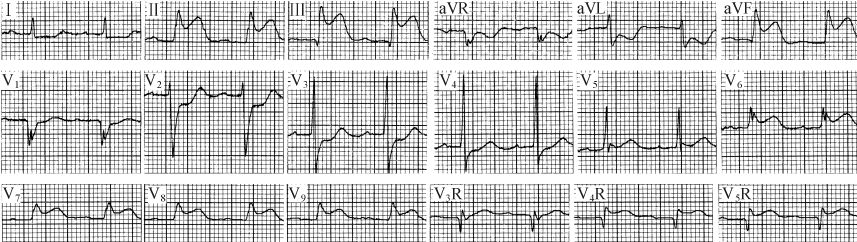
\includegraphics[width=5.79167in,height=1.63542in]{./images/Image00715.jpg}
 \captionsetup{justification=centering}
 \caption{男性,68岁,胸痛发作0.5h。显示下壁、后侧壁及右心室超急性期心肌梗死、前间壁ST段改变}
 \label{fig44-7}
  \end{figure} 

(1)T波高耸呈“帐篷状”改变:与细胞内K\textsubscript{+}
大量逸出而呈短暂性细胞外高\textsubscript{K}
+状态有关,如不及时干预治疗,异常Q波将出现在T波高耸的导联上。

(2)ST段呈上斜型或斜直型抬高:出现在T波高耸的导联上。

(3)急性损伤性阻滞:与损伤区域心肌组织传导延缓有关,表现为QRS波群轻度增宽(为0.11~0.12s)、振幅略增高。该现象持续时间较短,发生在异常Q波和T波倒置之前。

(4)U波倒置。

(5)出现各种室性心律失常:与损伤区域心肌处于严重的电生理紊乱状态有关。

2.急性期

从超急性期过度到急性期,在异常Q波尚未出现前,心电图可出现一过性假性正常化波形。急性期发生在梗死后数小时至数天内。

(1)出现异常Q波:梗死区相关导联出现异常Q波,与心肌细胞组织学上坏死或电学上坏死即“电静止”有关,后者经积极治疗后,异常Q波可消失。

(2)损伤型ST段抬高:可呈弓背向上型、单向曲线型、墓碑型、巨R型抬高(图\ref{fig44-8})。

\begin{figure}[!htbp]
 \centering
 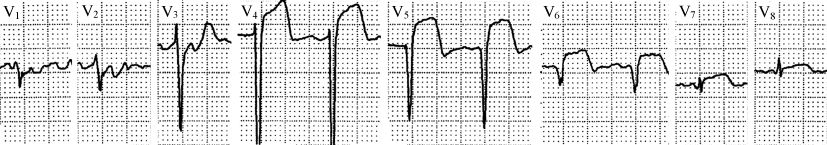
\includegraphics[width=5.58333in,height=0.97917in]{./images/Image00716.jpg}
 \captionsetup{justification=centering}
 \caption{男性,71岁,冠心病。显示心房颤动、前侧壁急性期心肌梗死}
 \label{fig44-8}
  \end{figure} 

(3)冠状T波:高耸的T波逐渐下降并呈对称性倒置

3.亚急性期(演变期)

持续时间约数周至数月。

(1)相对稳定的异常Q波或R波振幅降低。

(2)抬高的ST段逐渐回至基线或呈稳定性抬高(与室壁瘤形成有关)。

(3)T波动态演变:T波逐渐加深,又逐渐变浅转为低平或直立,也可呈恒定性T波倒置(图\ref{fig44-9})。

\begin{figure}[!htbp]
 \centering
 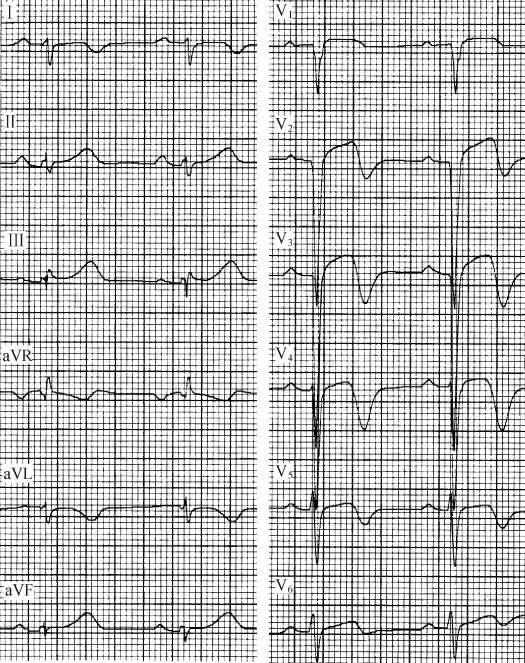
\includegraphics[width=3.54167in,height=4.47917in]{./images/Image00717.jpg}
 \captionsetup{justification=centering}
 \caption{男性,78岁,急性心肌梗死后1月余。显示肢体导联QRS波群低电压、前间壁异常Q波及前壁R波振幅降低伴T波改变(符合亚急性期心肌梗死)、高侧壁T波改变、Q-T间期延长}
 \label{fig44-9}
  \end{figure} 

4.陈旧性期(慢性稳定期)

临床上规定急性心肌梗死发病1个月后,即称为陈旧性期。一般情况以>3个月为陈旧性期。

(1)异常Q波很少有变化或转为QR、Qr型或转为q波或Q波消失。

(2)ST段恢复正常或呈缺血型压低或呈恒定性抬高。

(3)T波恢复正常或低平、倒置或呈恒定性冠状T波(图\ref{fig44-10}、图\ref{fig44-11})。

\begin{figure}[!htbp]
 \centering
 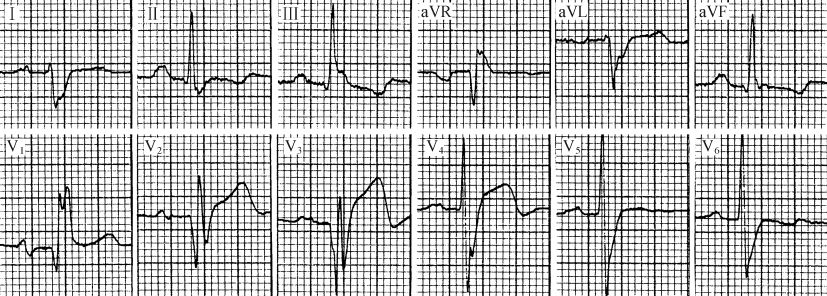
\includegraphics[width=5.58333in,height=2in]{./images/Image00718.jpg}
 \captionsetup{justification=centering}
 \caption{男性,64岁,陈旧性心肌梗死3年余。显示前间壁异常Q波(符合陈旧性期心肌梗死)、完全性右束支阻滞、左后分支阻滞、下壁及前侧壁T波改变}
 \label{fig44-10}
  \end{figure} 

\begin{figure}[!htbp]
 \centering
 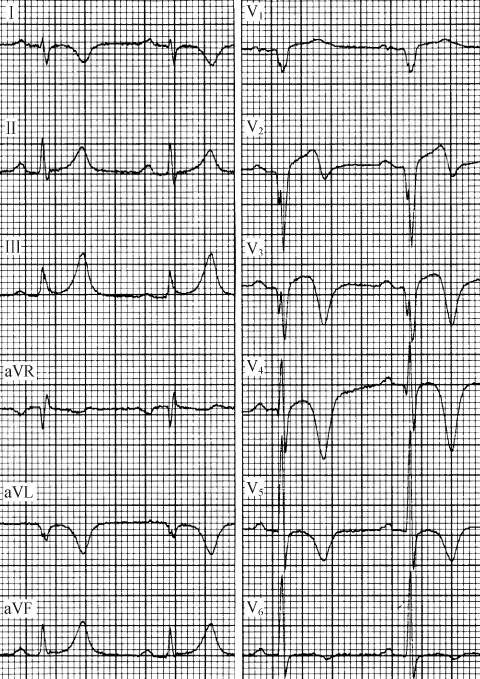
\includegraphics[width=3.23958in,height=4.58333in]{./images/Image00719.jpg}
 \captionsetup{justification=centering}
 \caption{男性,75岁,心肌梗死8个月。显示高侧壁、前间壁及局限性前壁异常Q波伴T波改变(符合陈旧性期心肌梗死)、前侧壁T波改变}
 \label{fig44-11}
  \end{figure} 

\protect\hypertarget{text00052.htmlux5cux23subid627}{}{}

\subsection{远离梗死区ST段改变的临床意义}

面对梗死区的导联出现异常Q波、损伤性ST段抬高、缺血性T波倒置,称为指示性改变。而与上述对应的导联出现R波振幅增高、ST段压低、T波高耸,则称为对应性改变,如下壁急性心肌梗死时,Ⅱ、Ⅲ、aVF导联ST段抬高,而Ⅰ、aVL导联ST段压低;后壁急性心肌梗死时,V\textsubscript{7}
、V\textsubscript{8} 、V\textsubscript{9}
导联出现异常Q波、ST段抬高、T波倒置,而V\textsubscript{3}
R、V\textsubscript{1} 、V\textsubscript{2}
导联出现R波增高、ST段压低、T波高耸。还有一部分远离梗死区的导联出现ST段压低者,则称为远离性ST段改变,其住院病死率和心肌梗死复发率均高于无ST段压低者,常合并多支血管病变,具有重要临床意义。

1.下壁急性心肌梗死伴其他导联ST段压低

(1)伴V\textsubscript{1} ~V\textsubscript{3}
导联ST段压低≥0.1mV(图\ref{fig44-7}):提示下壁梗死面积较大,多累及后侧壁、室间隔后下1/3部,由右冠状动脉近端阻塞所致,或者除了右冠状动脉阻塞(远端阻塞多见)外,尚合并回旋支阻塞(约占27\%)。若V\textsubscript{2}
导联ST段压低幅度与aVF导联ST段抬高幅度的比值≤0.5,则往往提示合并右心室急性心肌梗死;若V\textsubscript{3}
导联ST段压低幅度与Ⅲ导联ST段抬高幅度比值<0.5,则提示右冠状动脉近端阻塞;若比值在0.5~1.2之间,则提示右冠状动脉远端阻塞;若比值>1.2,则提示回旋支阻塞。

(2)伴V\textsubscript{4} ~V\textsubscript{5}
导联ST段压低≥0.1mV:比V\textsubscript{1} ~V\textsubscript{3}
导联ST段压低更具严重意义,其左心室功能更差、并发症更多,早期及远期(1~5年)死亡率明显高于无ST段压低者。多伴有前降支病变,且右冠状动脉近端阻塞及合并三支冠状动脉病变者明显高于无ST段压低者及V\textsubscript{1}
~V\textsubscript{3} 导联ST段压低者,侧支循环更差。

(3)伴侧壁(Ⅰ、aVL、V\textsubscript{6}
)导联ST段压低≥0.1mV:除了对应性改变外,还可能合并回旋支的左缘支病变。

(4)伴aVR导联ST段压低≥0.1mV:提示下壁梗死面积较大,心肌酶谱峰值较高,并发症发生率增高。

2.下壁急性心肌梗死伴其他导联ST段抬高

(1)伴V\textsubscript{1} ~V\textsubscript{3}
导联ST段抬高:为下壁梗死合并右心室梗死的象征。

(2)伴侧壁(Ⅰ、aVL、V\textsubscript{6}
)一个或数个导联ST段抬高:90\%由回旋支近端(钝缘支开口前)阻塞所致。

3.前壁急性心肌梗死伴其他导联ST段改变

前壁心肌梗死时,只要有任一导联ST段压低,其远期病死率高,此后发生心脏事件多。

(1)伴下壁导联ST段压低:前壁急性心肌梗死者伴下壁导联ST段压低,除了对应性改变外,还提示前壁心肌严重缺血及左前降支近端闭塞或远端闭塞合并第1对角支病变,为心肌梗死面积大、心功能差、并发症多、预后差的表现。

(2)伴aVR导联ST段抬高:提示左前降支阻塞位于左心室前支近端。

4.前侧壁急性心肌梗死伴aVR导联ST段压低

提示心肌梗死面积较大,心肌酶谱峰值较高,住院过程充血性心力衰竭发生率高,心功能较差,LVEF≤35\%。

\protect\hypertarget{text00052.htmlux5cux23subid628}{}{}

\subsection{特殊类型的心肌梗死}

1.右心室心肌梗死

单纯性右心室心肌梗死是罕见的,往往是下壁或下后壁急性心肌梗死波及右心室心肌而出现右心室心肌梗死。下壁、下后壁约40\%~50\%合并右心室梗死,均由右冠状动脉近端或右心室缘支近端阻塞所致。因此,对前间壁、下壁及后壁急性心肌梗死患者,必须加做V\textsubscript{3}
R、V\textsubscript{4} R、V\textsubscript{5} R、V\textsubscript{6}
R及V\textsubscript{7} 、V\textsubscript{8} 、V\textsubscript{9}
导联,以免漏诊。

(1)右心室心肌梗死的心电图改变:①V\textsubscript{3}
R~V\textsubscript{6}
R导联ST段抬高≥0.1mV,出现较早,且发病后24h内大多降至基线,以V\textsubscript{4}
R导联ST段抬高敏感性和特异性最高;②QRS波群在V\textsubscript{1}
导联呈rS型,在V\textsubscript{3} R~V\textsubscript{6}
R导联呈QS型;③V\textsubscript{1} ~V\textsubscript{3}
导联ST段呈损伤型抬高,但其抬高程度逐渐减轻且无异常Q波出现或V\textsubscript{1}
导联ST段抬高,V\textsubscript{2} 导联ST段压低。

(2)下壁急性心肌梗死时,出现下列改变者,强烈提示合并右心室梗死:①Ⅲ导联ST段抬高>Ⅱ导联ST段抬高,且ST\textsubscript{Ⅱ、Ⅲ}
≥0.1mV,诊断价值仅次于V\textsubscript{3} R~V\textsubscript{6}
R导联ST段抬高,诊断符合率达72\%~100\%(图\ref{fig44-7});②V\textsubscript{1}
~V\textsubscript{3}
导联ST段抬高,且抬高程度逐渐减轻或V\textsubscript{1}
导联ST段抬高≥0.1mV,而V\textsubscript{2}
导联ST段压低;③V\textsubscript{2}
导联ST段压低幅度与aVF导联ST段抬高幅度的比值≤0.5者,其敏感性为80\%左右,特异性90\%以上;④Ⅰ、aVL导联ST段压低>0.2mV者。

(3)正后壁急性梗死时,当V\textsubscript{1} ~V\textsubscript{3}
导联ST段压低不明显时,应高度怀疑合并右心室急性心肌梗死。

(4)下壁、正后壁急性心肌梗死合并电轴右偏、Ⅰ、aVL、V\textsubscript{5}
、V\textsubscript{6}
导联Q波消失,应高度怀疑合并右心室急性心肌梗死,因室间隔Q波消失与右冠状动脉病变引起右心室缺血具有高度相关性(图\ref{fig44-7})。

(5)在临床上,若遇及下壁、下后壁急性心肌梗死患者出现急性右心功能衰竭或窦性心动过缓、窦性停搏、房性心律失常(可能合并心房梗死)、房室传导阻滞、右束支阻滞等改变时,亦应高度怀疑合并右心室急性心肌梗死。

2.心内膜下心肌梗死

急性心内膜下心肌梗死有超急性期和急性期两个时相,心电图主要表现为ST-T的动态演变。

(1)面对梗死区导联ST段呈缺血型显著而持久地压低(图\ref{fig44-12}):以V\textsubscript{2}
~V\textsubscript{5}
导联最多见,ST段压低≥0.1mV,发病后第2~4天ST段压低达最大值,以后逐渐恢复正常。

\begin{figure}[!htbp]
 \centering
 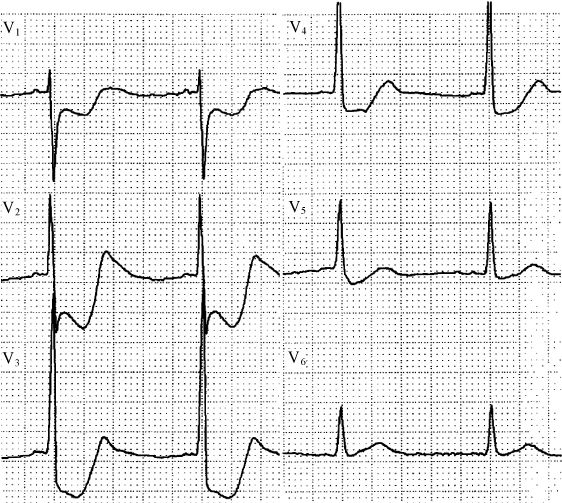
\includegraphics[width=3.79167in,height=3.39583in]{./images/Image00720.jpg}
 \captionsetup{justification=centering}
 \caption{前间壁、局限性前壁急性心内膜下心肌梗死}
 \label{fig44-12}
  \end{figure} 

(2)面对梗死区导联T波倒置呈“冠状T波”(图\ref{fig6-3}):ST段压低的导联,其T波倒置逐渐加深,呈“冠状T波”,约持续1周后,T波又逐渐变浅或转为正常。

(3)不出现异常Q波,面对梗死区导联的R波振幅降低或进行性降低。

(4)Q-T间期延长。

在临床上,若遇胸痛患者经治疗后,胸痛持续时间超过20min而不能缓解,出现上述心电图改变伴心肌坏死生化标志物增高,可诊断为急性心内膜下心肌梗死。

3.再发性心肌梗死(复发性心肌梗死)

(1)基本概念:在原有心肌梗死基础上再次发生新的心肌梗死,称为再发性心肌梗死。包括原心肌梗死灶延伸、毗邻原梗死区或远离原梗死区的部位发生新的梗死灶这3种类型。

(2)类型及其心电图特征

原梗死灶延伸:是指急性心肌梗死后4周内(以2周内多见),同一支血管供血区域的心肌再次发生梗死,使原梗死灶范围或深度扩大,导致原为非穿壁性或心内膜下梗死延伸为穿壁性心肌梗死,出现Q波型心肌梗死,或者延伸至梗死区毗邻部位使其发生急性心肌梗死。心电图特征:①坏死性Q波增深增宽,或由q波转为Q波或QS波,或QRS波幅降低;②ST段再度抬高,且ST-T呈动态演变(图\ref{fig44-13});③毗邻原梗死区的导联亦出现ST段抬高、ST-T动态演变,可伴有异常Q波出现。

\begin{figure}[!htbp]
 \centering
 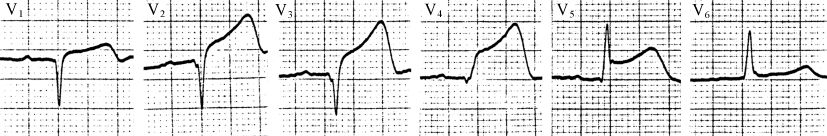
\includegraphics[width=5.58333in,height=0.91667in]{./images/Image00721.jpg}
 \captionsetup{justification=centering}
 \caption{男性,72岁,陈旧性心肌梗死1年余、再发胸痛0.5h。显示一度房室传导阻滞、前间壁及局限性前壁异常Q波、前间壁及前壁ST-T改变(提示又发生超急性期心肌梗死)、Q-T间期延长}
 \label{fig44-13}
  \end{figure} 

远离梗死区部位再梗死:是指首次心肌梗死后,再过若干时间,其他部位又发生新的急性心肌梗死。心电图特征:①原陈旧性梗死图形与新发生的急性心肌梗死图形并存。②当新发的梗死部位与原陈旧性梗死部位相对应时,若梗死范围大致相等,则表现为原有异常Q波消失,仅出现新发梗死区域导联ST段抬高及T波改变;若新发的梗死面积较大,则显示新发的梗死图形,而原有的梗死图形可部分或全部被掩盖。

(3)提高对再发性心肌梗死的警惕性:原发生过心肌梗死患者,若又出现不能缓解的胸痛或不明原因的心力衰竭、心源性休克,应高度警惕再发性心肌梗死的可能,特别注意以下心电图改变:①新出现q波或Q波伴ST段抬高;②QRS波群电压降低、切迹较多、时间增宽;③原有Q波增深、增宽或由q波转为Q波、QS波;④原有ST-T改变突然发生改变,甚至出现伪善性“正常”图形;⑤心电轴改变;⑥新出现房室传导阻滞、束支阻滞、室性心律失常或V\textsubscript{1}
Ptf增大。

4.心房梗死

单纯性心房梗死极其罕见,绝大部分是伴随着左心室梗死,右心房梗死比左心房梗死多见。心电图上可表现为PR段抬高或压低、P波呈M型或W型、房性心律失常、房室传导阻滞及窦性心动过速或过缓、停搏等。

5.从室性异位搏动图形中诊断心肌梗死

极少数急性心肌梗死患者,基本QRS-T波形正常,无异常Q波、ST段损伤型抬高和T波倒置,但在室性早搏QRS波群中却呈QR、QRs、qR型,ST段呈损伤型抬高伴T波高尖或倒置,显现急性心肌梗死的图形特征。可能由于基本节律引起室间隔前下1/3左心室面除极与左心室游离壁除极时,其向量指向了左前方,使心肌梗死的波形特征被掩盖。当出现室性早搏引起心室非同步除极时,梗死图形才在室性早搏中充分显示出来。从室性早搏QRS波形中诊断心肌梗死必须符合以下先决条件:①室性早搏QRS主波必须向上;②必须是反映心室电势的左胸导联(图\ref{fig44-14})。

\begin{figure}[!htbp]
 \centering
 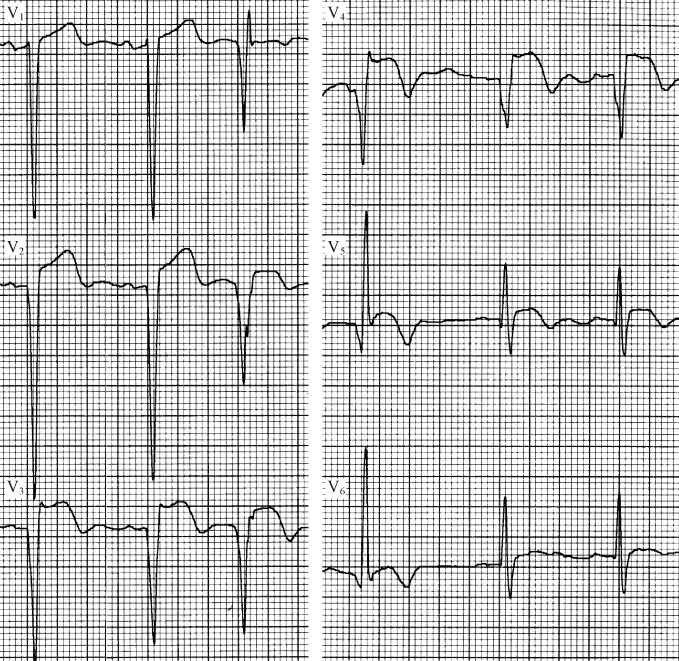
\includegraphics[width=4.58333in,height=4.46875in]{./images/Image00722.jpg}
 \captionsetup{justification=centering}
 \caption{前间壁、前壁异常Q波伴ST-T改变,符合急性心肌梗死;室性早搏的QRS-T波群亦显示急性心肌梗死波形特征(V\textsubscript{1}~V\textsubscript{3} 导联第3个搏动、V\textsubscript{4}~V\textsubscript{6} 导联第1个搏动)}
 \label{fig44-14}
  \end{figure} 


\protect\hypertarget{text00052.htmlux5cux23subid629}{}{}

\subsection{心肌梗死合并心室除极异常时的诊断}

凡是能影响QRS初始向量的心室除极异常,均能掩盖心肌梗死的典型图形,给诊断带来困难,如左束支阻滞、左前分支阻滞、预激综合征、室性异位心律、心室人工起搏心律等。

1.心肌梗死合并左束支阻滞

发生率约为8\%,心室初始除极向量发生了改变(室间隔除极从右下向左上进行),左心室延迟缓慢除极,心肌梗死典型图形将被掩盖。此时,ST-T改变和动态演变、左束支阻滞QRS波形不典型的改变为心肌梗死的诊断提供线索和佐证,ST段抬高导联即是梗死灶的部位。有以下心电图表现者,可提示左束支阻滞合并心肌梗死:

(1)与QRS主波同向的导联,其ST段抬高≥0.1mV,即以R波为主导联ST段抬高≥0.1mV,如V\textsubscript{5}
、V\textsubscript{6} 导联ST段抬高≥0.1mV。

(2)与QRS主波异向的导联,其ST段抬高≥0.5mV,即以S波为主导联ST段抬高≥0.5mV,如V\textsubscript{1}
、V\textsubscript{2} 导联ST段抬高≥0.5mV。

(3)与QRS主波异向的导联,其ST段压低≥0.1mV,即以S波为主导联ST段压低≥0.1mV,如V\textsubscript{1}
~V\textsubscript{3} 导联ST段压低≥0.1mV。

(4)若V\textsubscript{1}
导联QRS波群初始r波振幅增高,Ⅰ、aVL、V\textsubscript{5}
、V\textsubscript{6}
导联出现q波,则提示合并右下室间隔梗死;如伴rV\textsubscript{1}
>rV\textsubscript{2} >rV\textsubscript{3} 及V\textsubscript{5}
、V\textsubscript{6}
导联R波第1峰电压降低、变形,则提示合并穿壁性室间隔梗死。

(5)若V\textsubscript{2} ~V\textsubscript{4}
导联呈rS或QS型,S波升支出现持续0.05s的切迹(Cabrera征)或Ⅰ、aVL、V\textsubscript{5}
、V\textsubscript{6}
导联R波升支出现切迹(Chapman征),则提示合并前壁心肌梗死。

(6)若V\textsubscript{5} 、V\textsubscript{6}
导联R波振幅降低,呈短小的M型或W型,或出现S波呈RS、rS型,在除外右心室肥大、肺气肿、顺钟向转位情况下,则提示合并前侧壁梗死(图\ref{fig44-15})。

\begin{figure}[!htbp]
 \centering
 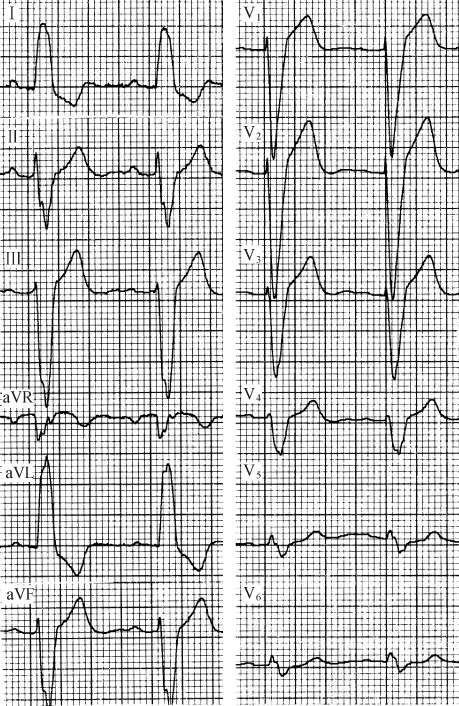
\includegraphics[width=3.10417in,height=4.77083in]{./images/Image00723.jpg}
 \captionsetup{justification=centering}
 \caption{曾有心肌梗死病史患者,出现完全性左束支阻滞伴电轴左偏、前侧壁r波振幅逆递增或递增不良并出现S、s波,提示前侧壁陈旧性心肌梗死(V\textsubscript{1}~V\textsubscript{6} 导联定准电压均为0.5mV)}
 \label{fig44-15}
  \end{figure} 


(7)若V\textsubscript{2} ~V\textsubscript{6}
导联尤其是V\textsubscript{4} ~V\textsubscript{6}
导联呈现明显切迹的QS型或(和)QRS电压明显降低(低于肢体导联),则提示合并广泛前壁梗死。

(8)若Ⅱ、Ⅲ、aVF导联QRS电压显著降低,出现q波及终末S波,则提示合并下壁梗死。

上述QRS波群改变,如同时伴有特征性ST-T改变及演变规律,则诊断意义更大。

2.下壁心肌梗死合并左前分支阻滞

左前分支阻滞时,QRS初始0.02s向量位于左下;而下壁心肌梗死时,QRS初始0.02s向量则位于左上;两者并存时,可互相影响QRS波群的典型表现,下列两点有助于两者并存的诊断:

(1)QRS波群改变:①左前分支阻滞掩盖下壁梗死(仅累及下壁前部),具有左前分支阻滞的特点,Ⅱ、Ⅲ、aVF导联呈rS型,若r\textsubscript{Ⅲ}
>r\textsubscript{aVF} >r\textsubscript{Ⅱ}
,Ⅱ导联r波若呈双峰或其前有q波,则提示合并下壁梗死;②大面积下壁梗死(累及全下壁)掩盖左前分支阻滞,Ⅱ、Ⅲ、aVF导联呈QS型,若Ⅱ、Ⅲ、aVF导联S波不降低(即S波仍较深),且无终末R波,则提示合并左前分支阻滞。

(2)特征性ST-T改变和演变:Ⅱ、Ⅲ、aVF导联出现ST段损伤型抬高,是诊断合并下壁急性梗死的有力证据。

此外,少数左前分支阻滞在V\textsubscript{1} 、V\textsubscript{2}
导联可出现q波,呈qrS型,酷似前间壁陈旧性心肌梗死,但低一肋间描记,q波即消失,应注意鉴别。

3.心肌梗死合并预激综合征

预激综合征影响QRS初始向量,正向δ波将掩盖心肌梗死的Q波,而负向δ波则酷似心肌梗死的Q波。以下三点可提示或疑有预激综合征合并急性心肌梗死:

(1)以R波为主导联出现ST段抬高。

(2)以S波为主导联出现倒置或深尖的T波。

(3)ST-T有动态演变。

急性损伤性ST-T动态演变(具有定位意义),结合临床症状、心肌酶谱、肌钙蛋白阳性是确诊预激综合征合并急性心肌梗死的主要依据(图\ref{fig36-16})。对合并陈旧性心肌梗死的定位诊断只有消除δ波或诱发顺向型折返性心动过速时,方能明确诊断。

4.心肌梗死合并右束支阻滞

两者图形能同时显现,但前间壁急性梗死时,右束支阻滞的继发性ST段压低将会影响ST段抬高程度,使其抬高程度减轻或回到基线形成伪善性改变。

5.心肌梗死合并左后分支阻滞

(1)下壁梗死合并左后分支阻滞:①电轴右偏(>+110°);②Ⅱ、Ⅲ、aVF导联QRS波群呈QR型,R\textsubscript{Ⅲ}
>R\textsubscript{aVF} >R\textsubscript{Ⅱ} ,Ⅰ、aVL导联呈rS型。

(2)前侧壁梗死合并左后分支阻滞:①Ⅰ、aVL导联QRS波群呈QS型;②Ⅱ、Ⅲ、aVF导联初始q波消失,出现R波,且R\textsubscript{Ⅲ}
>R\textsubscript{aVF} >R\textsubscript{Ⅱ} 。

6.急性心肌梗死合并室性异位心律时的诊断

(1)室性异位QRS波群的特殊形态:在左心室外膜面导联(V\textsubscript{1}
、aVR导联除外),若室性异位QRS波群呈qR、QR、qRs、QRs型,则提示存在心肌梗死;若呈QS型QRS波群时间增宽(≥0.18s),QS波中有>0.05s的挫折,特别是其后伴有ST段呈弓背向上型抬高时,也应考虑心肌梗死。

(2)出现原发性ST-T改变:①出现与QRS主波同向的ST段抬高或以负向波为主时其ST段呈弓背向上型抬高,均提示急性心肌梗死;②T波顶峰变尖,两肢对称呈帐篷状或冠状T波时,可能是心肌梗死最早期的征象。

7.急性心肌梗死合并心室人工起搏心律时的诊断

(1)以R波为主导联出现ST段抬高≥0.1mV或伴T波高耸。

(2)以S波为主导联出现ST段抬高≥0.5mV伴T波高耸,敏感性53\%,特异性88\%。

(3)以S波为主导联ST段压低≥0.1mV或伴T波倒置,敏感性29\%,特异性82\%。

(4)以上ST-T改变呈动态改变时,其诊断价值更大。

\protect\hypertarget{text00052.htmlux5cux23subid630}{}{}

\subsection{心肌梗死并发症的心电图改变}

急性心肌梗死后所出现的并发症主要包括急性心力衰竭、心源性休克、心律失常、梗死后综合征、心脏破裂及室壁瘤形成等。本文着重讨论后4种并发症的心电图改变。

1.心律失常

(1)缺血性心律失常(冠状动脉闭塞性心律失常):可分为梗死后早期心律失常(冠状动脉闭塞后数分钟至0.5h内发生)和后期心律失常(冠状动脉闭塞后4~48h内发生),而冠状动脉闭塞后0.5~4h内很少有心律失常发生,则称为寂静期。早期心律失常以折返机制为主,晚期以自律性增高为主,多表现为室性早搏、短阵性室性心动过速,并易恶化为心室颤动,部分患者可表现为房性早搏、短阵性房性心动过速、心房颤动等房性心律失常和缓慢性心律失常(如窦性心动过缓、窦性停搏)及传导阻滞(如房室传导阻滞、心室内传导阻滞等)。

(2)再灌注心律失常(请见本章下面的内容)。

2.梗死后综合征

(1)基本概念:急性心肌梗死后坏死的心肌和心包的抗原与抗体免疫系统产生自身免疫反应,引起心包腔内无菌性炎症伴液体渗出。通常发生在梗死后2~3周内。

(2)心电图改变:①多数导联又出现ST段突然抬高,但程度较轻;②原倒置T波可转为直立或双向;③可出现PR段抬高;④心包大量积液时,出现QRS波幅低电压,可伴有QRS、ST、T各波段电交替现象。

3.心脏破裂

心脏破裂是急性心肌梗死最严重的并发症之一,常发生在透壁性心肌梗死的第1周内,尤其是第1天内最为常见,严重者可引起猝死。

(1)左心室游离壁破裂:常发生急性心包填塞而猝死。

(2)室间隔穿孔:见于室间隔透壁性梗死,如穿孔较小,仅表现为前间壁急性梗死图形;如穿孔较大,可出现右心室容量负荷增加的心电图改变。

(3)乳头肌断裂:可造成二尖瓣关闭不全,出现左心室容量负荷增加的心电图改变。

4.室壁瘤形成

(1)基本概念:指梗死面积较大的急性透壁性心肌梗死灶愈合过程中被结缔组织所取代,受心室腔压力的作用,梗死区心室壁向外呈袋状、囊状或不规则状膨出。发生率约10\%~30\%,能引起心功能不全、恶性室性心律失常、血栓形成等多种并发症,严重威胁患者的生命。

(2)形成原因:①梗死面积大;②透壁性梗死;③梗死区血管完全闭塞而无侧支循环形成。

(3)分类:按病理解剖分类:①真性室壁瘤:梗死灶被结缔组织所取代形成薄弱的瘢痕区,心脏收缩呈反向运动(矛盾运动);②假性室壁瘤:心肌梗死急性期心室壁已破裂,破口周围被血栓堵塞或粘连,瘤壁由心包膜组成。按病程分类:①急性室壁瘤:指心肌梗死发病后24h内形成的室壁瘤(实为坏死区坏死组织在心脏收缩向外膨出),易发生心脏破裂;②慢性室壁瘤:指心肌梗死发生15天后由结缔组织所取代而形成的室壁瘤。

(4)心电图改变:急性室壁瘤体表心电图难以诊断,而慢性室壁瘤体表心电图具有重要的预测和诊断价值,符合下列条件越多,诊断准确性越高:①ST段抬高至少出现在4个导联;②V\textsubscript{1}
~V\textsubscript{3} 导联ST段抬高≥0.2mV,V\textsubscript{4}
~V\textsubscript{6}
导联及以R波为主的肢体导联ST段抬高≥0.1mV持续1个月,或者≥0.2mV持续15天;③ST段抬高的导联有异常Q波;④运动试验时,在原有异常Q波导联上出现ST段呈弓背向上抬高≥0.1mV;⑤前壁梗死后V\textsubscript{3}
~V\textsubscript{5} 导联出现持续性ST段抬高伴V\textsubscript{1}
导联T波直立或低平,对诊断心尖部室壁瘤有较高特异性和准确性(图\ref{fig44-16})。

\begin{figure}[!htbp]
 \centering
 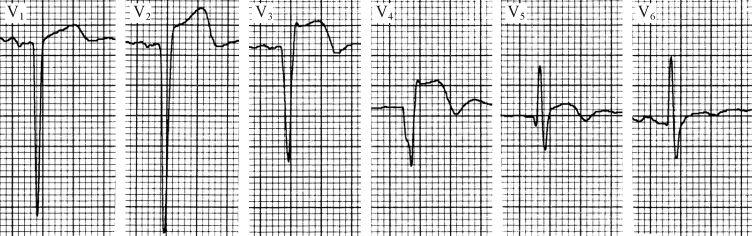
\includegraphics[width=5.08333in,height=1.59375in]{./images/Image00724.jpg}
 \captionsetup{justification=centering}
 \caption{陈旧性前间壁、前壁心肌梗死3年,V\textsubscript{2}~V\textsubscript{5} 导联出现持续性ST段抬高伴V\textsubscript{1}导联T波直立,心脏超声波显示心尖部室壁瘤形成}
 \label{fig44-16}
  \end{figure} 


\protect\hypertarget{text00052.htmlux5cux23subid631}{}{}

\subsection{再灌注治疗对急性心肌梗死转归的影响}

随着对急性心肌梗死早期诊断、早期实施溶栓、PTCA及放置支架等再灌注治疗,大多数患者将会缩小梗死面积、减少异常Q波发生率、缩短病程、改善预后,但少数患者反而出现再灌注损伤和心律失常,使病情加重,甚至危及生命。

1.再灌注治疗心肌血供改善有效性的心电图改变

再灌注治疗后,早期(3h内)主要观察ST段是否快速回落,随后的12~24h内,则主要观察T波变化。

(1)抬高ST段快速回落:再灌注治疗开始后2h内或相隔0.5h,抬高ST段快速回落≥50\%,或者ST段回落>0.2mV,或者再灌注3h内ST段回落>25\%,以上改变均属ST段早期快速回落。3~24h之间仍有一部分ST段缓慢回落,72h达较稳定水平。ST段早期快速回落是心肌再灌注成功的指标,若ST段完全回落(早期回落≥70\%或ST段抬高<0.1mV)所需时间愈短、幅度愈大,则预后愈好。

(2)不出现异常Q波或Q波消失或变小:成功的再灌注治疗,约有1/3患者ST段抬高导联不出现异常Q波,部分Q波消失或变小。

(3)加速T波演变:成功的再灌注治疗将加速T波演变,可使T波出现两次加深的演变。①直立高耸的T波振幅明显降低;②24h内ST段抬高导联出现早期T波倒置,为心肌再灌注成功的表现,是梗死相关动脉再通的独立指标;③两次T波倒置加深演变:第1次最深出现在再灌注后48~72h,提示有较多心肌细胞获救,变浅几天后再加深,第2次最深出现在梗死后2~4周;④以后T波倒置深度又逐渐变浅直至恢复正常,预示梗死区“冬眠”心肌功能恢复,T波转为直立时间越早,左心室功能恢复越好。

(4)原有的心律失常减轻或消失。

2.再灌注性损伤

(1)基本概念:指心肌严重缺血持续一段时间再恢复血液灌注后,反而出现缺血性损伤进一步加重的病理现象,表现为心肌结构破坏和心功能损害更为明显,是一种严重的治疗矛盾,将影响治疗效果,甚至危及生命。

(2)发生机制:缺血性损伤是再灌注损伤发生、发展的基础,再灌注恢复供血后产生大量氧自由基、细胞内Ca\textsuperscript{2+}
超载、白细胞炎性反应作用及高能磷酸化合物缺乏等原因直接引起心肌细胞损伤、死亡及微循环出现无复流现象加重心肌缺血性损伤。

(3)影响因素:①缺血时间:再灌注损伤易发生在缺血性心肌可逆性损伤期内(一般在缺血15~45min后发生的再灌注);②侧支循环:急性心肌梗死后,如易于建立侧支循环,则不易发生再灌注损伤;③再灌注条件:如低压、低温(25℃)、低pH值、低钠、低钙液灌流,可使再灌注损伤减轻、心功能迅速恢复,反之,则可诱发或加重再灌注损伤;④缺血范围:当缺血面积>20\%时,再灌注损伤发生率高;⑤再灌注的血流速度:当血流速度快,冲洗作用强时,其发生率就高;⑥再灌注区可逆性心肌细胞数量多时,其发生率高。

(4)临床及心电图特征:①临床症状(如胸痛等)持续加重或缓解后出现反弹和加重、心肌酶谱持续增高;②ST段持续性抬高、进行性抬高或回落后再次抬高(>0.1mV);③出现再灌注性心律失常;④心肌坏死面积增加导致异常Q波出现的导联数增多,再灌注治疗后6h或第1天的死亡率增加。

3.再灌注性心律失常

再灌注性心律失常的发生率高达80\%,以心肌血供中断15~45min后的再灌注,特别是再灌注后的5min内,心律失常发生率最高,以非阵发性室性心动过速(或加速的室性逸搏心律)、成对室性早搏、短阵性室性心动过速多见,严重者可发生心室颤动而死亡,也可出现缓慢性心律失常,如窦性心动过缓、窦性停搏及房室传导阻滞等。

再灌注性心律失常的发生机制有:①可逆性心肌细胞与正常心肌细胞之间电生理异常引起折返;②再灌注时的冲洗现象,使堆积的乳酸、儿茶酚胺入血,引起自律性增高;③细胞内Ca\textsuperscript{2+}
超载,引起触发活动。

4.持续性ST段抬高的临床意义

(1)再灌注治疗早期ST段未能快速回落,持续在较高水平,是心肌水平未得到再灌注的表现。

(2)ST段进行性抬高伴临床症状加重,提示病情进展,可能存在梗死灶延伸、毗邻梗死区再梗死或再灌注性损伤。

(3)24h后ST段再抬高,应警惕再梗死的发生。

(4)ST段持续抬高2周以上,应警惕室壁瘤形成的可能(图\ref{fig44-17})。

\begin{figure}[!htbp]
 \centering
 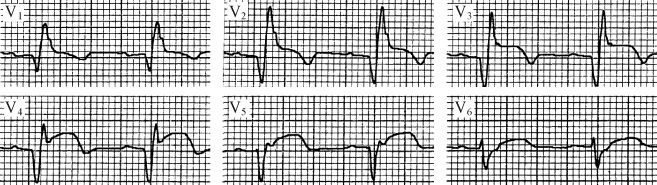
\includegraphics[width=4.4375in,height=1.25in]{./images/Image00725.jpg}
 \captionsetup{justification=centering}
 \caption{女性,84岁,前间壁、前壁心肌梗死1年余。显示完全性右束支阻滞、前间壁及前壁异常Q波伴ST段抬高,提示室壁瘤形成(被心脏超声波证实)}
 \label{fig44-17}
  \end{figure} 

\protect\hypertarget{text00052.htmlux5cux23subid632}{}{}

\subsection{心肌梗死面积的心电图评估}

1.QRS计分法(Wanger法)

(1)原理:急性心肌梗死后异常Q波和R波改变的导联数量越多,则梗死面积越大。QRS计分法就是利用常规12导联心电图加权计分系统评价心肌梗死面积总百分比的方法。

(2)基本要求:①必须是室上性节律,心室率<120次/min;②基线稳定,足以准确测量QRS波群各波的时间和电压;③必须是12导联同步记录,至少是6个导联同步;④Q波时间准确测量极为重要。

(3)基本方法:先除去Ⅲ、aVR导联,计算剩余10个导联的Q波和R/Q振幅比的变化而计分(表44-1),将计分结果代入以下公式计算:前壁梗死面积(\%)=3.6×计分值+3.2,下壁梗死面积(\%)=2.5×计分值+2.9。

\begin{table}[htbp]
\centering
\caption{简化的心肌梗死面积QRS计分法}
\label{tab44-1}
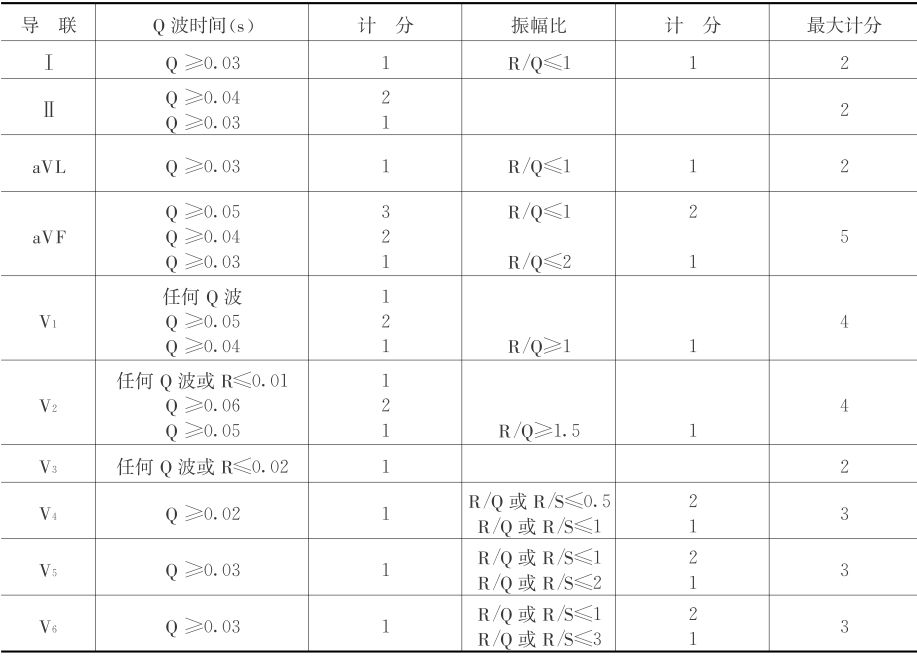
\includegraphics[width=6.19792in,height=4.42708in]{./images/Image00726.jpg}
\end{table}

(4)评价:QRS计分法需在梗死后1周、梗死范围相对稳定时应用,对前壁急性心肌梗死面积的评估最佳,其次为下壁、后侧壁。QRS计分与急性心肌梗死患者预后显著相关,当QRS计分≥10分时(约30\%左心室梗死),患者1月、1年的病死率增加。QRS计分对前壁陈旧性梗死面积也有较好的评估价值。

2.ST段总抬高计分法(Aldrich计分法)

(1)方法:计算ST段抬高的导联数及抬高值的总和,对梗死面积进行评估。前壁梗死面积(\%)=3×(1.5×ST段抬高导联-0.4),下壁梗死面积(\%)=3×(0.6×下壁导联ST段抬高值的总和+2)

(2)评价:Aldrich计分法简便实用,对梗死面积有半定量的价值,可预测左心室功能、心肌再灌注治疗的疗效。

3.综合ST段抬高、QRS波和T波改变(Wikins法)

(1)方法:计算ST段抬高的导联数、抬高值的总和、异常Q波的导联数、异常Q波时间总和及T波高耸的导联数。其中异常Q波标准为Ⅰ、Ⅱ、aVL、aVF、V\textsubscript{5}
、V\textsubscript{6} ≥0.03s,V\textsubscript{4}
≥0.02s,V\textsubscript{1} ~V\textsubscript{3}
导联出现Q波;T波高耸标准为Ⅱ≥0.6mV,Ⅲ、aVL≥0.3mV,Ⅰ、aVF、V\textsubscript{1}
≥0.45mV,V\textsubscript{2} ≥1.1mV,V\textsubscript{3}
≥1.5mV,V\textsubscript{4} ≥1.2mV,V\textsubscript{5}
≥0.9mV,V\textsubscript{6}
≥0.65mV。前壁梗死范围=1.88×ST段抬高导联数+2.19×异常Q波导联数+1.56×T波高耸导联数+5.8,下壁梗死范围=0.94×ST段抬高总和+1.13×Q波时间总和+8.73。

(2)评价:对前壁梗死面积的评估价值较大,对下壁梗死面积的评估需进一步完善。

4.根据梗死灶大小、临床及病理所见,可将心肌梗死分为局灶性梗死(显微镜下梗死)、小面积梗死(<左心室的10\%)、中面积梗死(左心室的10\%~30\%)、大面积梗死(>左心室的30\%)。

\protect\hypertarget{text00052.htmlux5cux23subid633}{}{}

\subsection{心电图及其相关检查判断急性心肌梗死病情及预后的价值}

急性心肌梗死患者的病情及预后,主要取决于梗死的范围和部位,这又受以下5个因素的影响:①冠状动脉阻塞部位及其持续时间;②开始时心肌缺血的范围;③缺血区侧支循环建立情况;④缺血区心肌代谢情况;⑤早期再灌注治疗的有效性和有无再灌注损伤出现。常规心电图检查具有简便、快捷、经济、无创及可反复检查等优点,不仅可以确定急性心肌梗死的诊断,还能判断梗死部位,并进行分期,根据心电图演变情况可对心肌梗死患者的病情及预后进行评估,指导临床治疗。

1.急性心肌梗死患者病情重、预后差的心电图表现

有下列心电图改变者,提示急性心肌梗死患者病情重、预后差:

(1)出现墓碑型ST段抬高:该心肌梗死以老年人多发。均发生在穿壁性心肌梗死中,入院1周内并发症多,如循环衰竭、严重心律失常、三度房室传导阻滞/束支阻滞、心肌梗死后心绞痛及扩展明显增多,死亡率显著增高,是急性心肌梗死近期预后险恶的独立指标。

(2)急性心肌梗死出现新发的左束支阻滞、不定型心室内传导阻滞、房室传导阻滞:并不是新发生的各种传导阻滞使患者的病情迅速加重,而是新发生的各种传导阻滞代表着病情在进展、梗死面积在扩大。因此,新发生的各种传导阻滞都提示左心室前壁和前降支受累、梗死还在发展和面积在扩大、患者的预后差,死亡率可增加40\%~60\%,心源性休克的发生率高达70\%以上。

(3)急性前壁心肌梗死出现新发的右束支阻滞:为大面积心肌梗死的表现,常伴有心力衰竭、三度房室传导阻滞、心室颤动和高死亡率。

(4)急性前壁心肌梗死伴任一导联ST段压低:梗死后发生再梗死、心力衰竭、室性心律失常等心脏事件增多,其远期病死率高。

(5)急性前壁心肌梗死伴ST段持续抬高、T波直立;前壁急性梗死后2~5天内ST段仍持续抬高伴T波直立,高度提示左心室内有血栓形成(敏感性96\%,特异性93\%)。

(6)急性前侧壁心肌梗死伴aVR导联ST段压低:提示心肌梗死面积较大,CK-MB峰值较高,心功能较差,LVEF≤35\%,心力衰竭发生率高。

(7)急性下壁心肌梗死伴左胸导联(V\textsubscript{4} ~V\textsubscript{6}
)ST段压低:多伴有前降支病变,且右冠状动脉近端阻塞及合并三支冠状动脉病变发生率高,为冠状动脉病变严重而广泛且侧支循环差的表现;同时,其左心室功能也差,并发症亦多,预后较差,住院期间的病死率可达41\%。

(8)急性下壁心肌梗死患者在下壁导联出现高耸T波而ST段抬高不明显或抬高<0.1mV,同时出现左胸导联ST段压低,表明既往有过梗死或同时伴有前壁心肌缺血,属极高危型患者,住院期间的病死率可高达69\%。由此可见,下壁心肌梗死患者预后主要取决于前壁心肌缺血情况。

(9)下壁急性心肌梗死伴aVR导联ST段压低:表明心肌梗死面积较大,CK-MB峰值较高,住院率和1年并发症发生率增高。

(10)广泛导联出现既宽又深的异常Q波,表明梗死范围广、厚度深呈透壁性梗死,易形成室壁瘤或心脏破裂而猝死,如广泛前壁心肌梗死。

(11)出现持续性或进行性ST段抬高:早期见于梗死灶延伸、毗邻梗死区再梗死或再灌注性损伤,提示病情进展或进行性加重;若持续抬高2周以上,提示室壁瘤形成,容易导致心功能不全、恶性室性心律失常、血栓形成等多种并发症,严重威胁患者的生命。

(12)急性心肌梗死半年后T波仍持续倒置:预示透壁性坏死,左心室功能恢复差,远期预后差。

(13)再灌注治疗后出现持续性ST段再抬高:是心肌再次损伤的标志,见于冠状动脉再闭塞、梗死面积扩大、再灌注损伤及侧支循环较差等情况,再灌注治疗后6h或第1天的死亡率增加,左心室功能恢复较差,远期病死率增加。

(14)再发性心肌梗死:患者左心室功能恢复较差,近期与远期病死率均增加。

(15)急性心肌梗死伴T波电交替:多见于心肌缺血、心功能不全、电解质紊乱等患者。有T波电交替者,发生致命性室性心律失常的危险性增加14倍。T波电交替已成为识别高危患者的一个重要而非常直观的指征。

(16)出现严重的心室内传导阻滞(QRS波群时间>0.16s):当窦性QRS波群呈左、右束支阻滞型或不定型心室内传导阻滞时或室性异位搏动的QRS波群时间>0.16s,称为特宽型QRS波群。QRS波群宽度与心室负荷程度及心肌病变严重程度相关,具有诊断及预后的意义,多见于严重的器质性心脏病患者,尤其是老年冠心病患者。现已证明,完全性左束支或右束支阻滞,均为独立的危险因素。

(17)出现严重的快速性心律失常:各种类型的室性心动过速、阵发性室上性心动过速、心房颤动或扑动伴极快的心室率等,最终易导致心室扑动、颤动而猝死。

(18)出现严重的缓慢性心律失常:病窦综合征、持久性或阵发性三度房室传导阻滞伴心室停搏,尤其是较长时间的心室停搏(>5.0s)或短时间内出现高频度的心室停搏等,易发生阿-斯综合征而猝死。

(19)出现复杂性室性心律失常:频发成对的、多源性、多形性、特宽型(时间>0.16s)、特矮型(振幅<1.0mV)及Ron-T、Ron-P的室性早搏,易诱发室性心动过速或心室颤动而危及生命。

(20)出现严重的慢-快型综合征:在各种缓慢性心律失常的基础上,出现阵发性心房颤动、扑动、室上性心动过速、室性心动过速等快速性心律失常,易导致心力衰竭或加重心力衰竭。

(21)出现严重的快-慢型综合征:阵发性心房颤动、扑动、室上性心动过速、室性心动过速等快速性心律失常发作终止时,在恢复窦性心律之前,出现长R-R间歇,易发生晕厥、阿-斯综合征而猝死。

(22)出现心室电分离现象:多见于垂危心脏病患者的临终期或严重器质性心脏病患者,是一种不可逆的病理现象,它使血流动力学及冠状动脉灌注严重恶化,进而导致心肌缺血,在心肌的不同层次发生碎裂波,表现心电离散。故心室分离提示心肌病变严重而广泛,预后极差。

(23)心室晚电位阳性:表明心室内存在潜在的折返环,是产生折返性室性心动过速的电生理基础,易引发致命性室性心律失常,对心肌梗死患者的预后预测、冠心病、心力衰竭患者猝死危险性预测有重要意义。

(24)心率变异性(HRV)异常:自主神经系统与心源性猝死密切相关,心电稳定性有赖于交感、副交感神经和体液调节之间的平衡。若交感神经张力过度增高,则有利于致命性心律失常的发生;而副交感神经激活,则具有保护心脏和抗心室颤动作用。其中SDNN反映交感与副交感神经总的张力大小,SDANN、SDNN\textsubscript{index}
值降低,表明交感神经张力增高;而r-MSSD、PNN\textsubscript{50}
值降低,则表明副交感神经张力降低,如SDNN<50ms者的死亡相对危险性高出SDNN>100ms者5倍;心肌梗死后6~12个月HRV仍不能恢复正常者,则提示预后不佳。

(25)窦性心律震荡现象不明显或消失:见于心肌梗死后猝死的高危患者。震荡初始(TO)、震荡斜率(TS)指标对猝死高危患者预测作用稳定而可靠,两者均异常时,是猝死最敏感的预测指标,其阳性预测精确度达32\%,同时阴性预测精确度达90\%。

(26)心脏变时性功能不全:运动试验中无ST段压低而有变时性功能不全者,经冠状动脉造影,72\%患者有明显的冠状动脉病变;运动试验中有ST段压低伴变时性功能不全者,冠状动脉三支病变的发生率高于仅有ST段压低者。提示运动试验中变时性功能不全是诊断冠心病的一个独立而敏感的阳性指标,也是冠心病事件(如心绞痛、心肌梗死、猝死)发生风险及预后判断指标之一。

2.急性心肌梗死预后较好的心电图表现

(1)急性前壁心肌梗死伴V\textsubscript{4} ~V\textsubscript{6}
导联U波倒置:约30\%急性前壁梗死患者出现V\textsubscript{4}
~V\textsubscript{6}
导联U波倒置,与无U波倒置患者比较,前者心肌坏死面积较少,左心室功能较好,故急性前壁梗死时出现U波倒置是预后较好的一个心电图指标,与侧支循环较丰富有关。

(2)急性前壁心肌梗死伴V\textsubscript{4} ~V\textsubscript{6}
导联巨倒T波:急性前壁梗死后5天内,V\textsubscript{4}
~V\textsubscript{6}
导联如出现巨倒T波(深度≥1.0mV),则预示有R波重现可能和较好的左心室功能,预后较佳。

(3)急性心肌梗死早期再灌注治疗后2h内抬高ST段快速回落≥50\%或完全回落(回落≥70\%或ST段抬高<0.1mV),是心肌组织水平再灌注的客观指标,ST段快速回落或完全回落所需时间愈短,回落幅度愈大,则心肌组织水平再灌注愈好,左心室收缩功能恢复愈佳,近、远期死亡率愈低。

(4)再灌注治疗后ST段抬高导联未出现异常Q波或q波较小较浅。

(5)再灌注治疗后24h内ST段抬高导联出现早期T波倒置:是心肌组织再灌注成功的心电图表现,是梗死相关动脉再通的独立指标,并与住院期间存活率相关;T波倒置愈深,提示有较多的心肌获救,心功能恢复较好,是慢性期左心室壁运动异常恢复的预测指标。

(6)心肌梗死后,倒置T波转为直立的时间越早,则左心室功能恢复越好,预后越佳。

\protect\hypertarget{text00052.htmlux5cux23subid634}{}{}

\subsection{急性心肌梗死鉴别诊断}

(1)急性肺栓塞:急性肺栓塞临床上可出现胸痛、呼吸困难,心电图出现S\textsubscript{Ⅰ}
Q\textsubscript{Ⅲ} T\textsubscript{Ⅲ} 型及V\textsubscript{1}
~V\textsubscript{3}
导联ST段抬高、T波倒置,应与急性下壁、前间壁心肌梗死相鉴别。但前者常出现窦性心动过速、肺型P波、电轴右偏、显著的顺钟向转位及一过性右束支阻滞,且ST段抬高程度较轻,心肌酶谱正常或轻度增高,而后者ST段明显抬高,心肌酶谱明显升高。

(2)急性心包炎:患者有胸痛、ST段抬高,需与急性心肌梗死相鉴别。具体鉴别请见第四十二章第七节急性心包炎。

(3)变异型心绞痛:患者有胸痛、硝酸甘油不能缓解,ST段抬高伴T波高耸,酷似急性心肌梗死,但变异型心绞痛用Ca\textsuperscript{2+}
拮抗剂治疗有效,随着症状的缓解,ST-T逐渐恢复正常,心肌酶谱正常范围。若病情进一步发展,且不能缓解,则很可能发展为急性心肌梗死。

(4)早复极综合征合并变异型心绞痛:患者有胸痛,硝酸甘油不能缓解,ST段显著抬高伴T波高耸,酷似急性心肌梗死,但前者心肌酶谱正常范围,Ca\textsuperscript{2+}
拮抗剂治疗有效。

(5)早复极综合征:患者有ST段抬高伴T波高耸,若伴有其他原因引起的胸痛,有时易误诊为变异型心绞痛或急性心肌梗死,但前者多见于年轻身体素质良好者,平时心率较慢,活动后或心率加快后ST段抬高程度减轻或恢复正常,心肌酶谱正常。

(6)急性重症心肌炎(暴发型心肌炎):少数重症心肌炎患者起病急骤,病情凶险,出现异常Q波、ST段呈损伤型抬高、心肌酶谱增高酷似急性心肌梗死。一般地说,年轻患者,发病前有感染史,既往无心脏病史,以暴发型心肌炎可能性为大,冠状动脉造影有助两者的鉴别。

(7)肥厚型心肌病:部分患者出现异常Q波、显著ST段压低及T波倒置,类似冠状T波,酷似急性心内膜下心肌梗死,但前者异常Q波多表现为深而窄的Q波,时间不增宽,心肌酶谱正常,心脏超声波检查可资鉴别。

(8)心脏肿瘤:较大的心脏肿瘤其所对应的导联可出现异常Q波、ST段抬高酷似急性心肌梗死,心肌酶谱、肌钙蛋白、心脏超声波及核磁共振检查可资鉴别(图\ref{fig44-18})。

\begin{figure}[!htbp]
 \centering
 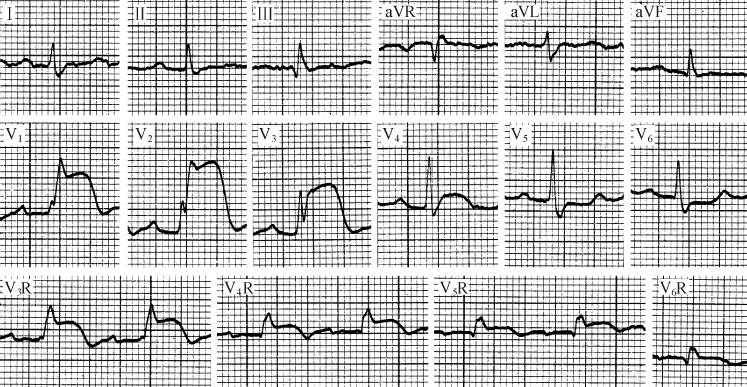
\includegraphics[width=5.04167in,height=2.61458in]{./images/Image00727.jpg}
 \captionsetup{justification=centering}
 \caption{女性,70岁,心脏超声波诊断右心室肿瘤。心电图显示房室传导延缓(P-R间期0.22s)、不完全性右束支阻滞、V\textsubscript{3}R~V\textsubscript{6} R、V\textsubscript{1} ~V\textsubscript{4}导联持续性ST段抬高、前侧壁轻度ST段改变、下壁轻度T波改变}
 \label{fig44-18}
  \end{figure} 


(9)高钾血症:血钾过高可导致部分心肌细胞膜的静息电位低于阈电位而出现“电静止”现象,产生可逆性异常Q波;此外,血钾过高可产生损伤电流样改变出现ST段抬高,酷似急性心肌梗死的心电图改变(图\ref{fig44-19})。但当血钾恢复正常后,异常改变的心电图即恢复正常而有别于急性心肌梗死特有的ST-T动态演变规律。

\begin{figure}[!htbp]
 \centering
 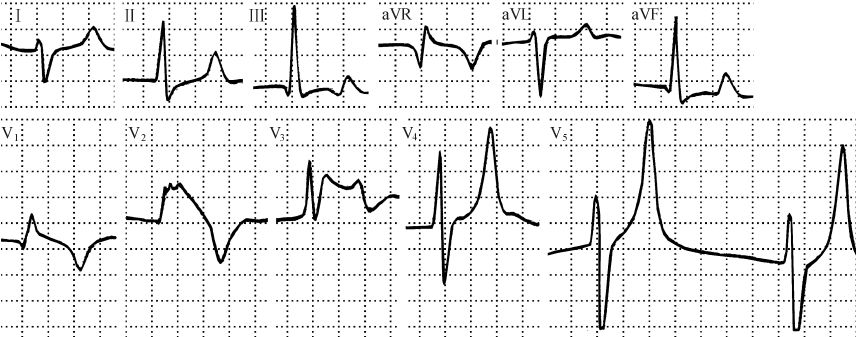
\includegraphics[width=5.78125in,height=2.27083in]{./images/Image00728.jpg}
 \captionsetup{justification=centering}
 \caption{男性,68岁,尿毒症、高钾血症(8.6mmol/L)患者。心电图显示显著的窦性心动过缓伴窦-室传导、左后分支阻滞(电轴由原来的+58°增至+107°)、不定型心室内传导阻滞、前间壁异常Q波伴ST段损伤型抬高、T波高耸,符合高钾血症的心电图改变。治疗后血钾恢复正常,心电图亦恢复正常(引自张茜)}
 \label{fig44-19}
  \end{figure} 

(10)Brugada综合征或Brugada波:V\textsubscript{1} ~V\textsubscript{3}
导联ST段呈“穹隆型”或“马鞍型”抬高伴T波倒置或正负双向酷似急性前间壁心肌梗死,但Brugada综合征或Brugada波有家族性遗传特点,多见于年轻人,一般情况尚好,心肌酶谱正常可资鉴别。

\protect\hypertarget{text00053.html}{}{}

\protect\hypertarget{text00053.htmlux5cux23chapter53}{}{}

\chapter{电解质异常的心电图改变}

\protect\hypertarget{text00053.htmlux5cux23subid635}{}{}

\section{电解质与心肌细胞特性的关系}

心肌细胞具有自律性、兴奋性、传导性、收缩性和舒张性5种生理特性,其中前三者属于电生理特性,是以心肌细胞膜的生物电活动为基础,由细胞内外各种离子不均匀分布及其跨膜运动所决定,与心电产生及心律失常发生有密切关系;而后两者则属于机械特性,与心脏泵血功能有关。

1.自律性

自律性是指心脏起搏细胞(主要为窦房结细胞和浦肯野细胞)自动发生节律性兴奋的特性。自律性的高低主要取决于4相舒张期自动除极化速率、最大舒张期电位及阈电位水平,用每分钟发放冲动的次数来衡量。凡是能加快4相自动除极化速率、缩小最大舒张期电位与阈电位水平之间的距离,均能提高自律性,如加快起搏细胞的Ca\textsuperscript{2+}
、Na\textsuperscript{+} 内流或延缓K\textsuperscript{+}
外流的因素;反之,均能降低自律性。

2.兴奋性

兴奋性是指心肌细胞受到刺激时产生兴奋的能力。用刺激阈值来衡量兴奋性的高低。刺激阈值高,表示兴奋性低;反之,则表示兴奋性高。它主要取决于细胞膜的静息电位或最大舒张电位的水平及引起0相除极化的离子通道性状。凡是能缩小细胞膜静息电位或最大舒张电位与阈电位水平之间的距离及增加静息状态的Na\textsuperscript{+}
通道数量(快反应细胞)、L型Ca\textsuperscript{2+}
通道数量(慢反应细胞),均能提高心肌细胞的兴奋性;反之,则降低心肌细胞的兴奋性。

心肌细胞兴奋性具有下列周期性改变:有效不应期、易颤期(仅指心房肌、心室肌)、相对不应期、超常期及应激期。

(1)绝对不应期(ARP)与有效不应期(ERP):前者是指从动作电位的0相开始到复极3相膜电位降至-55mV这一段时期,后者是指从动作电位的0相开始到复极3相膜电位降至-60mV这一段时期,对任何刺激均不发生反应。相当于QRS波群、ST段及T波顶峰之前的时间。

(2)相对不应期(RRP):是指有效不应期之后,膜电位从-60mV继续复极化到-80mV这一段时期,此时需要阈上刺激才能发生反应。相当于T波顶峰至T波结束的时间。

(3)易颤期:指在绝对不应期与相对不应期之间,各心肌细胞兴奋性的恢复不一致或不同步,此时若受到强刺激,极易发生纤维性颤动,称为易颤期。心房易颤期相当于R波降肢和S波时间内,心室易颤期相当于T波上升肢到顶峰前20~40ms,或在T波顶峰前30ms,约持续20~60ms。

(4)超常期:指相对不应期之后,膜电位从-80mV继续复极化到-90mV这一段时期,此时阈下刺激即能引起反应,称为超常期。相当于心电图中T波顶峰至U波结束的这段时间。

决定不应期长短的因素有:①膜电位水平;②心率因素:心率增快使心房肌、心室肌、房室旁道的不应期缩短,而房室结的不应期则在心率增快到一定程度时却反而延长;③解剖部位:房室结的不应期>心室肌>心房肌,右束支的不应期>左前分支>左束支>左后分支>左中隔支,90\%房室旁道的不应期>房室结(易出现顺向型房室折返性心动过速),90\%房室结快径路的不应期>慢径路(易出现慢-快型房室结内折返性心动过速);④年龄、性别:女性、年长者不应期长;⑤神经因素:迷走神经张力增高使房室结不应期延长,心房肌不应期缩短,而心室肌影响不大,交感神经张力增高,则使房室结不应期缩短;⑥药物因素。

3.传导性

传导性是指心肌细胞具有传导兴奋的能力。用传播速度来衡量传导性的高低。它主要取决于心肌细胞结构特点和电生理特性,前者与心肌细胞直径、细胞内的电阻大小及细胞间缝隙连接数量和功能状态有关,凡是细胞直径大、电阻小、缝隙连接数量多及处于开放状态,都能加快兴奋的传导;而后者则与0相除极化的速度和幅度及邻近未兴奋部位细胞膜的反应性有关,凡是能增加细胞膜的反应性、加大静息电位或最大舒张期电位水平(指负值加大)、降低阈电位水平(指负值加大,阈电位下移)及减少膜电阻和膜电容,均可提高兴奋传导的速度。

传导性根据动作电位时相可分为两类:

(1)0相传导:指邻近的心肌组织凭着0相除极所产生的电位差和电流依次除极的过程。

(2)2相传导:当部分心肌组织2相平台期消失,出现2相复极时的电位差和电流,引起邻近细胞依次除极的过程,可出现2相早搏、2相折返等心律失常,如Brugada综合征、特发性心室颤动患者发生的致命性心律失常都与2相传导、2相折返有关。

传导性根据电生理特性也可分为两类:

(1)快反应纤维(快反应细胞):含有快Na\textsuperscript{+}
通道,能快速传导冲动的心肌细胞,包括心房肌、心室肌、特殊的传导组织如结间束、希氏束、浦肯野纤维。其电生理特征:①静息膜电位负值大,约-80~-90mV;②0相上升速率快、幅度大,传导速度快;③含有快Na\textsuperscript{+}
通道,0相除极时离子流为Na\textsuperscript{+} ;④除极时阈电位为-65mV。

(2)慢反应纤维(慢反应细胞):含有慢Ca\textsuperscript{2+}
通道,缓慢传导冲动的心肌细胞,包括窦房结、房室结、冠状窦口邻近的心肌细胞。其电生理特征:①静息膜电位负值小,约-60~-70mV;②0相上升速率慢、幅度小,传导速度慢;③含有慢Ca\textsuperscript{2+}
通道,0相除极时离子流为Ca\textsuperscript{2+}
;④除极时阈电位为-30~-40mV。

4.收缩性和舒张性

心肌细胞兴奋时,通过兴奋-收缩耦联机制,触发心肌细胞收缩和随后的舒张,并与瓣膜的启闭相配合,造成心房和心室压力和容积的变化,从而推动血液在心血管系统内流动。心肌兴奋-收缩耦联主要与细胞内外Ca\textsuperscript{2+}
有关,但当血K\textsuperscript{+}
明显增高时,心房肌、心室肌将出现停止收缩而处于舒张状态。

5.动作电位

当心肌细胞受到刺激而兴奋时,细胞膜对离子的通透性发生了一系列的变化,出现一系列的离子跨膜运动,使膜内外的电位差发生迅速变化,称为动作电位。它包括除极化与复极化两个过程。每1次动作电位可分为5个时相:①0相除极化:与快Na\textsuperscript{+}
通道开放有关;②1相复极化:为快速复极化初期,与快Na\textsuperscript{+}
通道失活后,K\textsuperscript{+}
外流有关;③2相复极化:为缓慢复极化期,又称为平台期,与K\textsuperscript{+}
外流、Ca\textsuperscript{2+} 内流及少量Na\textsuperscript{+}
内流有关;④3相复极化:为快速复极化末期,与L型Ca\textsuperscript{2+}
通道失活后细胞膜对K\textsuperscript{+}
通透性急剧升高引起K\textsuperscript{+}
外流明显加快有关;⑤4相:又称为电舒张期、静息期或极化期,通过细胞膜上Na\textsuperscript{+}
-K\textsuperscript{+} 泵、Ca\textsuperscript{2+}
泵及Na\textsuperscript{+} -Ca\textsuperscript{2+}
交换体的活动,将细胞内的Na\textsuperscript{+} 、Ca\textsuperscript{2+}
排出,并将细胞外的K\textsuperscript{+}
摄入细胞内,以恢复细胞内外各种离子的正常浓度梯度,维持心肌细胞的正常兴奋性。

无论是心肌细胞的动作电位,还是自律性、兴奋性、传导性及收缩性都与Na\textsuperscript{+}
、K\textsuperscript{+} 、Ca\textsuperscript{2+}
等各种离子有关。一旦发生电解质紊乱,势必会影响心肌细胞的生理特性,引发各种心律失常、传导阻滞及心肌收缩性降低。心电图检查可为临床诊断、治疗提供重要价值。

\protect\hypertarget{text00053.htmlux5cux23subid636}{}{}

\section{血钾异常的心电图改变}

\protect\hypertarget{text00053.htmlux5cux23subid637}{}{}

\subsection{低钾血症}

1.基本概念

低钾血症是指血清钾浓度<3.5mmol/L的一种病理状态。可因钾摄入不足、排出过多或因稀释及转移到细胞内而导致血清钾浓度降低。

2.低钾血症对心肌细胞电生理的影响

正常人体内的K\textsuperscript{+}
主要分布在细胞内,为细胞外K\textsuperscript{+}
浓度的30倍。当血K\textsuperscript{+}
稍有减少(低钾血症早期),即可使细胞内、外K\textsuperscript{+}
浓度差更加显著,使细胞膜静息电位负值增大,细胞处于超极化状态,静息电位与阈电位之间的距离增大,导致心肌细胞的自律性和兴奋性降低;但随着血K\textsuperscript{+}
的进一步降低,细胞膜对K\textsuperscript{+}
的通透性降低,最终结果是静息电位负值轻度减少,一方面使0相除极化速度和幅度下降,传导性略降低,出现轻度的传导阻滞(如心房内传导阻滞、房室传导阻滞、束支阻滞等),另一方面缩短了与阈电位水平之间的距离,使心肌细胞自律性与兴奋性均增高;此外,由于3相阶段K\textsuperscript{+}
逸出减慢,复极时间延长,导致动作电位时间延长,超常期延长,尤其是浦肯野纤维动作电位时间延长的程度超过心室肌,使Q-T间期延长、T波低平及U波增高,也导致浦肯野纤维与心室肌的复极离散度增大,有利于产生早期后除极及折返而引起室性心律失常。

综上所述,低钾血症早期,心肌细胞自律性和兴奋性降低,而传导速度影响不明显;当缺钾进一步加重时,则使心肌细胞自律性和兴奋性增高,传导速度减慢,出现传导阻滞、心室内折返现象及早期后除极而引发室性心律失常。

3.心电图特征

(1)U波增高,T-U波融合,U波振幅>0.2mV或U波振幅>T波振幅,血K\textsuperscript{+}
越低,U波改变越明显,甚至出现巨大U波。

(2)T波增宽伴切迹,振幅降低。

(3)ST段多呈下斜型压低。

(4)Q-T间期或Q-U间期延长。

(5)心律失常:以多源性、多形性室性早搏、短阵性室性心动过速多见,有时出现尖端扭转型室性心动过速等恶性室性心律失常。

(6)传导阻滞:可出现不完全性心房内传导阻滞、房室传导阻滞、束支阻滞等(图\ref{fig45-1}、图\ref{fig45-2}、图\ref{fig45-3})。

\begin{figure}[!htbp]
 \centering
 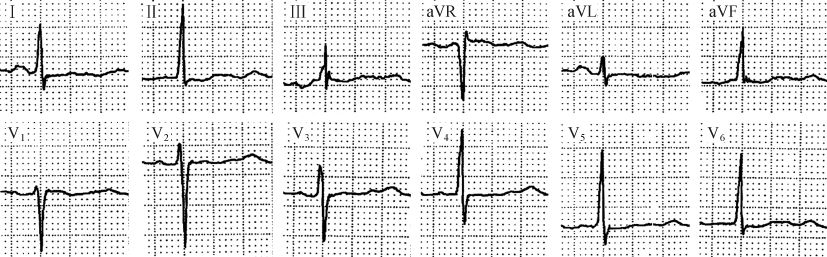
\includegraphics[width=5.58333in,height=1.72917in]{./images/Image00729.jpg}
 \captionsetup{justification=centering}
 \caption{周期性麻痹、低钾血症患者(血K\textsuperscript{+}3.1mmol/L),出现窦性心律伴P电轴左偏、T波及U波改变、Q-T间期延长、符合低钾血症的心电图改变}
 \label{fig45-1}
  \end{figure} 


\begin{figure}[!htbp]
 \centering
 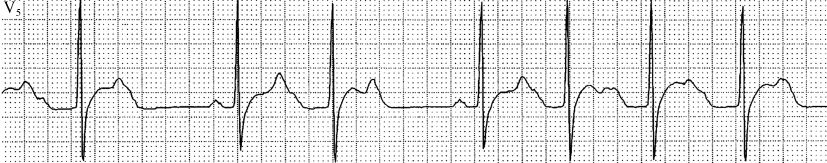
\includegraphics[width=5.58333in,height=1.09375in]{./images/Image00730.jpg}
 \captionsetup{justification=centering}
 \caption{低钾血症患者(血K\textsuperscript{+}2.9mmol/L),V\textsubscript{5}导联出现二度Ⅰ型房室传导阻滞呈3:2~5:4传导、T波与U波融合、Q-U间期延长}
 \label{fig45-2}
  \end{figure} 


\begin{figure}[!htbp]
 \centering
 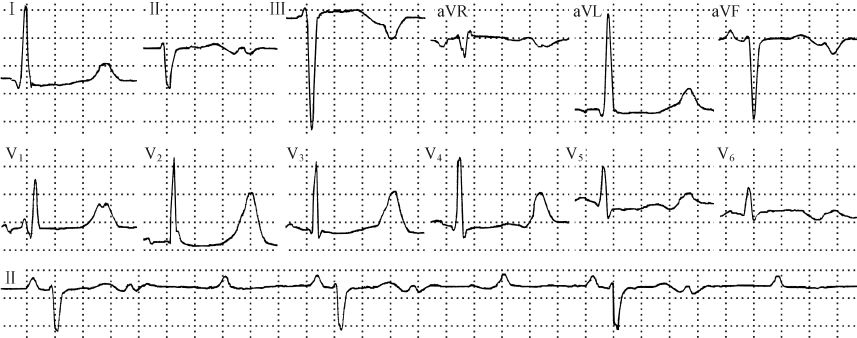
\includegraphics[width=5.79167in,height=2.28125in]{./images/Image00731.jpg}
 \captionsetup{justification=centering}
 \caption{周期性麻痹、低钾血症患者(血K\textsuperscript{+}2.6mmol/L),出现三支阻滞(完全性右束支阻滞、左前分支阻滞、左后分支二度阻滞呈3:1传导)、肢体导联左心室高电压、T波及U波改变、Q-T间期延长、符合低钾血症的心电图改变}
 \label{fig45-3}
  \end{figure} 


\protect\hypertarget{text00053.htmlux5cux23subid638}{}{}

\subsection{高钾血症}

1.基本概念

高钾血症是指血清钾浓度>5.5mmol/L的一种病理状态。多见于急、慢性肾功能衰竭、溶血性疾病、挤压综合征、大面积烧伤、输血过多等。一旦出现高钾血症,预后严重,如不及时处理,常危及生命。

2.高钾血症对心肌细胞的影响

(1)对心肌细胞电生理的影响:血K\textsuperscript{+}
增高,使细胞内外K\textsuperscript{+} 浓度差减小,K\textsuperscript{+}
平衡电位减小,导致细胞膜静息电位负值减小及增加K\textsuperscript{+}
电导,使细胞膜对K\textsuperscript{+}
通透性增加,由此产生以下影响:①心肌细胞兴奋性先增高后降低:即血K\textsuperscript{+}
轻度增高,对阈电位水平影响不大时,膜电位与阈电位距离缩短,心肌细胞兴奋性增高;但随着血K\textsuperscript{+}
的进一步增高,膜电位负值减小到一定程度时,Na\textsuperscript{+}
通道失活,阈电位水平上移,兴奋阈值升高,导致心肌细胞兴奋性降低。②传导速度减慢:静息电位负值减小,Na\textsuperscript{+}
通道失活增多,0相除极化上升速度和幅度均下降,使传导性降低,出现各种传导阻滞。③快反应细胞自律性降低:因细胞膜对K\textsuperscript{+}
通透性增加,使K\textsuperscript{+}
外流速度加快,导致4相自动除极化速率减慢。④动作电位时程缩短:因细胞膜对K\textsuperscript{+}
通透性增加,使3相复极化速度加快,时间缩短,导致动作电位时程缩短,出现T波高耸、Q-T间期缩短。

(2)对心肌细胞收缩性的影响:血K\textsuperscript{+}
增高,抑制心肌的收缩性。当血K\textsuperscript{+}
>8mmol/L时,心房肌处于麻痹状态,出现窦-室传导;当血K\textsuperscript{+}
>10mmol/L时,心脏将出现停搏。

3.心电图特征

(1)“帐篷状”T波及Q-T间期缩短:当血K\textsuperscript{+}
>5.5mmol/L时,以R波为主的导联便出现T波高尖、两肢对称、基底部狭窄呈“帐篷状”,同时伴Q-T间期缩短,为高钾血症最早期的特征性改变(图\ref{fig45-4})。

\begin{figure}[!htbp]
 \centering
 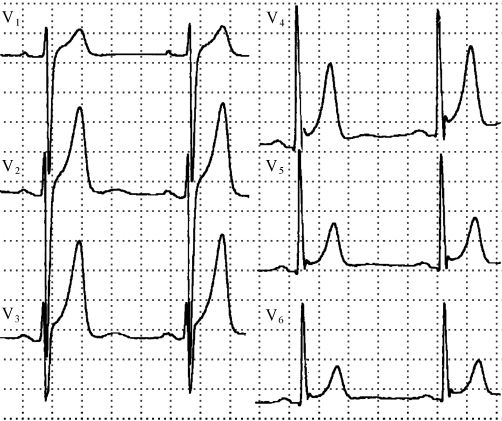
\includegraphics[width=3.38542in,height=2.84375in]{./images/Image00732.jpg}
 \captionsetup{justification=centering}
 \caption{急性肾功能衰竭、高钾血症患者(血钾6.2mmol/L)出现P波振幅降低、帐篷状T波}
 \label{fig45-4}
  \end{figure} 

(2)各种传导阻滞:当血K\textsuperscript{+}
>6.5mmol/L时,可出现窦房传导阻滞、心房内传导阻滞、房室传导阻滞、束支阻滞及不定型心室内传导阻滞等。

(3)P波振幅渐低、时间渐宽,直至消失,出现窦-室传导:当血K\textsuperscript{+}
>8.0mmol/L时,冲动在心房内的传导、除极均受到抑制,直至心房麻痹,但窦性冲动仍可通过结间束、房间束传至房室交接区直至心室,形成窦-室传导。

(5)QRS-T波群融合形成正弦波:当血K\textsuperscript{+}
>10mmol/L时,QRS波群振幅明显降低、时间更宽,T波振幅反趋降低而圆钝,两者融合形成正弦波;频率缓慢而不规则,Q-T间期延长,直至出现心脏停搏或心室扑动、颤动而死亡(图\ref{fig45-5})。

\begin{figure}[!htbp]
 \centering
 \includegraphics[width=5.1875in,height=1.36458in]{./images/Image00733.jpg}
 \captionsetup{justification=centering}
 \caption{糖尿病、酮症酸中毒、高钾血症患者(血钾8.6mmol/L)出现QRS-T波群融合形成正弦波、心室颤动(引自朱同新)}
 \label{fig45-5}
  \end{figure} 

(6)偶尔可使心房颤动暂时转为窦性节律及出现异常Q波、ST段抬高和J波酷似急性心肌梗死(图\ref{fig44-19})或Brugada波等。

4.血K\textsuperscript{+} 浓度异常与心电图改变的关系

血K\textsuperscript{+}
浓度高低并不一定与心电图改变平行一致。因心电图改变取决于心肌细胞内K\textsuperscript{+}
含量,血清钾测定并不能及时真实地反映心肌细胞内K\textsuperscript{+}
含量,如急性失钾时,血钾已降低,但心电图检查无异常改变;又如慢性失钾时,由于细胞内K\textsuperscript{+}
释放到细胞外,血钾测定可在正常范围内,但心电图检查已显示低钾血症改变。此外,Na\textsuperscript{+}
、Ca\textsuperscript{2+}
等电解质及酸碱平衡失调亦可改变钾对心肌的影响,如低钠血症、低钙血症、酸中毒可加重高钾血症异常的心电图改变。

5.鉴别诊断

高钾血症早期出现的T波高耸、Q-T间期缩短,需与早复极综合征、短Q-T间期综合征、超急性期心肌梗死、左心室舒张期负荷过重、脑血管意外、变异型心绞痛等引起T波高耸相鉴别。

\protect\hypertarget{text00053.htmlux5cux23subid639}{}{}

\section{血钙异常的心电图改变}

\protect\hypertarget{text00053.htmlux5cux23subid640}{}{}

\subsection{低钙血症}

当血清钙<1.75mmol/L时,便称为低钙血症。常见于慢性肾功能衰竭、甲状旁腺功能减退等。低钙血症主要引起动作电位平台期Ca\textsuperscript{2+}
内流减慢使2相时间延长。心电图表现为ST段呈水平型延长(>0.16s)、Q-T间期延长(图\ref{fig45-6})。需注意与心内膜下心肌缺血相鉴别。

\begin{figure}[!htbp]
 \centering
 \includegraphics[width=5.8125in,height=2.27083in]{./images/Image00734.jpg}
 \captionsetup{justification=centering}
 \caption{女性,65岁,慢性肾功能不全、低钙(1.4mmol/L)及低钾血症(2.4mmol/L)。显示2:1传导的二度房室传导阻滞、ST段呈水平型延长、U波增高、Q-T间期延长、符合低钙及低钾血症的心电图改变}
 \label{fig45-6}
  \end{figure} 

\protect\hypertarget{text00053.htmlux5cux23subid641}{}{}

\subsection{高钙血症}

当血清钙>3.0mmol/L时,便称为高钙血症。常见于甲状旁腺功能亢进、多发性骨髓瘤、骨转移癌等。高钙血症主要引起动作电位2相时间缩短。心电图表现为ST段缩短或消失,Q-T间期缩短及U波增高;严重高钙血症时,可出现各种传导阻滞、室性心律失常等。需与短Q-T间期综合征相鉴别。

\protect\hypertarget{text00053.htmlux5cux23subid642}{}{}

\section{血镁异常的心电图改变}

正常血清镁浓度为0.75~1.25mmol/L。约99\%的镁分布在细胞内,而细胞外液中的镁仅占1\%,其中约60\%为游离的Mg\textsuperscript{2+}
。游离的Mg\textsuperscript{2+}
在体内具有多种生理功能:酶的激活剂、调节神经肌肉及心血管的兴奋性、降低细胞膜的通透性及组成骨盐的成分等。

\protect\hypertarget{text00053.htmlux5cux23subid643}{}{}

\subsection{低镁血症}

1.基本概念

当血清镁浓度<0.75mmol/L时,便称为低镁血症。较常见,大医院约占10\%,在急救中心,其发生率可达65\%。常见于长期禁食、厌食、严重腹泻、急性胰腺炎、长期使用利尿剂、糖尿病酮症酸中毒及甲状腺功能亢进等疾病。

2.低镁血症对心肌细胞的影响

低镁血症时,心肌细胞膜上的Na\textsuperscript{+} -K\textsuperscript{+}
-ATP酶活性降低,引起细胞内K\textsuperscript{+}
外流减小,静息电位负值减小,兴奋性增高;因Mg\textsuperscript{2+}
有阻断浦肯野纤维等快反应细胞的Na\textsuperscript{+}
内流作用,低镁血症时,这种阻断作用减弱,以致Na\textsuperscript{+}
内流增快、增多,4相除极化加速,自律性增高。随着心肌细胞兴奋性和自律性的增高,易发生心律失常。低镁血症时,因血管平滑肌细胞内Ca\textsuperscript{2+}
含量增高,血管平滑肌对缩血管物质反应性增强,可引起冠状动脉痉挛,导致心肌缺血,甚至心肌梗死。低镁血症时,常合并低钾血症和低钙血症,故在低钾血症或低钙血症时,如经补钾、补钙后仍不能纠正,则应考虑有缺镁的存在,并且也只有同时补镁后方能见效。

3.心电图改变

(1)类似低钾血症时的ST-T改变,有时出现T波电交替现象(图\ref{fig45-7})。

\begin{figure}[!htbp]
 \centering
 \includegraphics[width=5.1875in,height=0.67708in]{./images/Image00735.jpg}
 \captionsetup{justification=centering}
 \caption{低镁血症(0.61mmol/L)患者出现T波电交替现象(引自郭继鸿)}
 \label{fig45-7}
  \end{figure} 

(2)可出现各种心律失常及传导阻滞。

\protect\hypertarget{text00053.htmlux5cux23subid644}{}{}

\subsection{高镁血症}

当血清镁浓度>1.25mmol/L时,便称为高镁血症。但血镁不超过2.0mmol/L时,对机体影响很小,只有当血镁高达3.0mmol/L时,才会出现症状。常见于肾功能衰竭、甲状腺功能减退、肾上腺皮质功能减退、镁摄入过多等。高镁血症时,心肌兴奋性降低,传导抑制。心电图改变类似高钾血症的改变,表现为心动过缓、完全性房室传导阻滞,QRS波群增宽,甚至心脏停搏。

\protect\hypertarget{text00054.html}{}{}

\protect\hypertarget{text00054.htmlux5cux23chapter54}{}{}

\chapter{药物影响及其诱发的心律失常}

\protect\hypertarget{text00054.htmlux5cux23subid645}{}{}

\section{洋地黄对心脏的作用及心电图改变}

\protect\hypertarget{text00054.htmlux5cux23subid646}{}{}

\subsection{洋地黄对心脏的作用}

(1)增强心肌收缩力、降低交感神经张力、间接兴奋迷走神经:洋地黄有抑制心肌细胞膜Na\textsuperscript{+}
-K\textsuperscript{+}
泵ATP酶系统作用,促使肌浆网释放Ca\textsuperscript{2+}
,增强心肌收缩力,改善心功能。

(2)降低窦房结自律性:与洋地黄降低窦房结4相去极化速度和间接兴奋迷走神经作用有关,可出现窦性心动过缓、窦性停搏。

(3)延长窦房交接区、房室交接区的有效不应期并降低其传导速度:可出现窦房传导阻滞、房室传导阻滞,降低心房扑动、颤动时的心室率。

(4)缩短房室旁道的有效不应期并加快其传导速度:预激综合征合并心房颤动、房室逆向型折返性心动过速时,严禁使用洋地黄类药物。

(5)缩短心房肌的有效不应期并加快其传导速度:与洋地黄直接对心房肌作用和间接兴奋迷走神经作用有关。低浓度时,间接兴奋迷走神经作用占优势,降低心房内异位灶的自律性;高浓度时,洋地黄直接作用占优势,心房内异位灶的自律性增高。

(6)增强心室内异位灶的自律性及折返性心律失常:洋地黄能使浦肯野纤维4相去极化加速、膜电位负值减小更接近阈电位,导致其自律性增高,出现室性心律失常。膜电位负值减小后,膜反应性和传导速度减慢,易形成折返性心律失常。

(7)缩短心室肌的2相动作电位,使Q-T间期缩短。

(8)增强触发活动而引发心律失常:洋地黄过量时,细胞膜上Na\textsuperscript{+}
-K\textsuperscript{+} 泵受到抑制,使细胞内Na\textsuperscript{+}
增加,通过Na\textsuperscript{+} -Ca\textsuperscript{2+}
交换,大量Ca\textsuperscript{2+} 内流,细胞内Ca\textsuperscript{2+}
超负荷,引起延迟后除极而诱发心律失常。

\protect\hypertarget{text00054.htmlux5cux23subid647}{}{}

\subsection{洋地黄治疗量时心电图表现}

(1)鱼钩样ST-T改变:以R波为主导联ST段呈下斜型压低、T波负正双相或倒置,其前肢与ST段融合,呈鱼钩样改变。

(2)Q-T间期缩短。

(3)U波增高。

\protect\hypertarget{text00054.htmlux5cux23subid648}{}{}

\subsection{洋地黄中毒时的心电图特征}

洋地黄中毒时,主要是由兴奋性增高引起的各种心律失常及由抑制作用引起的缓慢性心律失常和传导阻滞,或两者联合作用引起的心律失常。最能预示洋地黄中毒的心电图表现有频发多形性或多源性室性早搏二联律、室性心动过速、双向性心动过速、高度或三度房室传导阻滞、非阵发性房室交接性或室性心动过速、心房扑动或颤动等。

(1)室性心律失常:①频发单源性、多源性或多形性室性早搏,多呈二、三联律,是洋地黄中毒最常见、最早出现的心律失常,尤其是在心房颤动基础上出现(图\ref{fig13-19});②室性心动过速,可呈短阵性或持续性,常为洋地黄中毒的晚期表现(图\ref{fig46-1}),死亡率高达68\%~100\%;③非阵发性室性心动过速或加速的室性逸搏心律;④双向性室性心动过速,为重度中毒表现,常在心房颤动基础上发生(图\ref{fig46-2}),死亡率很高;⑤心室颤动。

\begin{figure}[!htbp]
 \centering
 \includegraphics[width=5.71875in,height=2.15625in]{./images/Image00736.jpg}
 \captionsetup{justification=centering}
 \caption{冠心病、心房颤动患者。Ⅱ导联系服用洋地黄后连续记录,显示心房颤动、频发加速的室性逸搏(77次/min)、加速的房室交接性逸搏或室性融合波(上行R\textsubscript{13})、频发短阵性室性心动过速伴心室折返径路内不典型4:3文氏现象、完全性干扰性房室分离,提示洋地黄中毒}
 \label{fig46-1}
  \end{figure} 


\begin{figure}[!htbp]
 \centering
 \includegraphics[width=5.6875in,height=1.26042in]{./images/Image00737.jpg}
 \captionsetup{justification=centering}
 \caption{心房颤动服用洋地黄患者。aVF、V\textsubscript{1}导联同步记录,显示双向性室性心动过速,提示洋地黄中毒}
 \label{fig46-2}
  \end{figure} 


(2)房室交接性心律失常:①非阵发性房室交接性心动过速或加速的房室交接性逸搏心律;②过缓的房室交接性逸搏及其逸搏心律。

(3)房性心律失常:①阵发性房性心动过速伴房室传导阻滞;②心房扑动或颤动。

(4)房室分离或房室传导阻滞:①原有心房颤动,经洋地黄治疗后,出现加速的房室交接性逸搏心律合并房室分离,诊断洋地黄中毒具有很高的特异性,且发生率较高(图\ref{fig13-20}、图\ref{fig13-21});②出现二度、高度、三度房室传导阻滞合并房室交接性或室性逸搏及其逸搏心律(图\ref{fig13-17}、图\ref{fig13-18});③出现一度、二度Ⅰ型房室传导阻滞,前者为洋地黄中毒早期表现,后者为最常见表现之一,其阻滞部位多发生在房室结内,很少发生在房室结以下。

(5)双重性心动过速:出现非阵发性或阵发性房性心动过速、非阵发性或阵发性房室交接性心动过速、非阵发性或阵发性室性心动过速或上述6种心律失常的不同组合。

(6)窦性心律失常:出现显著的窦性心动过缓、窦性停搏或窦房传导阻滞。

(7)原有心房颤动,经洋地黄治疗后心室率反而更快者,多数是洋地黄中毒的表现。

\protect\hypertarget{text00054.htmlux5cux23subid649}{}{}

\subsection{非洋地黄中毒性心律失常}

有些心律失常尽管在洋地黄化或使用洋地黄病人中出现,但它们与洋地黄中毒并无关系,有学者称为“非洋地黄中毒性心律失常”,其心电图表现有以下6点:①并行心律型室性早搏、室性心动过速;②阵发性房室交接性心动过速;③由房室结以下部位阻滞引起的二度Ⅱ型房室传导阻滞;④由房室结以下部位阻滞引起的三度房室传导阻滞伴加速的室性逸搏心律或室性逸搏心律;⑤各种的心室内传导阻滞,如束支阻滞、分支阻滞及不定型心室内传导阻滞;⑥窦性心动过速。

\protect\hypertarget{text00054.htmlux5cux23subid650}{}{}

\subsection{识别洋地黄中毒心电图特征的临床意义}

洋地黄类药物是治疗充血性心力衰竭、快速型心房颤动的常用药物之一,其治疗量约为中毒剂量的60\%,故临床上约有20\%的患者发生中毒现象,表现为心律失常或(和)房室传导阻滞。在中毒病例中约3\%~21\%因心脏毒性反应而死亡。因此,早期识别并及时处理洋地黄中毒引起的心律失常,具有极为重要的临床意义。

\protect\hypertarget{text00054.htmlux5cux23subid651}{}{}

\subsection{诊断洋地黄中毒应注意的问题}

(1)洋地黄中毒和用量大小无绝对比例关系,小剂量洋地黄中毒,多与肾功能减退、心肌严重受损、电解质紊乱或应用利尿剂等因素有关。

(2)洋地黄中毒可毫无自觉症状,须观察对比用药前后症状及心电图改变,如心率、传导情况等。

(3)在洋地黄治疗过程中,临床上遇及以下4种特征性改变,应疑及中毒,及时做心电图检查:①正常心率或快速心率转为心动过缓;②正常心率时突然出现心动过速;③不规则的心律变为规则的心律;④呈现有规律的不规则心律。

(4)洋地黄中毒的有些表现可能不为人们所注意,如窦性心动过速及(或)心力衰竭恶化,易误认为洋地黄用量不足而进一步加大剂量,加重中毒程度。凡是在洋地黄加量后心率反而加快及(或)心力衰竭恶化者,应考虑中毒可能。

(5)原有心力衰竭在使用洋地黄后曾一度好转而又突然或进行性加重,并发展为难治性心力衰竭者,应警惕洋地黄中毒。

(6)快速型心房颤动伴心力衰竭时经洋地黄治疗后,心室率仍较快且伴有室性早搏出现,该早搏出现不一定是洋地黄中毒的表现,可能是洋地黄用量不足、心力衰竭尚未纠正所致,可采用“西地兰耐量试验”观察判断。

(7)正确对待血清地高辛浓度的测定,需密切结合临床加以评估与判断。

\protect\hypertarget{text00054.htmlux5cux23subid652}{}{}

\section{抗心律失常药物的致心律失常作用}

\protect\hypertarget{text00054.htmlux5cux23subid653}{}{}

\subsection{抗心律失常药物的分类}

根据药物对心肌细胞的电生理作用不同而分为4类。

(1)Ⅰ类药物:又称为膜稳定剂,抑制Na\textsuperscript{+}
内流及起搏细胞4相除极化速度,增加K\textsuperscript{+}
外流作用。可分为:①Ⅰa类药物,如奎尼丁、普鲁卡因酰胺等;②Ⅰb类药物,如利多卡因、美律西平(慢心律)等;③Ⅰc类药物,如普罗帕酮(心律平)、乙吗噻嗪等。

(2)Ⅱ类药物:为β受体阻滞剂,如倍他乐克等。阻断β肾上腺素能受体和限制Ca\textsuperscript{2+}
内流作用,降低窦房结和异位起搏点的自律性;也有轻度抑制Na\textsuperscript{+}
内流及K\textsuperscript{+} 外流作用,缩短不应期,减慢传导速度。

(3)Ⅲ类药物:为复极抑制剂,如胺碘酮、索他洛尔等,主要抑制2、3相的K\textsuperscript{+}
外流,使动作电位时间和有效不应期延长。

(4)Ⅳ类药物:为Ca\textsuperscript{2+}
拮抗剂,如维拉帕米(异搏定)、硫氮酮等。阻止慢反应细胞Ca\textsuperscript{2+}
内流,降低窦房结、房室结细胞的自律性,延长房室结的不应期及传导时间。

\protect\hypertarget{text00054.htmlux5cux23subid654}{}{}

\subsection{致心律失常作用的概念、机制及诊断标准}

1.基本概念

由抗心律失常药物引起新的心律失常或使原有的心律失常加重现象,称为致心律失常作用。绝大多数抗心律失常药物均有致心律失常作用,尤其是有心肌损害时。胺碘酮致心律失常作用最小。由抗心律失常药物引起的传导异常,则不属于致心律失常作用的范畴。

2.致心律失常作用的机制

(1)机体的特异质反应。

(2)药物本身的毒性作用。

(3)与心肌复极、不应期不一致有关:正常和异常心肌组织的传导性、不应期及复极过程等电生理特性均有明显差异,局部心肌血流差异还可影响药物在组织中的分布和结合,从而影响电生理参数;若合并电解质紊乱、酸碱平衡失调,则可增强心脏对药物的敏感性;延长Q-T间期药物,在心动过缓或长短间歇后,易诱发尖端扭转型室性心动过速。

3.致心律失常作用的诊断标准

(1)抗心律失常药物治疗过程中,出现新的快速性室性心律失常而无其他诱因。

(2)室性早搏加重:对照期为1~50次/h者,次数增加10倍;对照期为51~100次/h者,增加5倍;对照期为101~300次/h者,增加4倍;对照期为≥301次/h者,则增加3倍。

(3)室性心动过速发作时频率显著增快者。

(4)室性心律失常发生变异:由短阵性室性心动过速发展为持续性室性心动过速、由单一室性心动过速发展为扭转性、多形性、多源性室性心动过速或心室颤动。

(5)终止快速型室性心律失常的难度增大。

\protect\hypertarget{text00054.htmlux5cux23subid655}{}{}

\subsection{常用抗心律失常药物的心电图改变及致心律失常作用的特征}

(一)胺碘酮(可达龙)

1.作用机制及适应证

为Ⅲ类药物,主要作用于动作电位2、3相,抑制K\textsuperscript{+}
外流,使动作电位和有效不应期延长,尚有抑制Ca\textsuperscript{2+}
内流及Na\textsuperscript{+}
内流,并兼有抗心绞痛、β受体阻滞剂作用。适用于各种早搏、心动过速、阵发性心房颤动及扑动。

2.心电图表现

(1)减慢心率:可使基础心率降低10\%~15\%,当心率较快时,减慢心率作用更为明显。

(2)T波时间增宽,呈双峰切迹、振幅降低。

(3)Q-T间期延长:以T波时间延长为主,若延长超过正常最高值25\%,应减量或停药。

(4)可出现U波振幅增高。

(5)剂量过大时,可引起扭转型室性心动过速、心室颤动、窦性停搏及高度房室传导阻滞等。

(二)普罗帕酮(心律平)

1.作用机制及适应证

为Ⅰc类药物,抑制动作电位0相的快Na\textsuperscript{+}
通道开放、延长有效不应期及阻断β受体的效能。对异位刺激或折返机制所致的心律失常有显著的效果。

2.心电图表现

(1)减慢心率引起窦性心动过缓。

(2)可出现P-R间期延长及QRS波群时间增宽。

(3)可出现Q-T间期延长。

(4)剂量过大或毒性作用时,可出现窦性停搏、高度窦房或房室传导阻滞、多形性或尖端扭转型室性心动过速及心室颤动等。

(三)美律西平(慢心律)

1.作用机制及适应证

为Ⅰb类药物,除抑制Na\textsuperscript{+}
内流外,突出的作用是加速复极期K\textsuperscript{+}
外流,缩短不应期。改善心室内传导,尚能抑制浦肯野纤维4相除极化,降低心室内异位起搏点的自律性。适用于室性心律失常的治疗。

2.心电图表现

(1)对窦房结功能正常者无明显影响,对其功能不全者,可引起窦性心动过缓、窦性停搏等。

(2)剂量过大或静脉注射时,可出现房室传导阻滞、心室颤动、心室停搏等。

(四)利多卡因

为Ⅰb类药物,作用机制与美西律相似,对室性心律失常是安全有效的。常于给药的开始两天内出现窦性心动过缓、窦性停搏、窦房传导阻滞、房室传导阻滞或心室内传导阻滞等。

(五)苯妥英钠

为Ⅰb类药物,作用机制与美律西平相似,仅用于洋地黄中毒引起的室性心律失常。剂量过大或给药过快时,可出现窦性心动过缓、房室传导阻滞或心脏骤停等。

(六)倍他乐克(美托洛尔)

为β受体阻滞剂,兼有弱的细胞膜抑制作用,用于窦性心动过速、早搏及心绞痛、高血压的治疗。可引起窦性心动过缓、窦房或房室传导阻滞等。

(七)维拉帕米(异搏定)

为Ca\textsuperscript{2+}
拮抗剂,能抑制心脏及房室传导,减慢心率。对阵发性室上性心动过速、分支型室性心动过速及短偶联间期尖端扭转型室性心动过速综合征有效。当剂量过大或静脉注射过快时,可出现窦性心动过缓、窦性停搏、房室传导阻滞或室性心律失常,甚至出现心脏、呼吸骤停等;能加速或改变房室旁道为顺向性传导,增加心室率,可使预激综合征合并室上性心动过速、心房颤动者发生心室颤动而死亡。

(八)阿托品

为胆碱能M受体拮抗剂,对窦房结具有双重作用。小剂量(<0.4mg)引起迷走神经张力增高,降低窦性频率,诱发房室交接性逸搏及逸搏心律;大剂量(>0.5mg)可解除迷走神经对心脏的抑制作用,使窦性频率加快,可诱发窦性心动过速、多源性室性早搏、室性心动过速等。

(九)肾上腺素(副肾素)

为肾上腺素能受体兴奋剂,直接兴奋α、β受体,使周围血管收缩,心率加快,血压升高。用于支气管哮喘、过敏性休克及心脏骤停复苏者。剂量过大或静脉注射过快,可引起室性心律失常,如室性早搏、室性心动过速甚至心室颤动。

\protect\hypertarget{text00054.htmlux5cux23subid656}{}{}

\subsection{如何预防及减少药物致心律失常作用}

(1)使用抗心律失常药物时,应对患者作出全面、正确的评估,去除诱因,治疗病因,注意药物个体化及关注药物致心律失常作用,是减少致心律失常作用的关键。

(2)严格掌握药物的应用指征。

(3)尽量先用一种药物,并从小剂量开始,治疗前、后应予24h动态心电图监测。

(4)多种抗心律失常药物联合治疗仅适用于单一药物最大耐受量治疗无效或致命性心律失常的患者需要额外保护时,需注意协同和拮抗作用。

(5)使用抗心律失常药物前、后应测定并及时纠正电解质紊乱、酸碱平衡失调。

(6)注意抗心律失常药物和其他药物相互不良作用及配伍禁忌。

(7)静脉给药时,应进行心电监护。

(8)长期服药者,最好能做血液药物浓度监测。

\protect\hypertarget{text00055.html}{}{}

\protect\hypertarget{text00055.htmlux5cux23chapter55}{}{}

